%%%%%%%%%%%%%%%%%%%%%%%%%%%%%%%%%%%%%%%%%%%%%%%%%%%%%%%%%%%%%
%LUNGHEZZA STIMATA 3-4 FACCIATE DI TESTO PER GIORNATA DI LAB%
%%%%%%%%%%%%%%%%%%%%%%%%%%%%%%%%%%%%%%%%%%%%%%%%%%%%%%%%%%%%%
%%%%IN TOTALE CIRCA 15 FACCIATE DI TESTO IMMAGINI ESCLUSE%%%%
%%%%%%%%%%%%%%%%%%%%%%%%%%%%%%%%%%%%%%%%%%%%%%%%%%%%%%%%%%%%%
%Di solito nei papers accademici / tecnici si usa sempre
%la forma impersonale, quindi "E' stata misurata la corrente..."
%oppure "si è proceduto a misurare la corrente...."
%anziché "Abbiamo misurato la corrente..."

\documentclass[journal]{IEEEtran}

\usepackage[italian]{babel}

% *** CITATION PACKAGES ***
\usepackage[style=ieee]{biblatex} 
\bibliography{analog.bib}    %your file created using JabRef
\usepackage{hyperref}
% *** MATH PACKAGES ***
\usepackage{amsmath}
 \usepackage{multirow}

% *** PDF, URL AND HYPERLINK PACKAGES ***
\usepackage{url}
\usepackage{makeidx}
% correct bad hyphenation here
\hyphenation{op-tical net-works semi-conduc-tor}
\usepackage{graphicx}  %needed to include png, eps figures
\usepackage{float}  % used to fix location of images i.e.\begin{figure}[H]
\makeindex

\begin{document}

% paper title
\title{Laboratorio di elettronica analogica\\ 
%\small{1 gennaio 2020}
}

% author names 
\author{\begin{center}Matteo Barbagiovanni\textsuperscript{1},
        Stefano Barbero\textsuperscript{2},
        Federico Malnati\textsuperscript{3},
        Valerio Pagliarino\textsuperscript{4},
        {\small \\
        \textsuperscript{1}
        matteo.barbagiovanni@edu.unito.it -
        \textsuperscript{2}
        stefano.barbero376@edu.unito.it
        \textsuperscript{3}
        federico.malnati@edu.unito.it -
        \textsuperscript{4}
        valerio.pagliarino@edu.unito.it}
        \end{center}}% <-this % stops a space
        
% The report headers
\markboth{Università degli Studi di Torino - C.d.L. Triennale in Fisica - 21/10/21 - A.A. 2021-2022    \quad   \quad \quad \quad   \quad \quad \quad  \quad   \quad \quad \quad   \quad \quad LABORATORIO DI ELETTRONICA \quad \quad }%do not delete next lines
{Shell \MakeLowercase{\textit{et al.}}: Bare Demo of IEEEtran.cls for IEEE Journals}

% make the title area
\maketitle

% As a general rule, do not put math, special symbols or citations
% in the abstract or keywords.
\begin{abstract}  
Oggi la ricerca in fisica in ogni ambito è supportata in modo fondamentale dall'elettronica e dall'informatica che permettono l'acquisizione dei dati, la loro analisi e l'esecuzione di simulazioni; l'elettronica digitale ha rivoluzionato le tecniche di calcolo, ma l'elettronica analogica continua ad essere cruciale, poiché interviene nel processo di trasduzione dell'osservabile fisica in un segnale elettrico e nel condizionamento di quest'ultimo fino alla conversione in digitale ad opera di \textit{ADCs}, \textit{TDCs} o altri sistemi. Non stupisce allora il fatto che in molti sistemi di misura e rivelazione l'elettronica analogica rappresenti il vero limite alle prestazioni dell'apparato. In questa relazione di laboratorio verranno analizzati alcuni circuiti analogici di rilievo per la strumentazione fisica: dopo una breve introduzione agli strumenti e lo studio qualitativo di un raddrizzatore a singola semionda realizzato con diodo al silicio, si prenderanno in esame alcune applicazioni degli amplificatori operazionali. Dapprima si verificherà il funzionamento in configurazione ad anello aperto come discriminatore di soglia e verrà misurato lo \textit{slew rate}, dopodiché si passerà ad alcune configurazioni retroazionate che consentono l'amplificazione dei segnali con guadagno prefissato e il calcolo di operazioni matematiche tra segnali analogici come integrali, derivate, somme e differenze. Successivamente verrà realizzato mediante due amplificatori operazionali un comparatore con isteresi (trigger di Schmitt) in grado di discriminare un segnale a cui è stato sommato del rumore mediante il secondo stadio analogico. Si concluderà questa relazione con l'analisi di un semplice circuito di read-out per un fotomoltiplicatore al silicio (SiPM) che consentirà di calcolare il guadagno del sensore e con alcune verifiche delle leggi di propagazione dei segnali su linee coassiali.
%Concluso, da rileggere
\end{abstract}

%%%%%%%%%%%%%%%%%%%%%%%%%%%%%%%%%%%%%%%%%%
\section{\textbf{Strumentazione utilizzata}} %Valerio

\IEEEPARstart{I}{} circuiti qui descritti sono stati implementati mediante l'uso di componentistica \textit{COTS} \textit{(off the shelf)} in standard \textit{through hole}, più maneggevole rispetto a quella \textit{SMD}, installata su breadboard. Le interconnessioni sono state realizzate con normali jumper mentre le alimentazioni sono state collegate utilizzando connettori a banana. I segnali sono stati misurati con l'oscilloscopio utilizzando sonde passive attenuate X10.
Segue oltre una brevissima dei principali strumenti di misura e generatori utilizzati.

\subsection{\textbf{Oscilloscopio Tektronix TBS1104}}

\begin{figure}[h!]
  \centering
  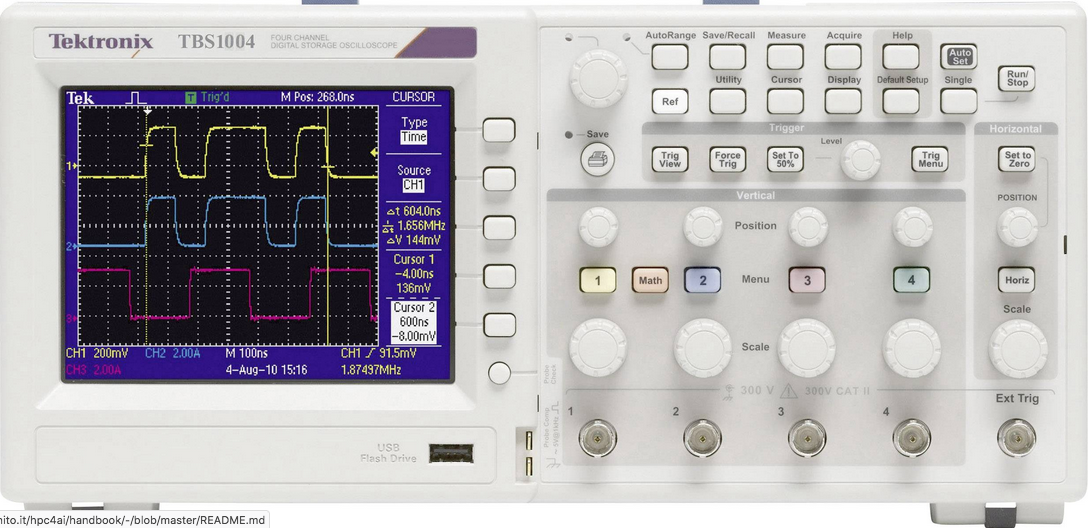
\includegraphics[width=0.18\textwidth]{lab-reports/Schematics-and-graphics/TEK Osc.png}
\end{figure}

La maggior parte delle misure di tensione e tempo è stata realizzata con un \textit{digital storage oscilloscope (DSO)} Tektronix 1104 con banda passante di 70 MHz, frequenza di campionamento massima di 1 GSa/s che consente fino a 5 ns/div di risoluzione temporale, 4 canali e 2.5K punti di memoria per finestra di acquisizione, risoluzione verticale di 8 bit e sensibilità fino a 10 mV/div. \cite{A}

\subsection{\textbf{Oscilloscopio Rhode \& Schwartz RTB2004}}

\begin{figure}[h!]
  \centering
  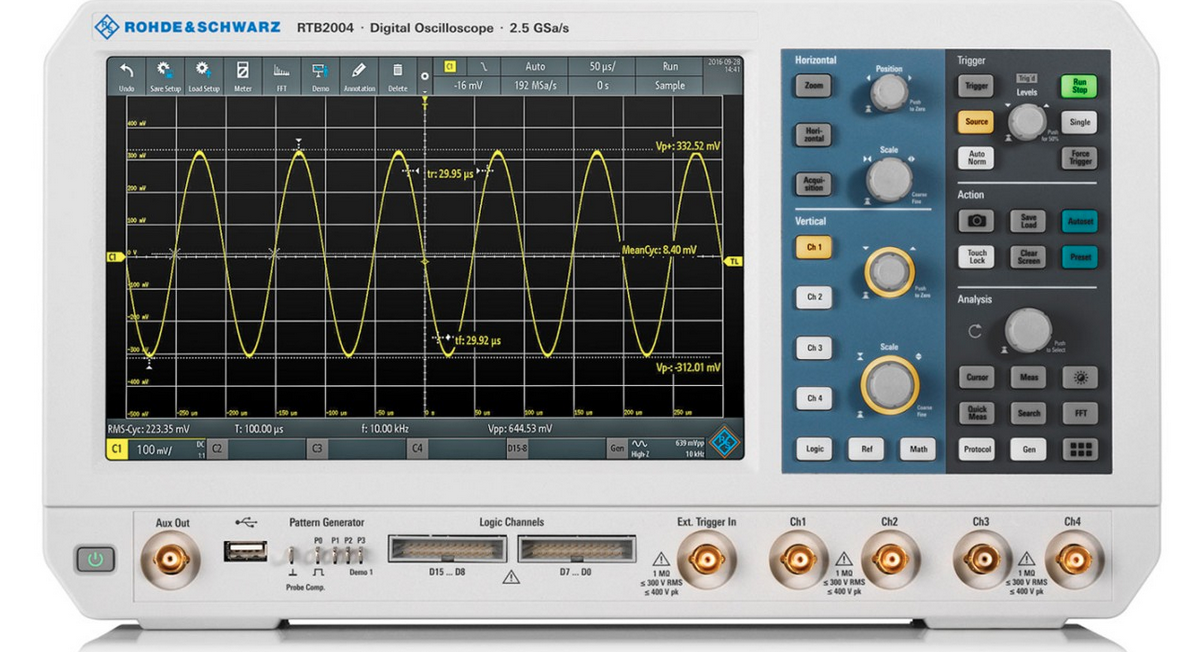
\includegraphics[width=0.18\textwidth]{lab-reports/Schematics-and-graphics/RS Osc.png}
\end{figure}

Per visualizzare il segnale in uscita dal fotomoltiplicatore al silicio è stata invece utilizzato un oscilloscopio di fascia più alta, quale il Rhode \& Schwarz RTB2004 dotato di un ADC a 10 bit con banda passante di 70 MHz e frequenza di campionamento massima di 2.5 GSa/s che consente raggiungere una risoluzione temporale di 1 ns/div. Quest'ultima caratteristica, unita alla sensibilità fino a 1 mV/div, ha permesso di visualizzare correttamente i segnali molto deboli e veloci prodotti dal sensore quando viene eccitata una singola cella. \cite{B}

\subsection{\textbf{Generatori di funzioni Rigol DG1022Z e Siglent SDG1010}}

\begin{figure}[h!]
  \centering
  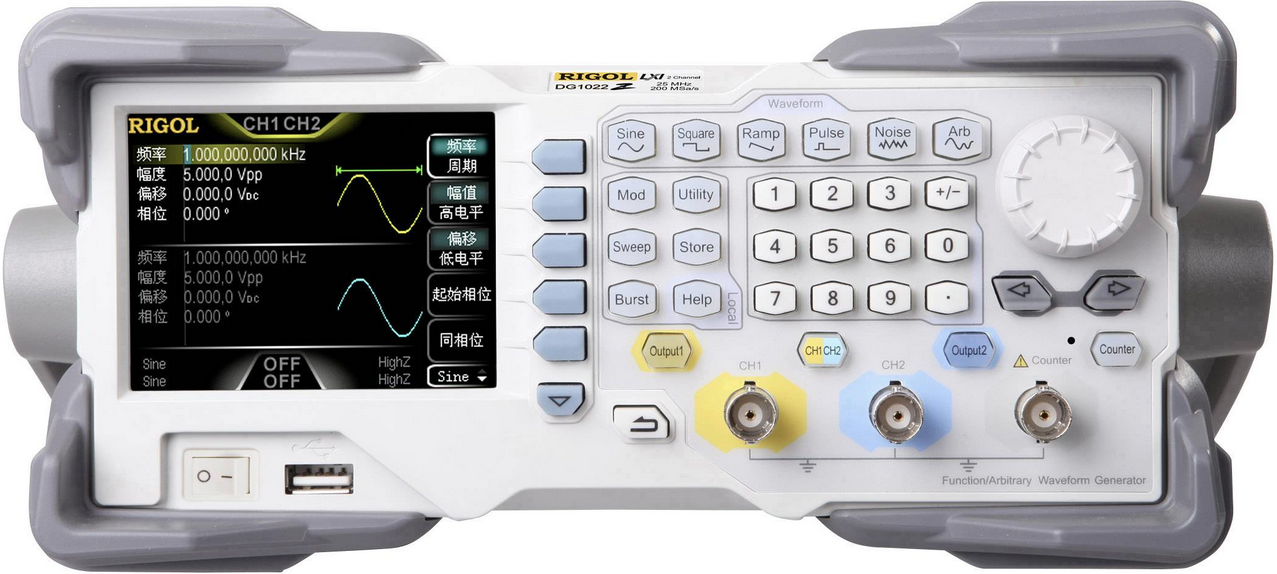
\includegraphics[width=0.18\textwidth]{lab-reports/Schematics-and-graphics/RIGOL Gen.png}
\end{figure}

\begin{figure}[h!]
  \centering
  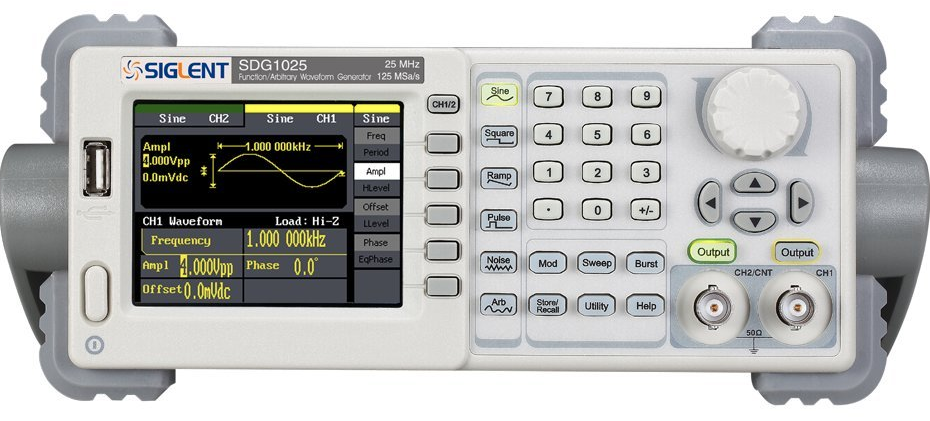
\includegraphics[width=0.18\textwidth]{lab-reports/Schematics-and-graphics/SIGLENT Gen.png}
\end{figure}

Questi due generatori di segnali arbitrari basati sulla sintesi digitale diretta (DDS) sono stati impiegati per il pilotaggio dei circuiti. Il secondo dispositivo è stato impiegato per la generazione dell'impulso di tensione per l'alimentazione del led nell'esperienza di caratterizzazione del SiPM, mentre il primo apparecchio per tutte le altre misure. Il generatore \textit{Rigol} ha una banda passante massima di 25 MHz, una frequenza di campionamento del DAC di 100 MSa/s e una risoluzione verticale di 14 bit. Il generatore \textit{Siglent}, invece, ha una banda passante di 10 MHz, una frequenza di campionamento del DAC di 125 MSa/s, una risoluzione verticale anch'esso di 14 bit e supporta la generazione di impulsi mediante la velocità "burst" con un fronte di salita / discesa minimo di 7 ns e una durata minima di 16 ns. Il generatore dispone di un'uscita di sincronismo in standard TTL con durata degli impulsi $> 50$ ns che abbiamo utilizzato per pilotare il trigger esterno dell'oscilloscopio Rhode \& Schwarz. \cite{E} \cite{G}

\subsection{\textbf{Generatore di impulsi veloci Keithley 3390}}

\begin{figure}[h!]
  \centering
  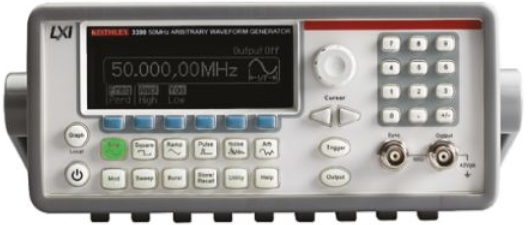
\includegraphics[width=0.18\textwidth]{lab-reports/Schematics-and-graphics/KEIT Gen.png}
\end{figure}


Per lo studio della propagazione di segnali attraverso una linea di trasmissione coassiale è stato fondamentale disporre di un generatore di segnali in grado di produrre impulsi sufficientemente veloci, in relazione al tempo di propagazione lungo la linea, con fronti più ripidi possibile. Per questo motivo è stato impiegato un generatore di segnali arbitrari Keithley 3390, anch'esso basato sulla tecnologia della sintesi digitale diretta, che dispone di una banda passante analogica di 50 MHz, una durata minima degli impulsi di 20 ns e un fronte di salita minimo di 10 ns. \cite{F}

\subsection{\textbf{Multimetro digitale Meterman 35XP e alimentatore da banco duale GW-Instek GPS-4303}}
Il corredo di strumentazione è stato completato con multimetro digitale Meterman 35XP utilizzato per misurare tensioni, resistenze e capacità, soprattutto in fase montaggio e verifica dei circuiti e da un generatore di tensione GW-Instek GPS-4303 con 4 canali a tensione e corrente variabile utilizzabili per fornire alimentazione duale all'amplificatore operazionale impiegato. La tensione proveniente da questo alimentatore è risultato in alcuni casi un po' rumorosa, pertanto sono stati aggiunti sulla breadboard dei condensatori livellanti in parallelo con valori nominali di $\sim$ 22 nF e $\sim$ 100 nF. Il multimetro ha una risoluzione di 3+3/4 cifre, un'accuratezza nelle misure di tensione DC di 0.5 \% della lettura + 1 * ultima cifra fino a 1KV e un'accuratezza nelle misure di resistenza di 1.0 \% della lettura + 4 * ultima cifra fino a 40 M$\Omega$. Per l'accuratezza nelle misure di capacità si rimanda al datasheet. L'alimentatore è invece in grado di fornire sui canali utilizzati fino a 30V / 5A. \cite{C} \cite{D}.
%%%%%%%%%%%%%%%%%%%%%%%%%%%%%%%%%%%%%%%%%%
\section{\textbf{Ponte raddrizzatore a diodi a singola semionda}} %Matteo
\subsection{\textbf{Introduzione all'esperienza}}
In molteplici applicazioni si ha la necessità di convertire tensioni alternate in tensioni continue (AC/DC). Uno dei modi più immediati per ottenere tale risultato è quello di sfruttare raddrizzatori non controllati, quali raddrizzatori a singola/doppia semi-onda, a ponte monofase/trifase o esafase realizzati utilizzando diodi al silicio, che consentono di gestire alte potenze in spazio ridotto con elevata affidabilità. Il diodo al silicio è un componente attivo non lineare la cui forma funzionale della corrente in rispetto alla tensione è descritta dalla \textit{relazione di Shockley}: 
\begin{equation}
    I_{D} = I_{0}(e^{V/\eta V_T}-1)
\end{equation}

 dove $I_{0}$ rappresenta la corrente di saturazione inversa, il termine $V_{T}$ è la tensione termica e $\eta$ è il fattore di idealità, dipendente dalle caratteristiche costruttive e dai materiali con cui è realizzato il diodo.
\subsection{\textbf{Componentistica e circuito}}

\begin{figure}[H]%[!ht]
\begin{center}
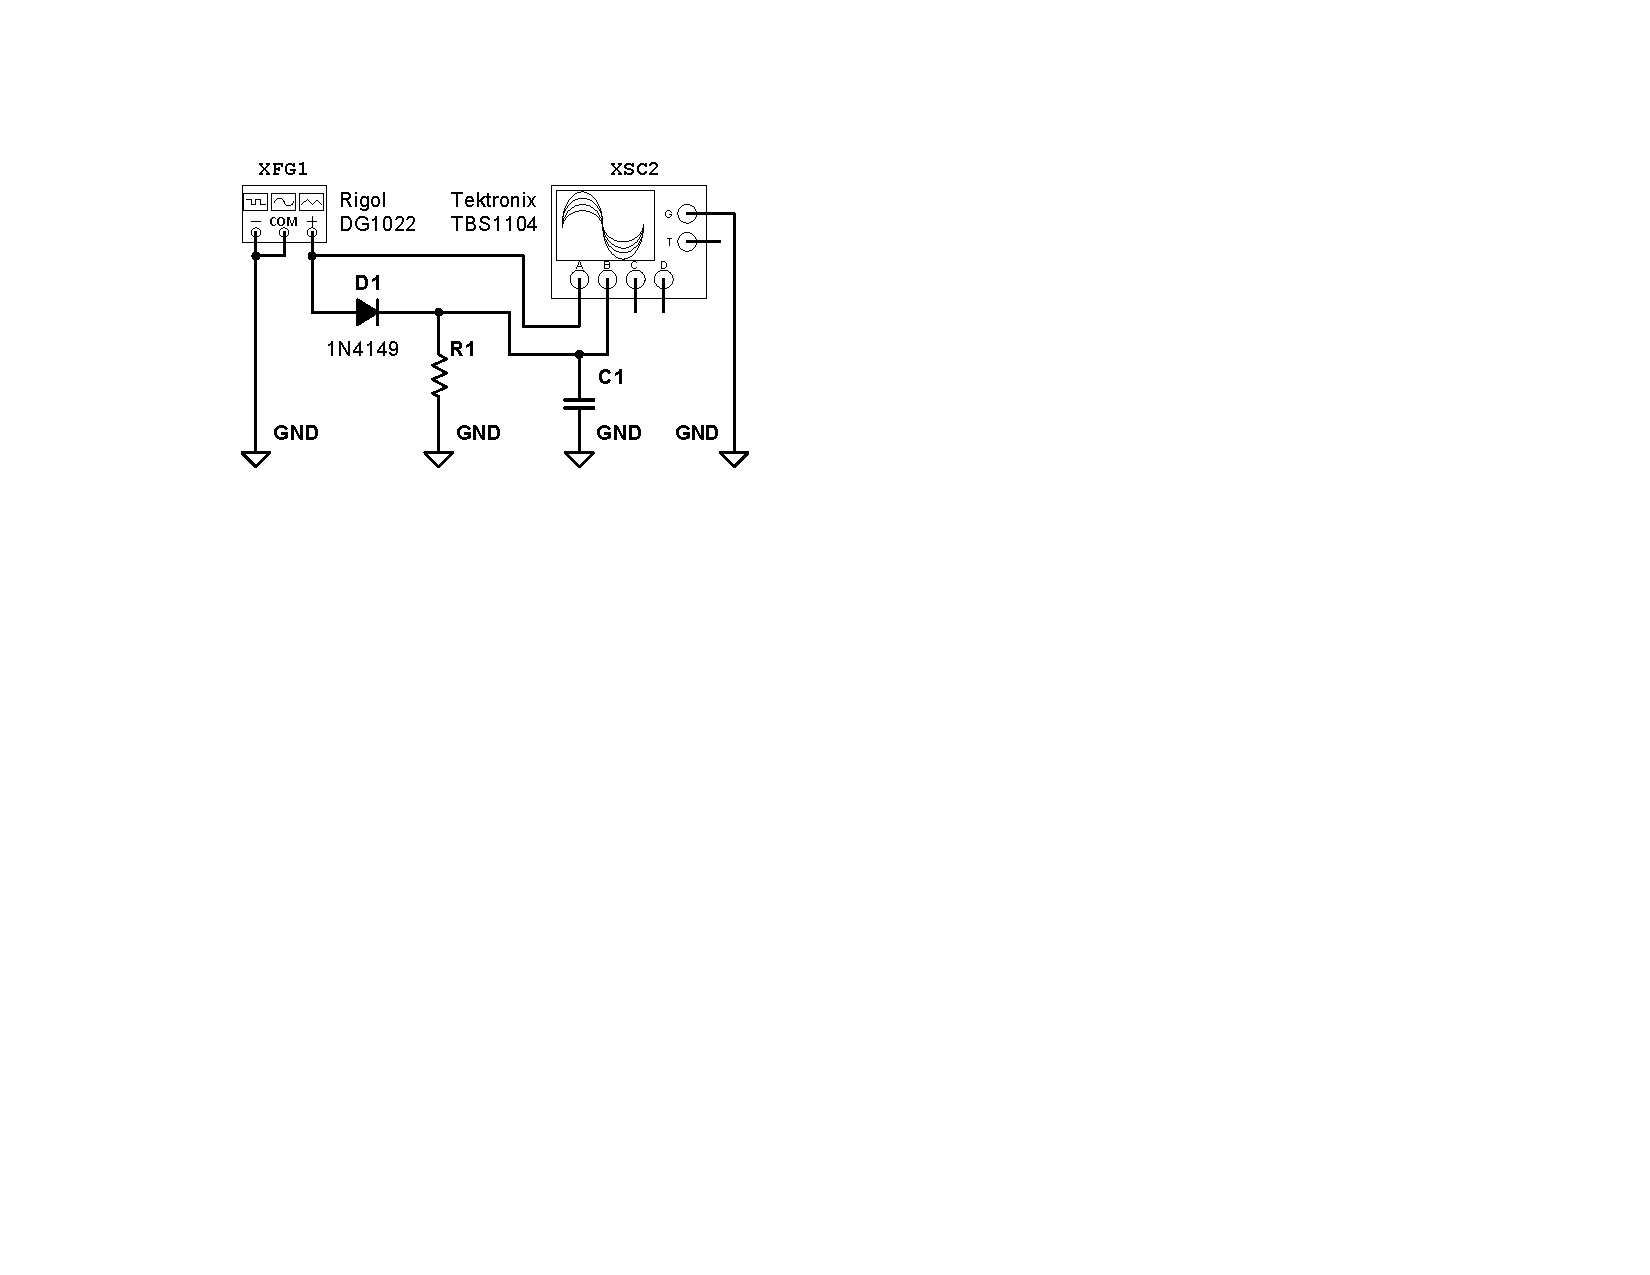
\includegraphics[width=0.32\textwidth]{sch-simulations/output/Diode-rectifier.pdf}
\caption{Schema del circuito elettrico per la caratterizzazione del diodo al Silicio.}
\label{fig:diode-rectifier}
\end{center}
\end{figure}

\vspace{-5mm}

La trattazione successiva riguarda i raddrizzatori a singola semionda ed in particolare l'implementazione del circuito in \textit{Fig. \ref{fig:diode-rectifier}}, realizzato tramite un unico diodo a cui può essere aggiunto un condensatore di filtraggio. In tale configurazione il condensatore si comporta come un filtro passa basso trasformando una tensione in ingresso impulsiva, in una di tipo continuo. 
Uno degli obiettivi nella realizzazione di un raddrizzatore è quello di minimizzare la \textit{tensione di ripple} rimanente, ciò è possibile regolando il valore della costante di tempo $\tau$ costituito dal carico e dal condensatore.
Analizzando il funzionamento del circuito in assenza del condensatore di livellamento, invece, si avrà in uscita un segnale impulsivo costituito solamente dalla semionda positiva oppure negativa, a seconda del verso in cui viene installato il diodo.

\subsection{\textbf{Caratterizzazione}}
In laboratorio è stato implementato il circuito della \textit{Fig. \ref{fig:diode-rectifier}} in assenza del condensatore di filtraggio in modo da poter osservare il comportamento del diodo.

\vspace{-5mm}

\begin{figure}[H]%[!ht]
\begin {center}
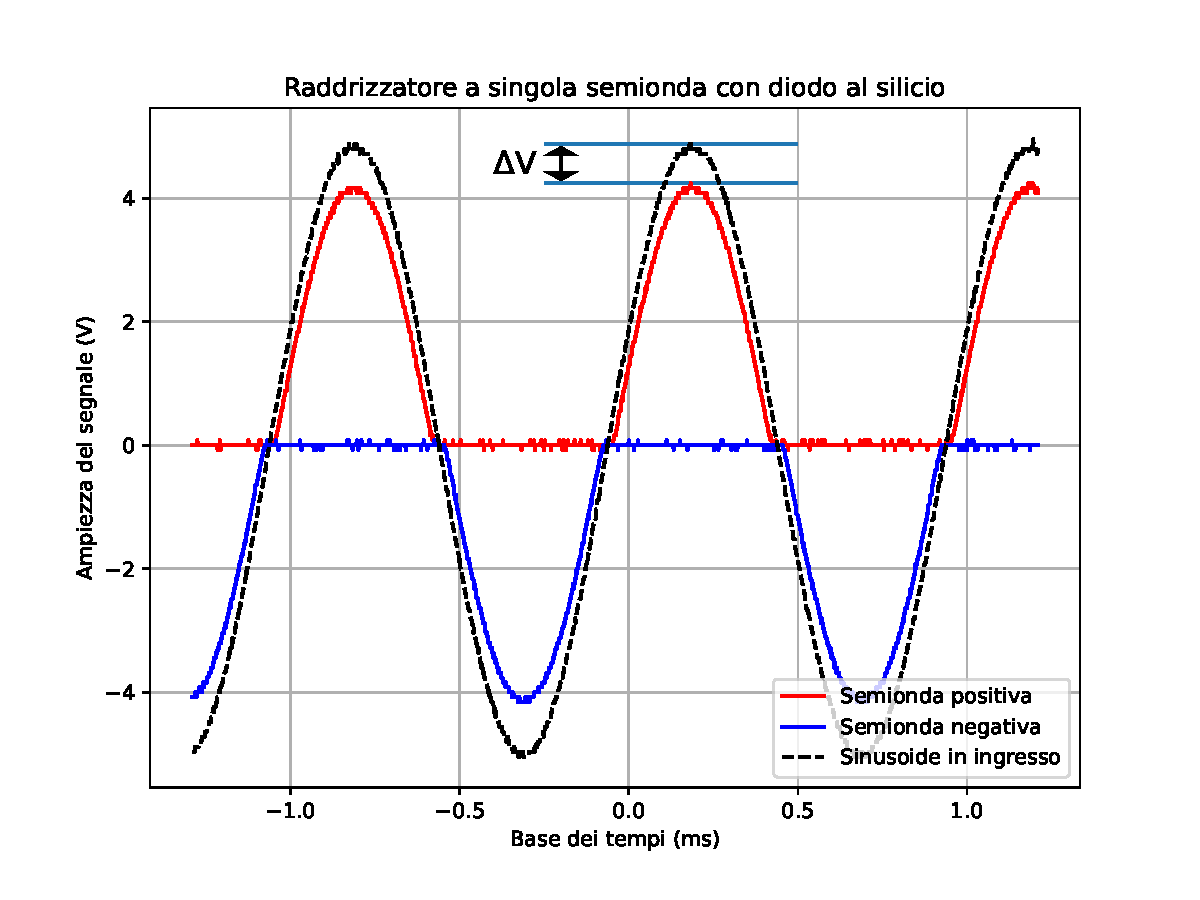
\includegraphics[width=0.50\textwidth]{analysis/output/half-wave-rectifier.pdf}
\caption{Grafico del segnale processato da un raddrizzatore a singola semionda con diodo al silicio}
\label{fig:half-wave}
\end {center}
\end{figure}


Si nota nel grafico \ref{fig:half-wave} una differenza di tensione di picco tra l'ingresso e l'uscita pari a $\Delta V = (0.64 \pm 0.05) V$ che è certamente compatibile con il valore atteso per la caduta di tensione ai capi del diodo, come confermato dal risultato del \textit{Test di Gauss}, che riporta una variabile statistica $Z = 0.56$, minore di $Z_{critico}$ = 1.96.
\subsection{\textbf{Discussione dei risultati}}
In conclusione l'analisi qualitativa del comportamento del diodo presenta una totale consistenza con la teoria.


%%%%%%%%%%%%%%%%%%%%%%%%%%%%%%%%%%%%%%%%%%
\section{\textbf{Introduzione all'amplificatore operazionale}}
Passiamo ora allo studio di una serie di circuiti notevoli che fanno uso di amplificatori operazionali (OPA), con l'obiettivo di amplificare, integrare, derivare o eseguire altre operazioni notevoli su segnali analogici. Questi componenti sono altamente versatili e sono utilizzati in quasi tutti gli ambiti in cui è necessario il condizionamento di un segnale analogico. Sono modellizzabili come amplificatori differenziali con impedenza in ingresso teoricamente infinita, impedenza di uscita teoricamente nulla, banda passante infinita e guadagno a circuito aperto teoricamente infinito. Nella realizzazione pratica è possibile raggiungere per queste grandezze valori molto grandi o molto piccoli grazie all'utilizzo di processi di fabbricazione integrati che consentono di realizzare su un singolo \textit{die} circuiti analogici complessi multistadio (almeno stadio di ingresso differenziale, stadio di guadagno, stadio di uscita). Nelle esperienze che seguiranno verranno utilizzati OPA \textbf{LM741} prodotti dalla \textit{Texas Instruments} con package DIP, dispositivi a basso costo alimentati in tensione duale $\pm$ 15 V con \textit{slew rate} tipico di 0.5 V/$\mu$s, larghezza di banda di 1.5 MHz e guadagno tipico per grandi segnali a T = 298 K di 50 V/mV. \cite{H}

%%%%%%%%%%%%%%%%%%%%%%%%%%%%%%%%%%%%%%%%%%
\section{\textbf{Configurazione ad anello aperto invertente (zero-crossing detector)}} %Stefano
\subsection{\textbf{Introduzione all'esperienza}}


\begin{figure}[h]%[!ht]
\begin {center}
\includegraphics[width=0.38\textwidth]{sch-simulations/output/opa-open-loop-inverting.pdf}
\caption{Configurazione ad anello aperto invertente. Si nota l'assenza di controreazione}
\label{fig:circ_open_loop_inv}
\end {center}
\end{figure}

La prima analisi effettuata con l'amplificatore operazionale è stata in configurazione invertente ad anello aperto. Lo scopo era di verificare che fin da piccoli valori di segnale in ingresso, non inserendo alcun feedback, l'amplificazione ad anello aperto fosse sufficiente a raggiungere la zona di saturazione dell'OPA, ottenendo in uscita un valore prossimo alla tensione di alimentazione fornita.
Questo comportamento dell'operazionale rende possibile il suo utilizzo come discriminatore o nel caso di un ingresso collegato a massa come  \textit{zero-crossing detector}.

\subsection{\textbf{Caratterizzazione}}
Di seguito si descrive il calcolo del valore di segnale in ingresso a partire dal quale si raggiunge la saturazione.

\begin{figure}[h]%[!ht]
\begin {center}
\includegraphics[width=0.48\textwidth]{analysis/output/opa-open-loop-inv-zero-crossing.pdf}
\caption{Nell'immagine si apprezzano l'intensità dell'amplificazione e l'inversione del segnale}
\label{fig:open_loop_inv_zc_1}
\end {center}
\end{figure}

Come segnale in ingresso si è scelto di generare un'onda sinusoidale di ampiezza $500$ $mV$ e frequenza di $1$ $kHz$, attendendosi una serie di saturazioni a segno alterno dell'uscita dell'amplificatore ($ \approx 15 V$ per sinusoide negativa, $\approx -15 V$ per sinusoide positiva).

\begin{figure}[h]%[!ht]
\begin {center}
\includegraphics[width=0.48\textwidth]{analysis/output/opa-open-loop-inv-zero-crossing-z2.pdf}
\caption{In rosso sono segnati i livelli di saturazione, in nero i punti di zero-crossing. La scala del segnale di ingresso è stata ingrandita ed è riportata sulla sinistra}
\label{fig:open_loop_inv_zc_2}
\end {center}
\end{figure}

Il segnale in uscita è compreso tra $-14.0 \pm 0.5 V $  e $14.6 \pm 0.5 V$.
Si sceglie dunque di considerare in saturazione l'amplificatore per valori superiori a $14.1 V$ o inferiori a $-13.5 V$. Il segnale è infatti soggetto a inevitabili oscillazioni, e si è dunque valutato l'intervallo di fluttuazione dei segnali a questi livelli riscontrando questi valori come estremi.

Di seguito i valori per cui vengono superate le soglie nei vari intervalli temporali: nella prima colonna è riportato l'intervallo in cui avviene la commutazione, nella seconda colonna il valore di tensione di saturazione che viene raggiunto, mentre nella terza colonna il valore assunto dal segnale in ingresso quando viene raggiunta la saturazione.

\newline
\vspace{4mm}

\begin{tabular}{|c|c|c|}
\hline
    t $\pm$ 0.05 {[}ms{]} & $V_{sat}$ $\pm 0.5$ {[}V{]} & $V_{in}$ $\pm 0.02$ {[}V{]} \\ \hline
-0.90 \textless t \textless -0.40 & -13.5 & 0.024  \\ \hline
-0.40 \textless t \textless 0.10  & 14.1  & -0.048 \\ \hline
0.10 \textless t \textless 0.60   & -13.5 & 0.032  \\ \hline
0.60 \textless t \textless 1.10   & 14.1  & -0.048 \\  \hline
\end{tabular}\\
\newline

Effettuando una media tra i due valori per la soglia alta si ottiene: $V_{zc} = -0.05 \pm 0.02 V$ .
Ripetendo il processo per la soglia bassa si ricava: $V_{zc} = 0.03 \pm 0.02 V$

I valori ottenuti sono in linea con le aspettative. Il loro ordine di grandezza è lo stesso dell'errore a loro associato e pertanto sono compatibili con un valore di tensione nullo.

\subsection{\textbf{Considerazioni finali}}
La configurazione usata si è dimostrata conforme alle aspettative, producendo un output costituito da saturazioni alterne in corrispondenza del passaggio per valori compatibili con zero. 

%%%%%%%%%%%%%%%%%%%%%%%%%%%%%%%%%%%%%%%%%%
\section{\textbf{Configurazione ad anello aperto non invertente}} %Stefano
\subsection{\textbf{Introduzione}}

Rispetto alla precedente configurazione il segnale di input è inserito nell'ingresso non invertente dell'amplificatore operazionale.
Ci si attende dunque un comportamento analogo al precedente, ma con amplificazione positiva. In questi casi il guadagno dipende dai parametri ibridi dell'OPA.

\subsection{\textbf{Caratterizzazione e considerazioni}}



Nella \textit{figura \ref{fig:open_loop_non_inv_zc}} si apprezza la concordanza di segno tra segnale in ingresso ed il segnale in uscita, come già detto nell'introduzione. E' inoltre apprezzabile il fatto che il livello di amplificazione rimanga costante nelle due configurazioni, come evidenziato dal cursore rosso.
Si conclude dicendo che in entrambi i casi la velocità con cui l'operazionale si porta in saturazione è limitata, producendo un segnale in uscita con dei fronti di salita e discesa non perfettamente verticali e non per motivazioni legate alla banda passante, ma bensì per la velocità di commutazione dell'OPA espressa dalla caratteristica dello \textit{slew rate} verrà analizzata quantitativamente nei paragrafi successivi. 

\begin{figure}[H]%[!ht]
\begin {center}
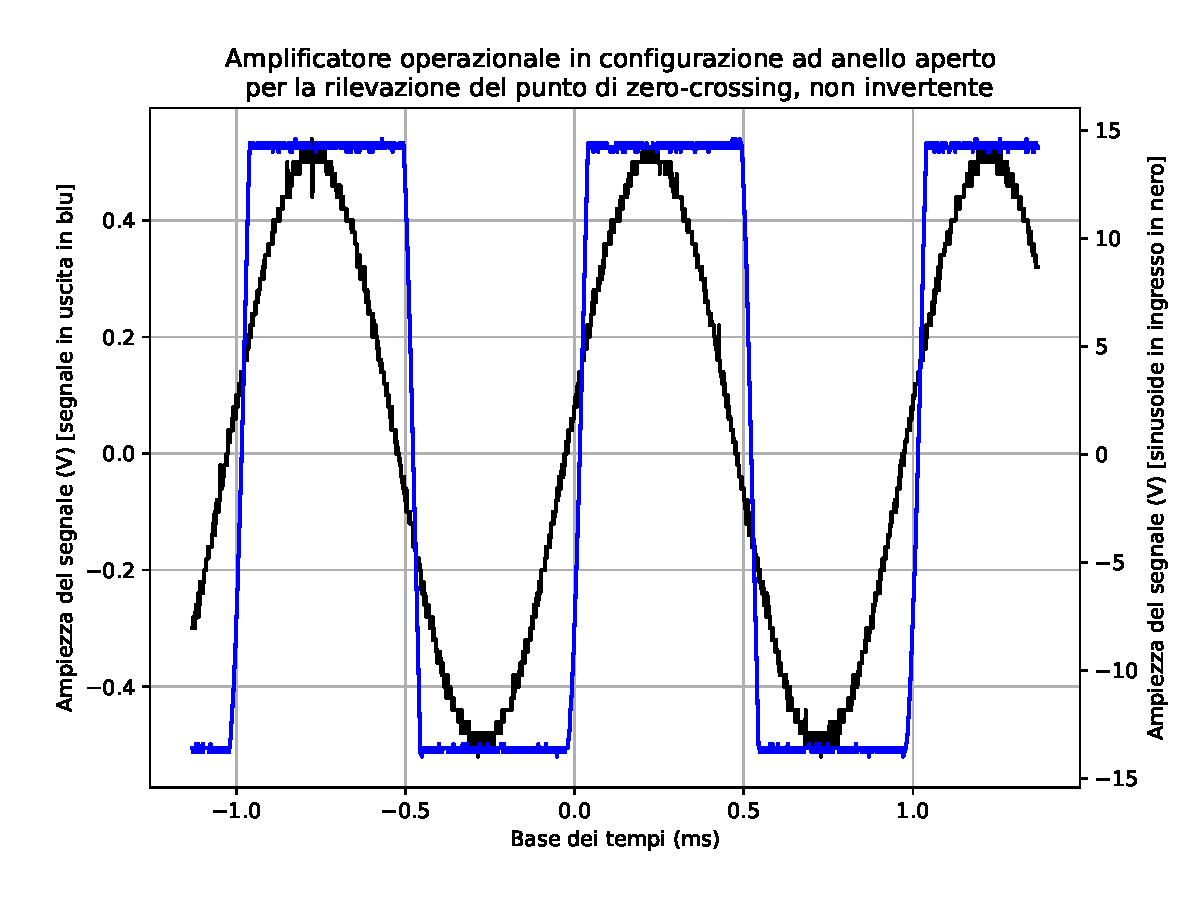
\includegraphics[width=0.52\textwidth]{analysis/output/OPA-open-loop-non-inv-zero-crossing-z2.pdf}
\caption{Nell'immagine si apprezza il segnale processato dal circuito ad anello aperto non invertente in blu. In rosso è riportata la soglia di commutazione che era stata calcolata per la configurazione invertente (compatibile con zero), in nero è visualizzato il segnale in ingresso.}
\label{fig:open_loop_non_inv_zc}
\end {center}
\end{figure}
%%%%%%%%%%%%%%%%%%%%%%%%%%%%%%%%%%%%%%%%%%

\section{\textbf{Configurazione ad anello aperto con soglia arbitraria}} %Stefano

\subsection{\textbf{Introduzione all'esperienza}}
\begin{figure}[H]%[!ht]
\begin {center}
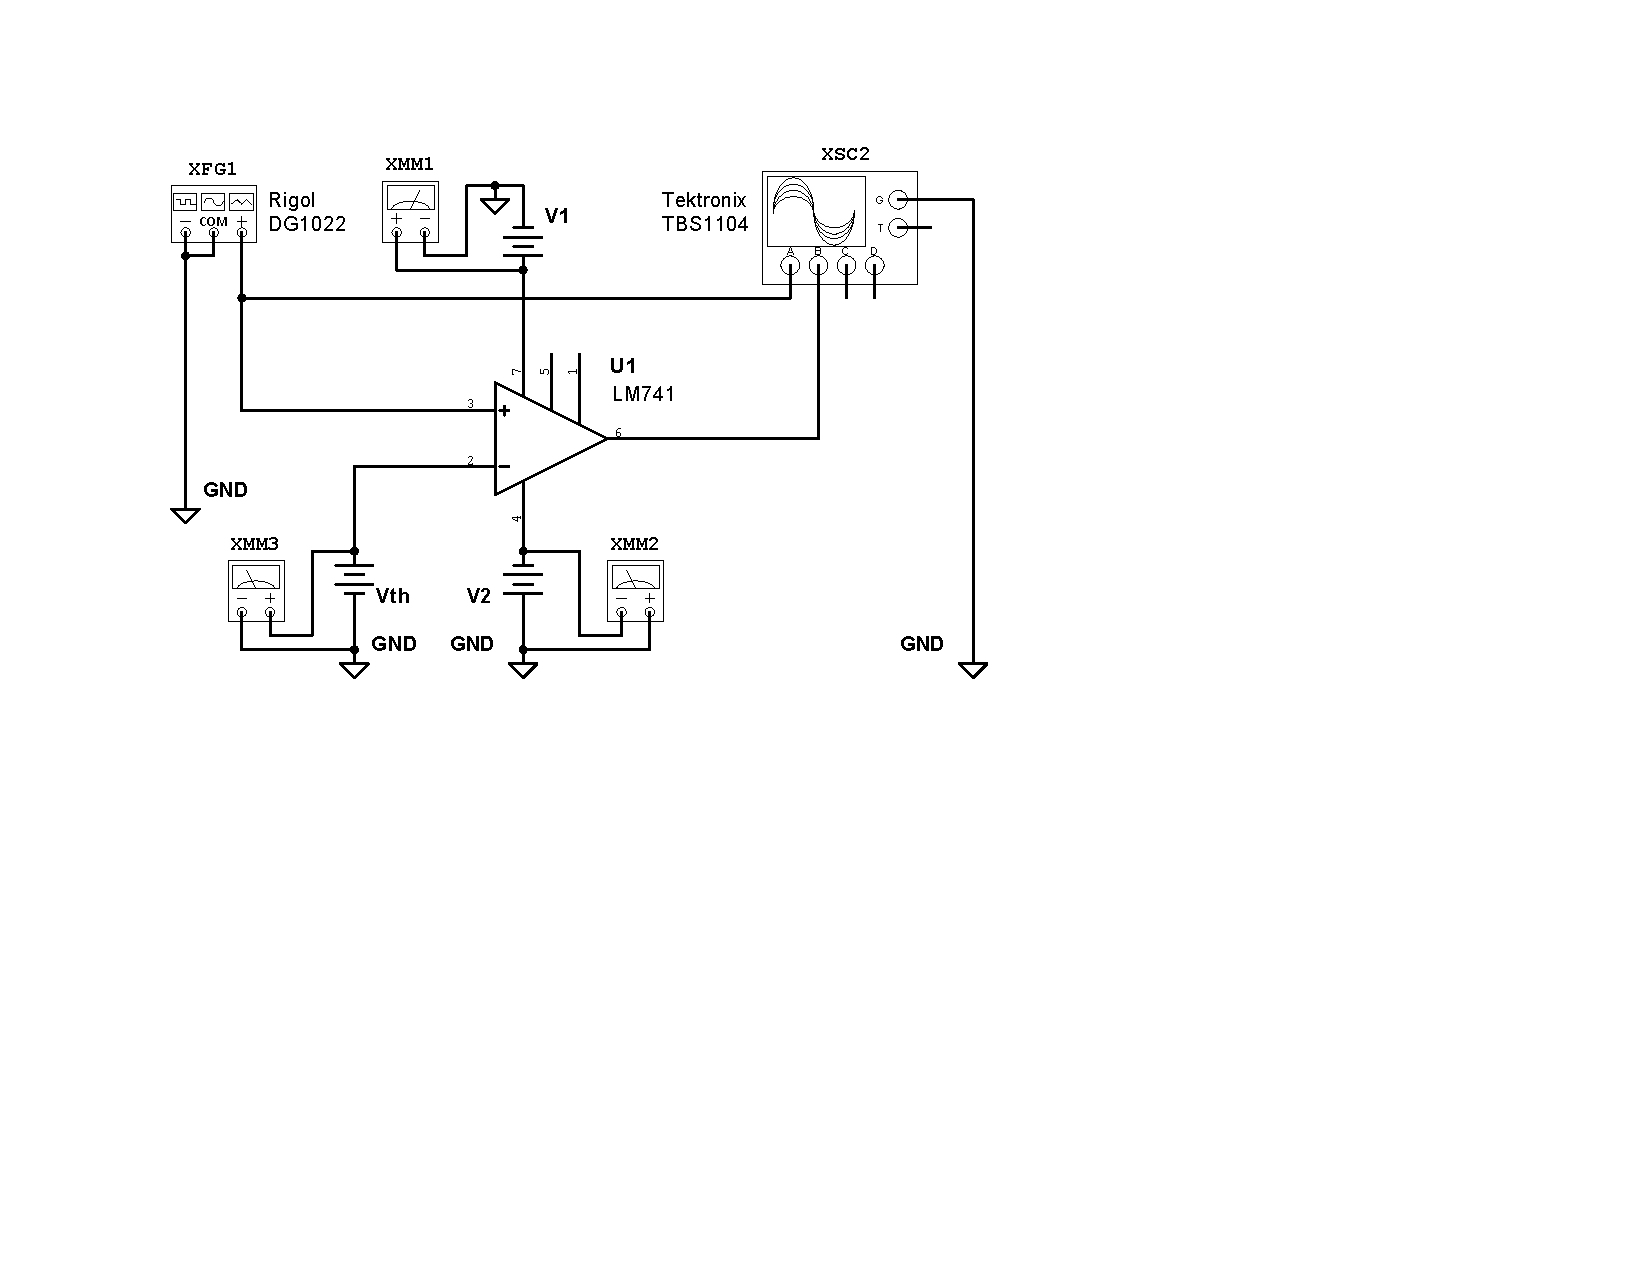
\includegraphics[width=0.38\textwidth]{sch-simulations/output/OPA-biased.pdf}
\caption{Amplificatore ad anello aperto: discriminatore con soglia a $V_{th} = 2.1 V$}
\label{fig:circ_open_loop_biased}
\end {center}
\end{figure}

La configurazione ad anello aperto dell'amplificatore può essere utile anche per discriminare segnali in ingresso rispetto ad una soglia arbitraria, diversa da $0V$, portando ad un apposito potenziale di riferimento l'ingresso dell'OPA non utilizzato per il segnale. Infatti lo stadio differenziale commuterà tra le regioni di saturazione quando la differenza tra i due ingressi passa per lo zero.
Non trattandosi di un circuito retroazionato, l'amplificazione sarà pari all'amplificazione di anello aperto, portando in saturazione l'uscita anche per piccole \textit{differenze} di segnale come verificato precedentemente.

\subsection{\textbf{Caratterizzazione}}
Nel caso in esame la soglia è stata posta a $V_{th} = 2.1$ $V$ utilizzando un canale a tensione variabile dell'alimentare collegato all'ingresso invertente, mentre in quello non invertente veniva fornito un segnale sinusoidale di ampiezza attesa $V_{pp} = 5.00$ $V$.

\begin{figure}[H]%[!ht]
\begin {center}
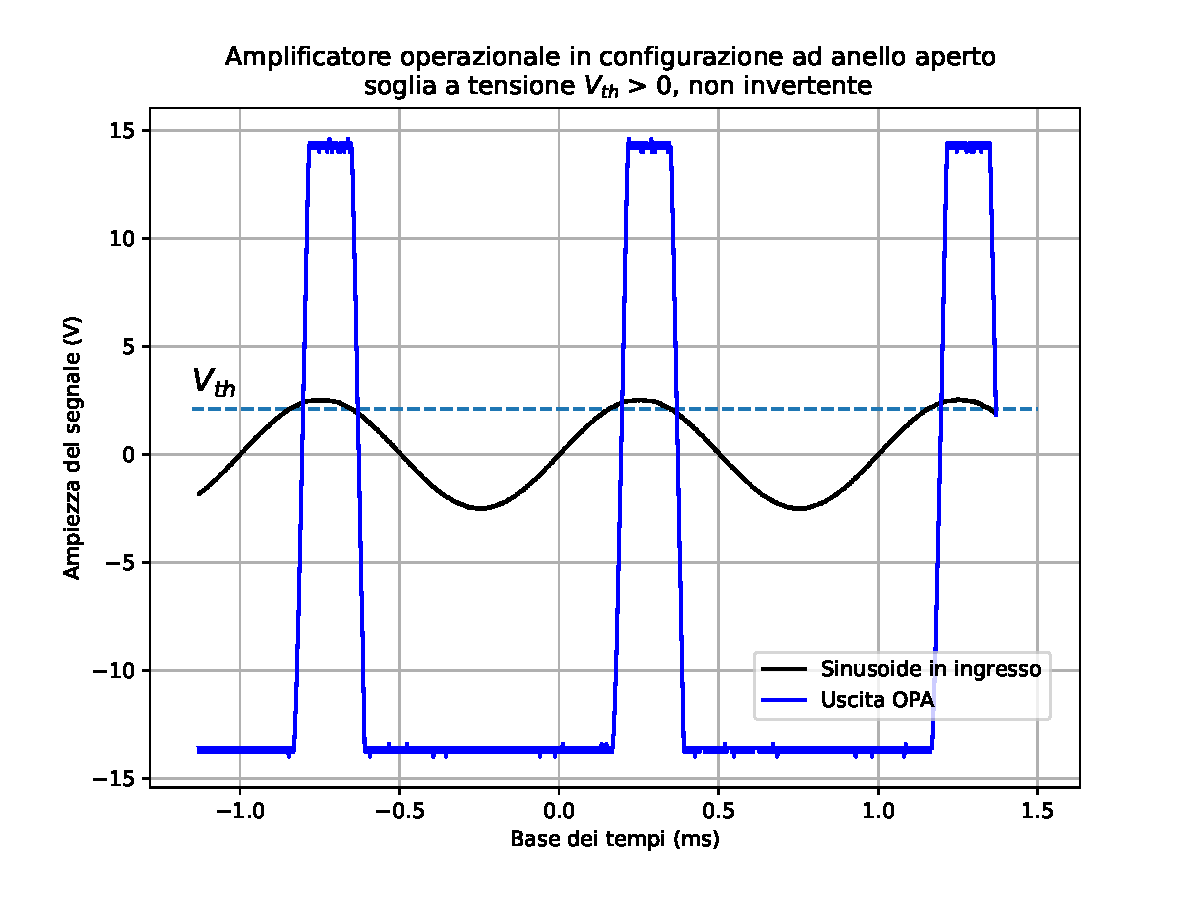
\includegraphics[width=0.52\textwidth]{analysis/output/OPA-open-loop-biased_threshold.pdf}
\vspace{-4mm}
\caption{Amplificatore ad anello aperto: discriminatore con soglia a $V = 2.1 V$}
\label{fig:biased_cross}
\end {center}


Dal confronto tra la figura \ref{fig:biased_cross} e la figura \ref{fig:open_loop_non_inv_zc} si può notare come in questo caso la soglia si trovi al valore atteso, comportando delle regioni di saturazione positiva e negativa non simmetriche. Di seguito è riportata la durata degli intervalli di commutazione nella prima colonna, mentre nelle successive la tensione di saturazione raggiunta e il ritardo rispetto all'effettivo punto di transito del segnale in ingresso per 2.1 V.
\end{figure}

\begin{tabular}{|c|c|c|c|}

\hline
$t  \pm 0.05 \ (ms)$ & $\Delta t \pm 0.07 \ (ms)$ & $V_{sat}$ $\pm 0.5 \ (V)$  \\ \hline
-0.80 \textless t \textless -0.60 & 0.20 & 14.1 \\ \hline %& 126 \\ \hline%
-0.60 \textless t \textless 0. 20 & 0.80 & -13.5 \\ \hline %& 763 \\ \hline%
0.20 \textless t \textless 0.40   & 0.20 & 14.1\\ \hline   %& 130 \\ \hline%
0.40 \textless t \textless 1.20   & 0.80 & -13.5 \\ \hline %& 766 \\ \hline
\end{tabular}

\subsection{\textbf{Discussione e conclusioni}}
In tutte e tre le configurazioni l'amplificatore ad anello aperto presenta il medesimo comportamento di base, nel primo caso in maniera invertente mentre in quelli successivi non invertente. Il circuito rispetta quindi le aspettative dimostrando però i limiti di velocità dovuti ad uno slew rate ridotto, caratteristica che verrà discussa in seguito.


%%%%%%%%%%%%%%%%%%%%%%%%%%%%%%%%%%%%%%%%%%
\section{\textbf{Amplificatore retroazionato non invertente}} %Matteo
\subsection{\textbf{Introduzione all'esperienza}}

La configurazione ad anello aperto finora trattata non offre la possibilità di utilizzare l'amplificatore operazionale in modo ottimale al di là dell'uso come discriminatore. Al fine di ottenere un'amplificazione regolabile e dipende esclusivamente da componenti esterni, anziché da parametri ibridi, nonché migliorare il controllo del dispositivo, si utilizza una rete di feedback negativo.
Il caso in esame utilizza una rete costituita da una resistenza $R_f$ che riporta parte della corrente in uscita nuovamente nell'ingresso invertente dell'amplificatore, dove è fornito il segnale in ingresso.

\begin{figure}[H]%[!ht]
\begin {center}
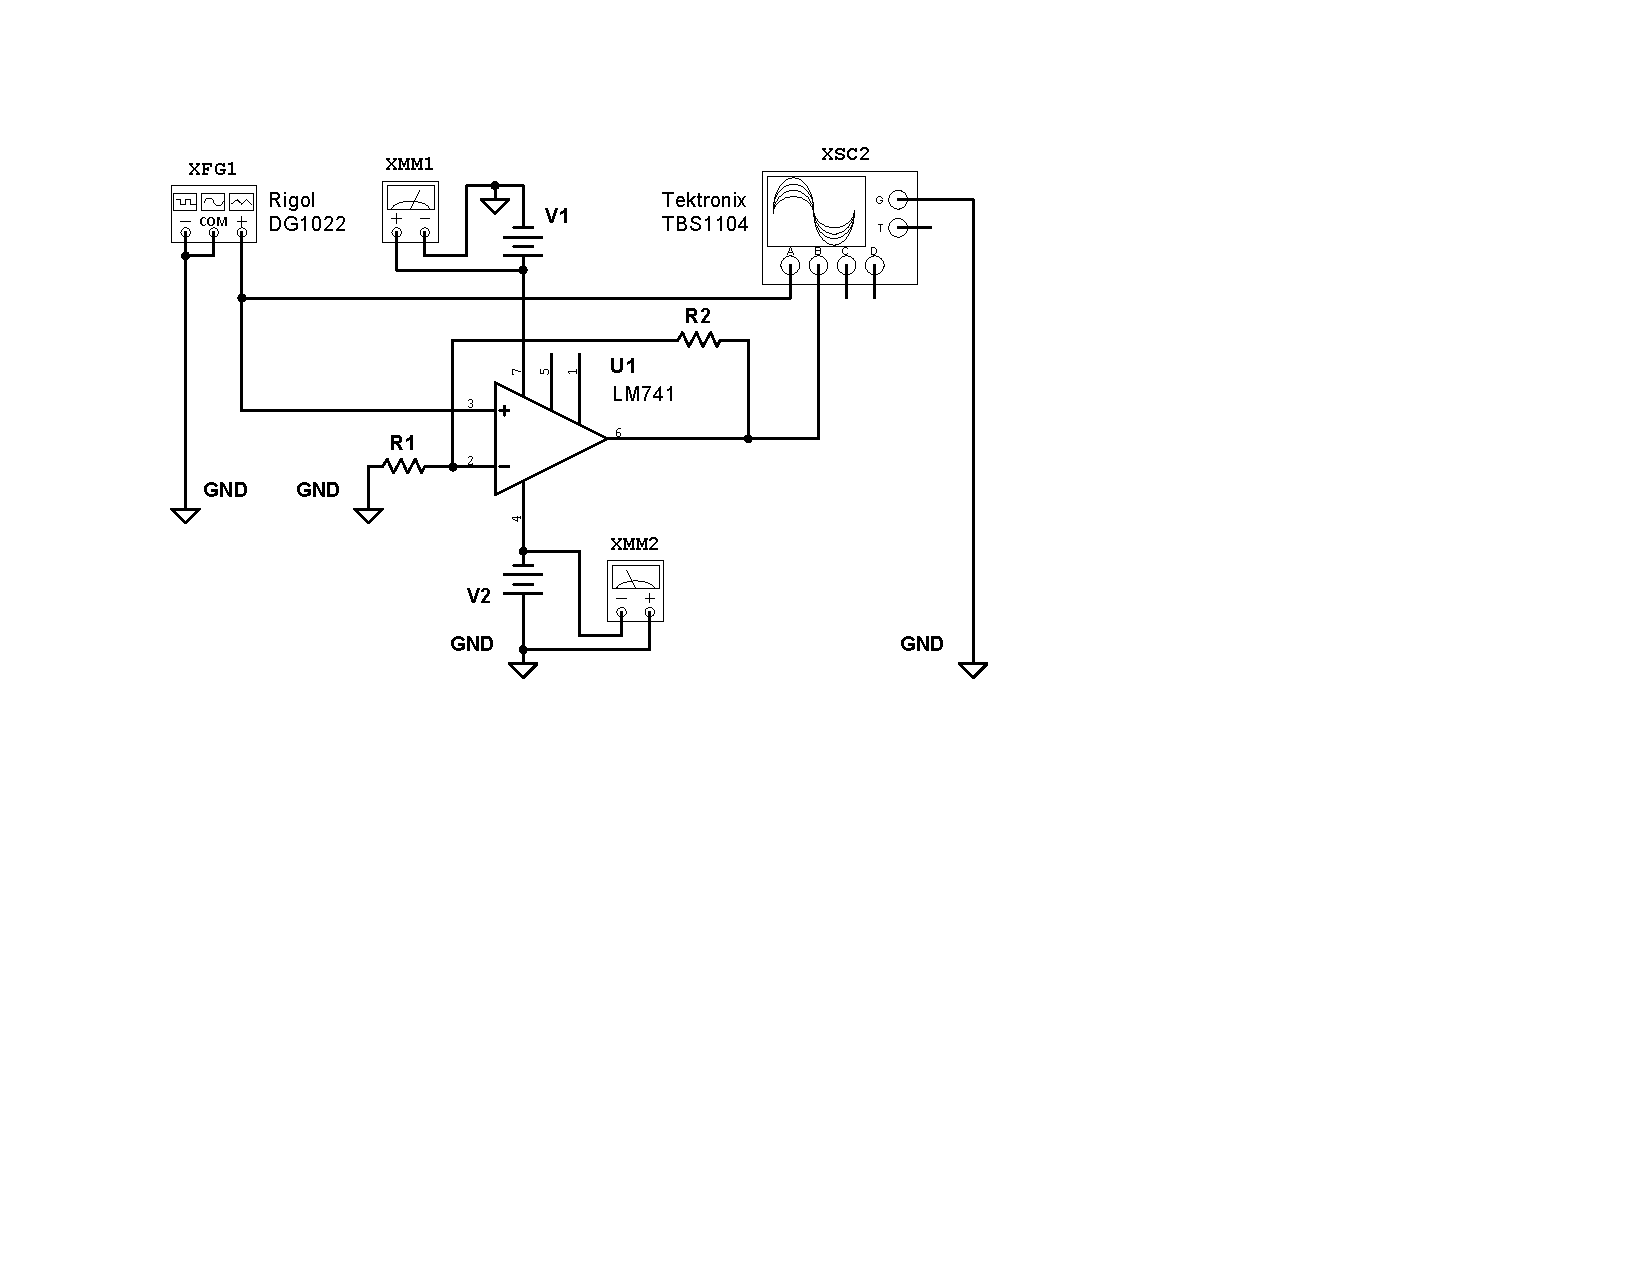
\includegraphics[width=0.48\textwidth]{sch-simulations/output/OPA-closed-loop-non-inverting.pdf}
\caption{Schema del circuito elettrico per la caratterizzazione dell'OPA retroazionato non invertente. Valori per i componenti utilizzati misurati con il multimetro: R1 = ( $987 \pm 14$ ) $\Omega$ , R2 = ( $990 \pm 14$ ) $\Omega$
\\}
\label{fig:loop-non-inv}
\end {center}
\end{figure}

\vspace{-2mm}

Un amplificatore non invertente ha la peculiarità di dare in uscita un segnale proporzionale a quello d'ingresso e in fase con esso. Il segnale è applicato all'ingresso non invertente affinché il guadagno $A$ sia positivo. Infatti per l'equipotenzialità degli ingressi si ha: 

\vspace{-3mm}

\begin{equation}
    V_{-} = V_{+} = V_{i} = \frac{R_1}{R_1+R_2}
\end{equation}
\begin{equation}
    [V_{o}=(1+\frac{R_2}{R_1}V_{+})
\end{equation}
\begin{equation}
    A=\frac{V_{o}}{V_i}=1+\frac{R_2}{R_1}
\end{equation}
\vspace{-7mm}

\subsection{\textbf{Caratterizzazione}}



\begin{figure}[H]%[!ht]

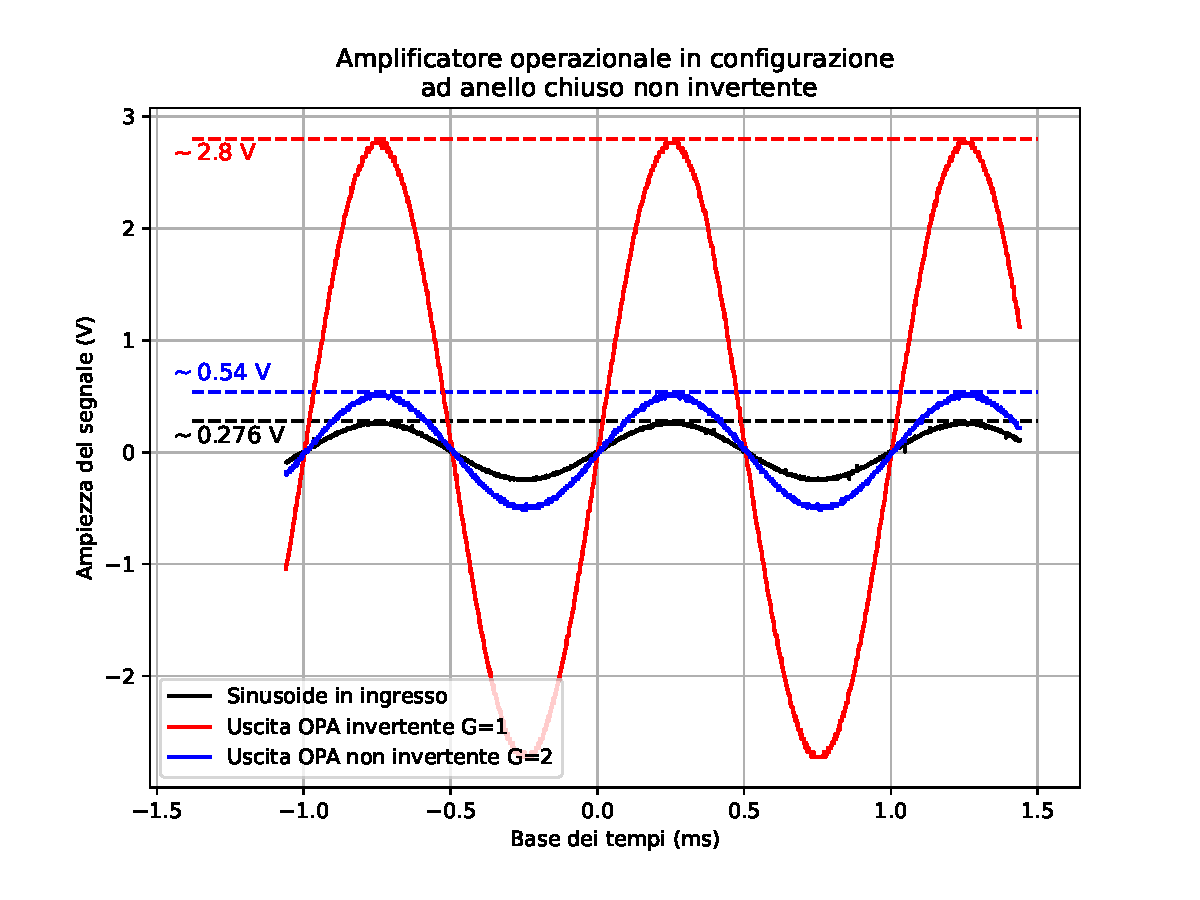
\includegraphics[width=0.48\textwidth]{analysis/output/OPA-closed-loop-non-inv-G2-11.pdf}
\caption{Amplificatore operazionale in configurazione ad anello chiuso non invertente (curva di colore blu)}
\label{fig:g2-11}

\end{figure}

In laboratorio si è considerata la configurazione citata in \textit{Fig.\ref{fig:loop-non-inv}} con l'obiettivo di ottenere un guadagno teorico A = 2. In dettaglio, sfruttando la legge sopracitata
\[A_2 = 1 + R_2/R_1 = 2.003 \pm 0.072\]
\[V_i = (0.276 \pm 0.002) V \: \: V_2 = (0.54 \pm 0.01) V\]

Dalla \textit{Fig. \ref{fig:g2-11}} si nota infatti che la risposta del circuito conferma il comportamento atteso, osserviamo, infatti, un segnale in uscita in fase con quello in entrata, con un guadagno $A_{2_c} = 1.96 \pm 0.05$. L'accordo tra il guadagno atteso e quello misurato sperimentalmente con l'oscilloscopio è confermato da un \textit{Test Z} che riporta il seguente valore per la variabile statistica $Z = 0.54$, minore del valore di Z critico corrispondente ad un livello di significatività del 5 \%.


\subsection{\textbf{Studio della risposta in frequenza}}

\vspace{-20mm}

\begin{figure}[H]%[!ht]
\begin {center}
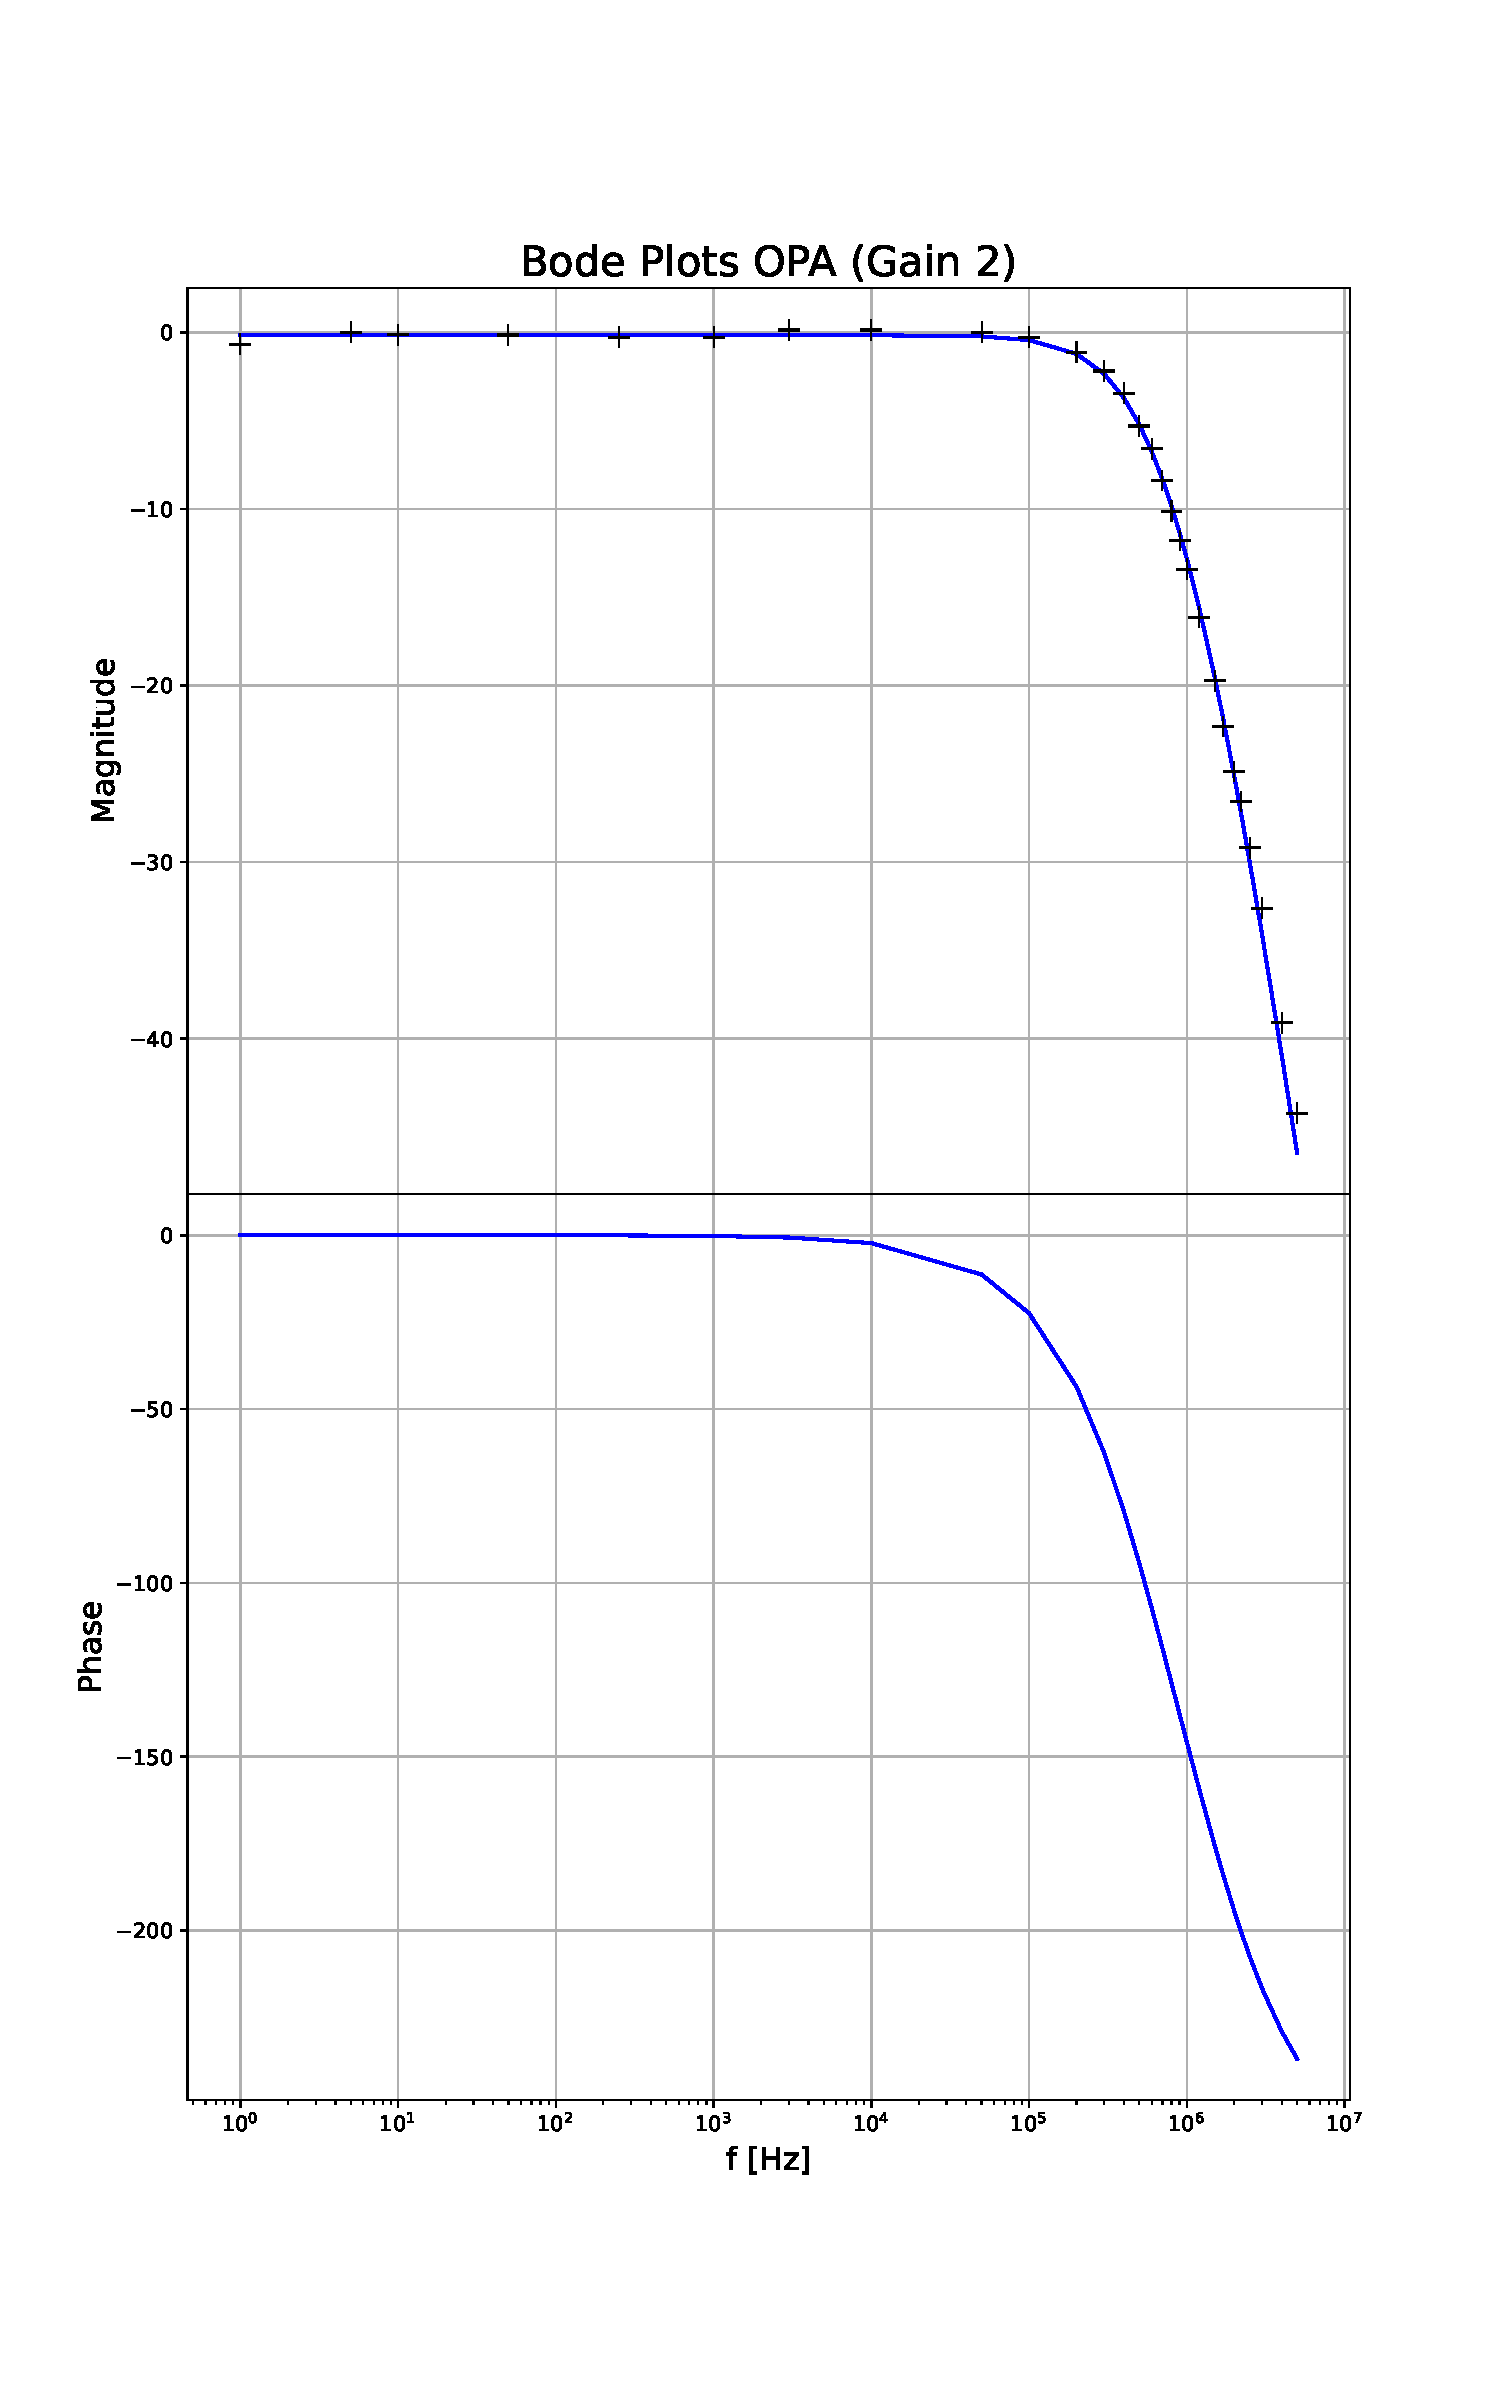
\includegraphics[width=0.50\textwidth]{analysis/output/OPA-bode_gain2(mag+phase).pdf}
\vspace{-8mm}
\caption{Diagramma di Bode con OpAmp non invertente}
\label{fig:gain2}
\end{center}
\end{figure}


Si è ora interessati a valutare la risposta in frequenza del circuito di amplificazione sotto esame, vengono quindi acquisiti i valori picco-picco dell'ingresso e dell'uscita con gli strumenti di misura automatica dell'oscilloscopio (i dati sono riportati nella \textit{tabella \ref{tab:opa-non-inv}}). I punti sul piano \textit{guadagno-frequenza} vengono interpolati con una opportuna funzione di trasferimento del circuito, espressa in trasformata di Laplace nella forma seguente:

\begin{equation}
    H(s)=\frac{k}{(1+as)}
\end{equation}

in cui $k$ rappresenta il guadagno e $a = \frac{1}{f_H}$ con $f_H$ la frequenza di taglio. 

Nel grafico in \textit{Fig. \ref{fig:gain2}} è riportato in primo luogo il diagramma di Bode relativo all'ampiezza, ottenuto per mezzo della regressione di $H(s)$. In quest'ultimo la $f_{H_2}$ ($f_{H}$ con A = 2) è stata ricavata dall'intersezione tra la curva di fit e un cursore orizzontale ad altezza pari al guadagno nella regione di \textit{plateau} sottratto di $3$ $dB$. Il diagramma di fase è stato ricavato dalla funzione di trasferimento e vi sono stati sovrapposti i valori acquisiti con l'oscilloscopio. 

\subsection{\textbf{Slew rate}}

\begin{figure}[H]%[!ht]
\begin {center}
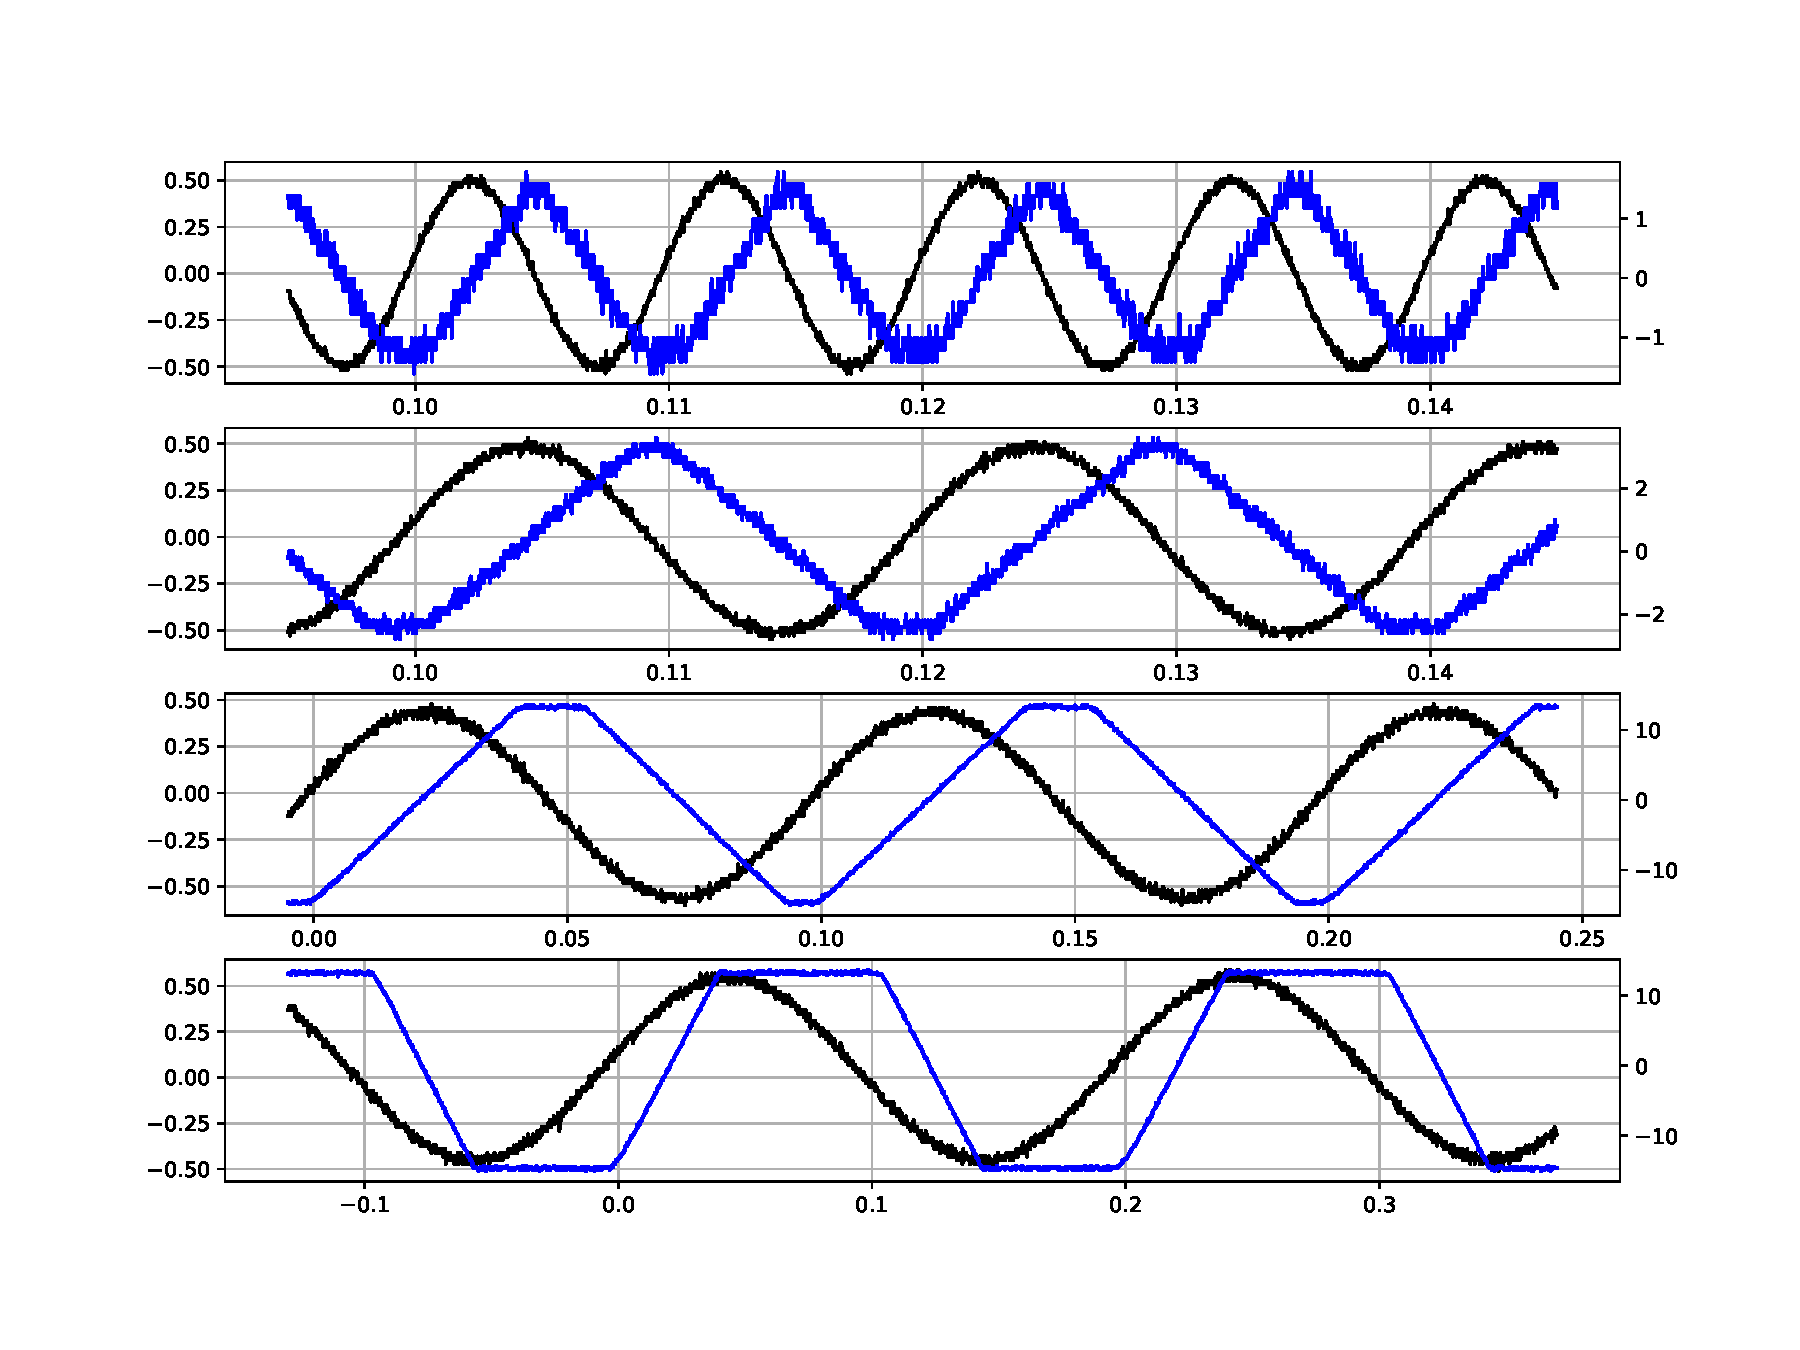
\includegraphics[width=0.50\textwidth]{analysis/output/OPA-open-loop-slew-rate.pdf}
\caption{Amplificazione ad anello aperto al variare della frequenza, dall'alto f = 100, 50, 10, 5 kHz}
\label{fig:slew-rate-table}
\end {center}
\end{figure}


In un amplificatore operazionale reale la velocità di variazione della tensione di uscita non può superare un valore limite detto \textit{slew-rate} o velocità di risposta:
\begin{equation}
    SR = (\frac{dV_{out}}{dt})_{max}
\end{equation}

Per il dispositivo LM741 il datasheet riporta un valore pari a 0.5 V/$\mu$s a T = 298 K.
Questa limitazione è dovuta a fenomeni non lineari quali la saturazione dello stadio di ingresso dell'amplificatore operazionale e non è in relazione con la larghezza di banda finita dell'OPA. 
Per analizzare tale fenomeno è stata nuovamente realizzata la configurazione ad anello aperto ed è stata osservata la risposta del circuito all'aumento progressivo della frequenza del segnale in ingresso da amplificare, con valori di tensione picco-picco elevati ($V_{pp}$ = 1 V). Raggiunta la frequenza di 100 kHz si è potuto osservare come i fronti di salita e discesa in uscita dall'OPA nel punto in cui è attesa la massima variazione fossero approssimabili con una retta con coefficiente angolare corrispondente allo slew-rate. E' quindi stato possibile valutare quantitativamente questa caratteristica, confrontandola con quanto espresso sul datasheet del produttore, mediante una regressione lineare.


\begin{figure}[H]%[!ht]
\begin {center}
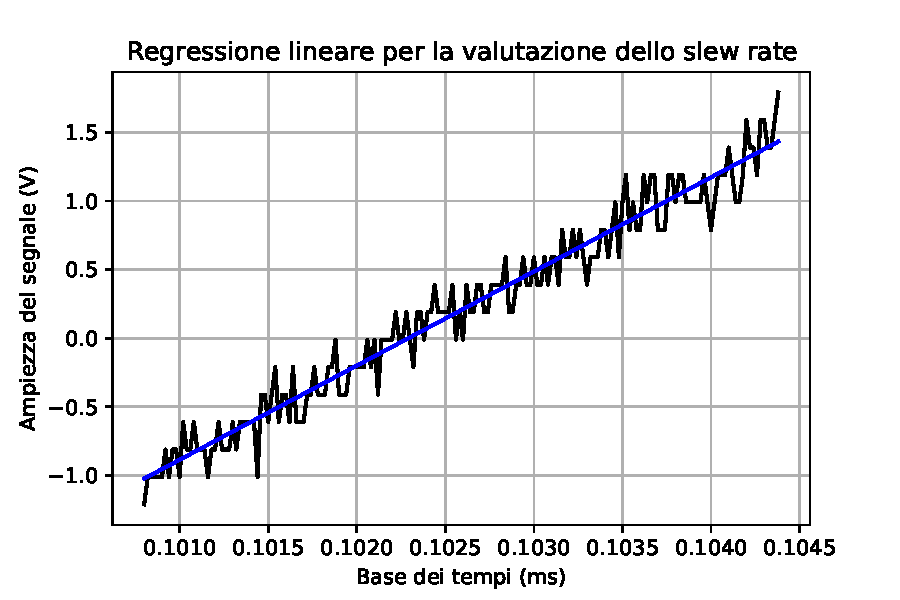
\includegraphics[trim = {30pt 0 0 0}, width=0.53\textwidth]{analysis/output/OPA-slew-rate-fit.pdf}
\caption{Regressione lineare effettuata sul fronte di salita del segnale di output a 100 kHz, riferimento alla \textit{Fig. \ref{fig:slew-rate-table}}}
\label{fig:slew-rate-fit}
\end {center}
\end{figure}


Il valore del coefficiente angolare della retta restituito da minimizzatore ci porta a concludere che SR = $(0.7 \pm 0.1) \frac{V}{\mu s}$, valore compatibile con quanto riportato nel datasheet, infatti un test Z eseguito attribuendo al valore teorico un'incertezza pari all'ultima cifra significativa restituisce una variabile statistica Z = 1.43 $<$ $Z_{c}$ = 1.96 con $\alpha$ = 5 \%.

\subsection{\textbf{Discussione e conclusioni}}
In conclusione il circuito ha dimostrato di operare esattamente come previsto, processando un segnale in output in fase con quello in input, e amplificato di un valore consistente con quello calcolato per via teorica. La funzione di trasferimento impiegata si è dimostrata perfettamente in linea con i dati sperimentali, sia per quanto riguarda le misure di fase, che per le misure di ampiezza. Notiamo però, che mentre le misure di ampiezza sono risultate sufficientemente accurate, l'oscilloscopio è risultato impreciso nel misurare lo sfasamento. Infine lo slew-rate estratto dalla regressione è risultato in accordo con quanto riportato sul datasheet.

%%%%%%%%%%%%%%%%%%%%%%%%%%%%%%%%%%%%%%%%%%
\section{\textbf{Amplificatore retroazionato invertente}} %Stefano

\subsection{\textbf{Introduzione}}

\begin{figure}[H]%[!ht]
\begin {center}
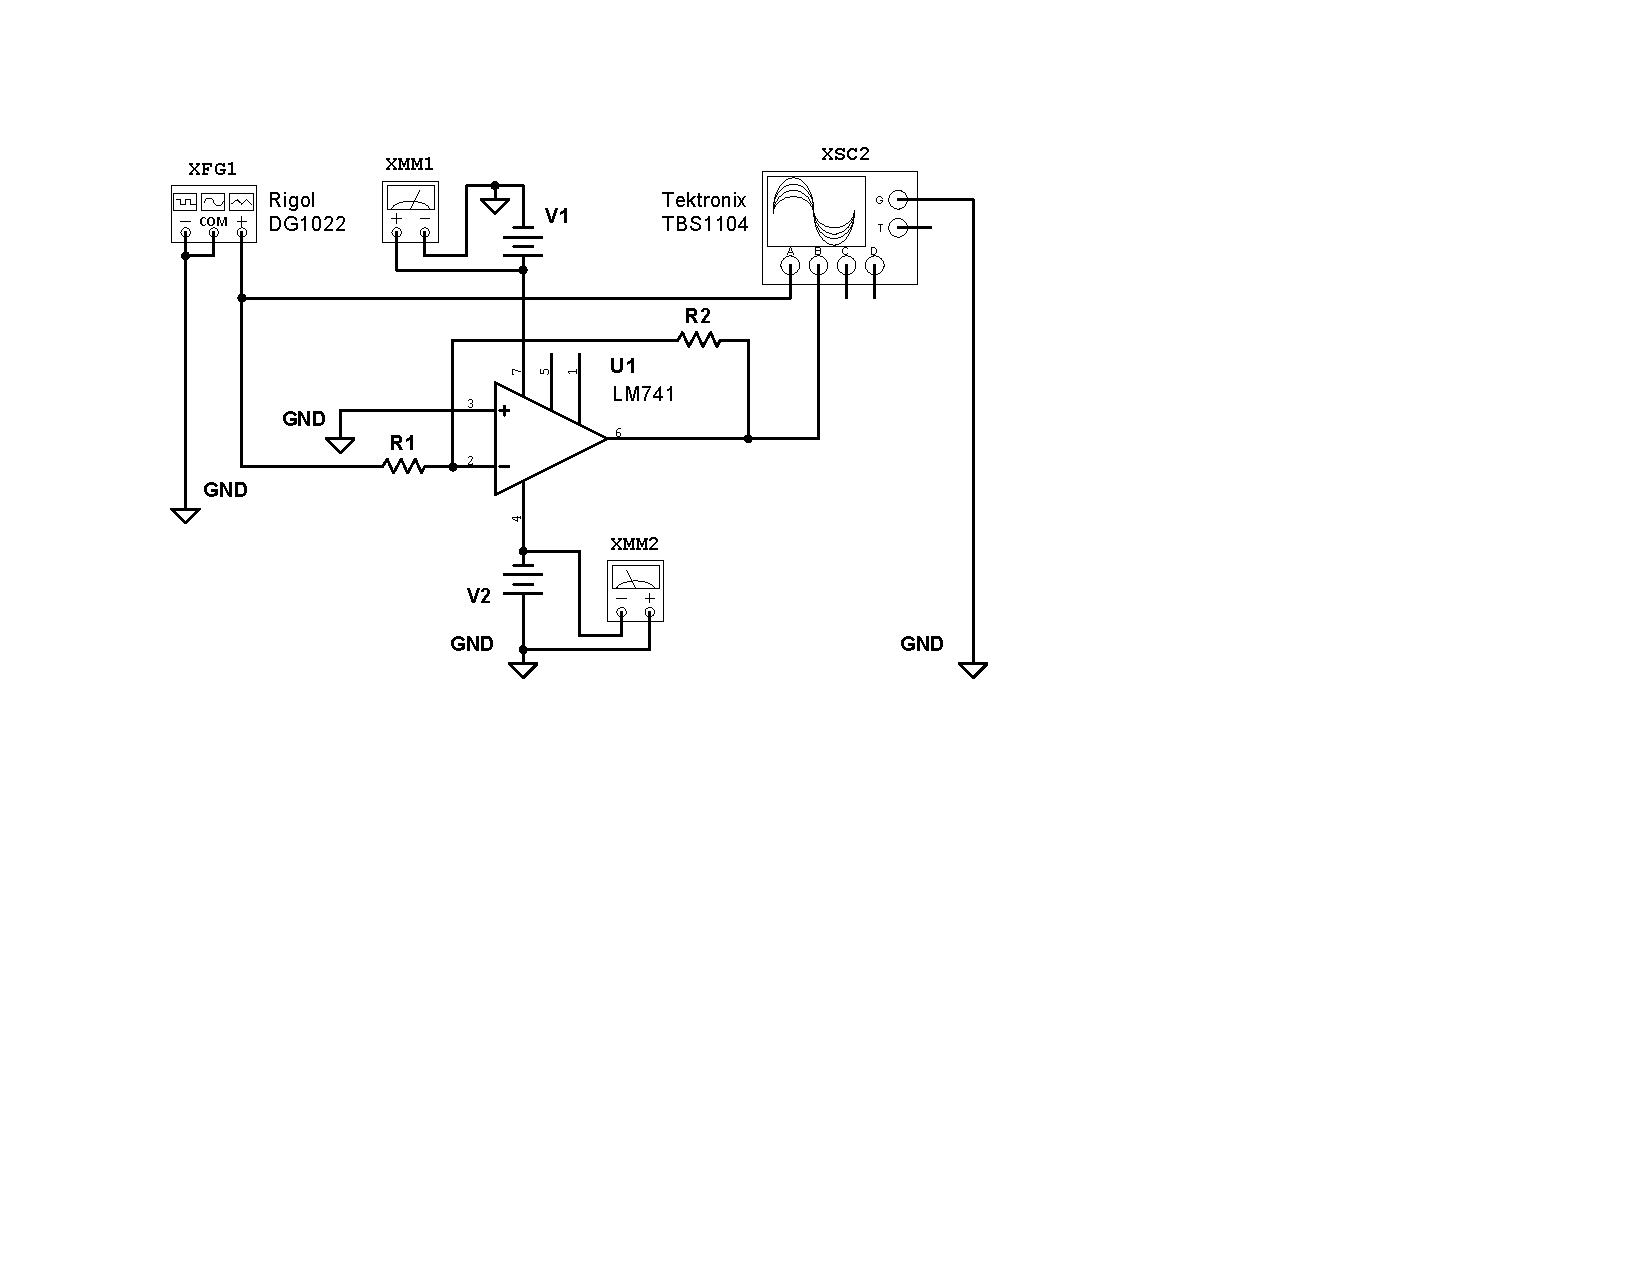
\includegraphics[width=0.38\textwidth]{sch-simulations/output/OPA-closed-loop-inverting.pdf}
\caption{Amplificatore retroazionato invertente: $R_2$ è la resistenza di feedback.}
\label{fig:circ_closed_loop_inv}
\end {center}
\end{figure}

Dopo aver analizzato nel dettaglio il circuito amplificatore retroazionato non invertente, si ripete ora parte dell'analisi in configurazione invertente.

Il comportamento atteso da tale configurazione prevede che il guadagno sia pari a $A_{vf} = -\frac{R_2}{R}$. 
Ci si propone di studiare l'andamento in frequenza dell'amplificazione in due diversi casi: guadagno teorico pari a $-1$ e guadagno teorico pari a $-10$.

Per il primo caso si utilizzano due resistori $R_2 = 1.00 \pm 0.01 k\Omega $ e $R = 0.99 \pm 0.01 k\Omega$, con guadagno teorico pari a $A_{vf} = -1.00 \pm 0.02 $ Per il secondo caso si utilizzano due resistori $R_2 = 0.99 \pm 0.01 k\Omega $ e $R = 0.99 \pm 0.01 k\Omega$, con guadagno teorico pari a $A_{vf} = -9.8 \pm 0.2$

Come segnale in ingresso si è scelta un'onda di tipo sinusoidale, con ampiezza di $100 mV$.

I dati misurati sono riportati nelle \textit{tabelle \ref{tab:opa-inv-g1} (guadagno 1) e \ref{tab:opa-inv-g10} (guadagno 10)}

\subsection{\textbf{Studio della risposta in frequenza}}

Sono stati acquisiti valori di guadagno nell'intervallo di frequenze da 0 a 5 MHz e sono stati interpolati con una funzione di trasferimento $H(s)$ in modo analogo al caso della configurazione non invertente: 

\begin{equation}
    H(s) = \frac{k}{1+as}
\end{equation}

Il minimizzatore ha restituito per i parametri i valori $k = -R_2/R$ e $a = \frac{1}{f_H}$. Da questa funzione è stato possibile stimare il guadagno - $3 dB$, e tramite un cursore orizzontale posto a tale livello si è trovata l'intersezione con la curva teorica, corrispondente alla frequenza di taglio $f_H$.

\begin{figure}[H]%[!ht]
\begin{center}
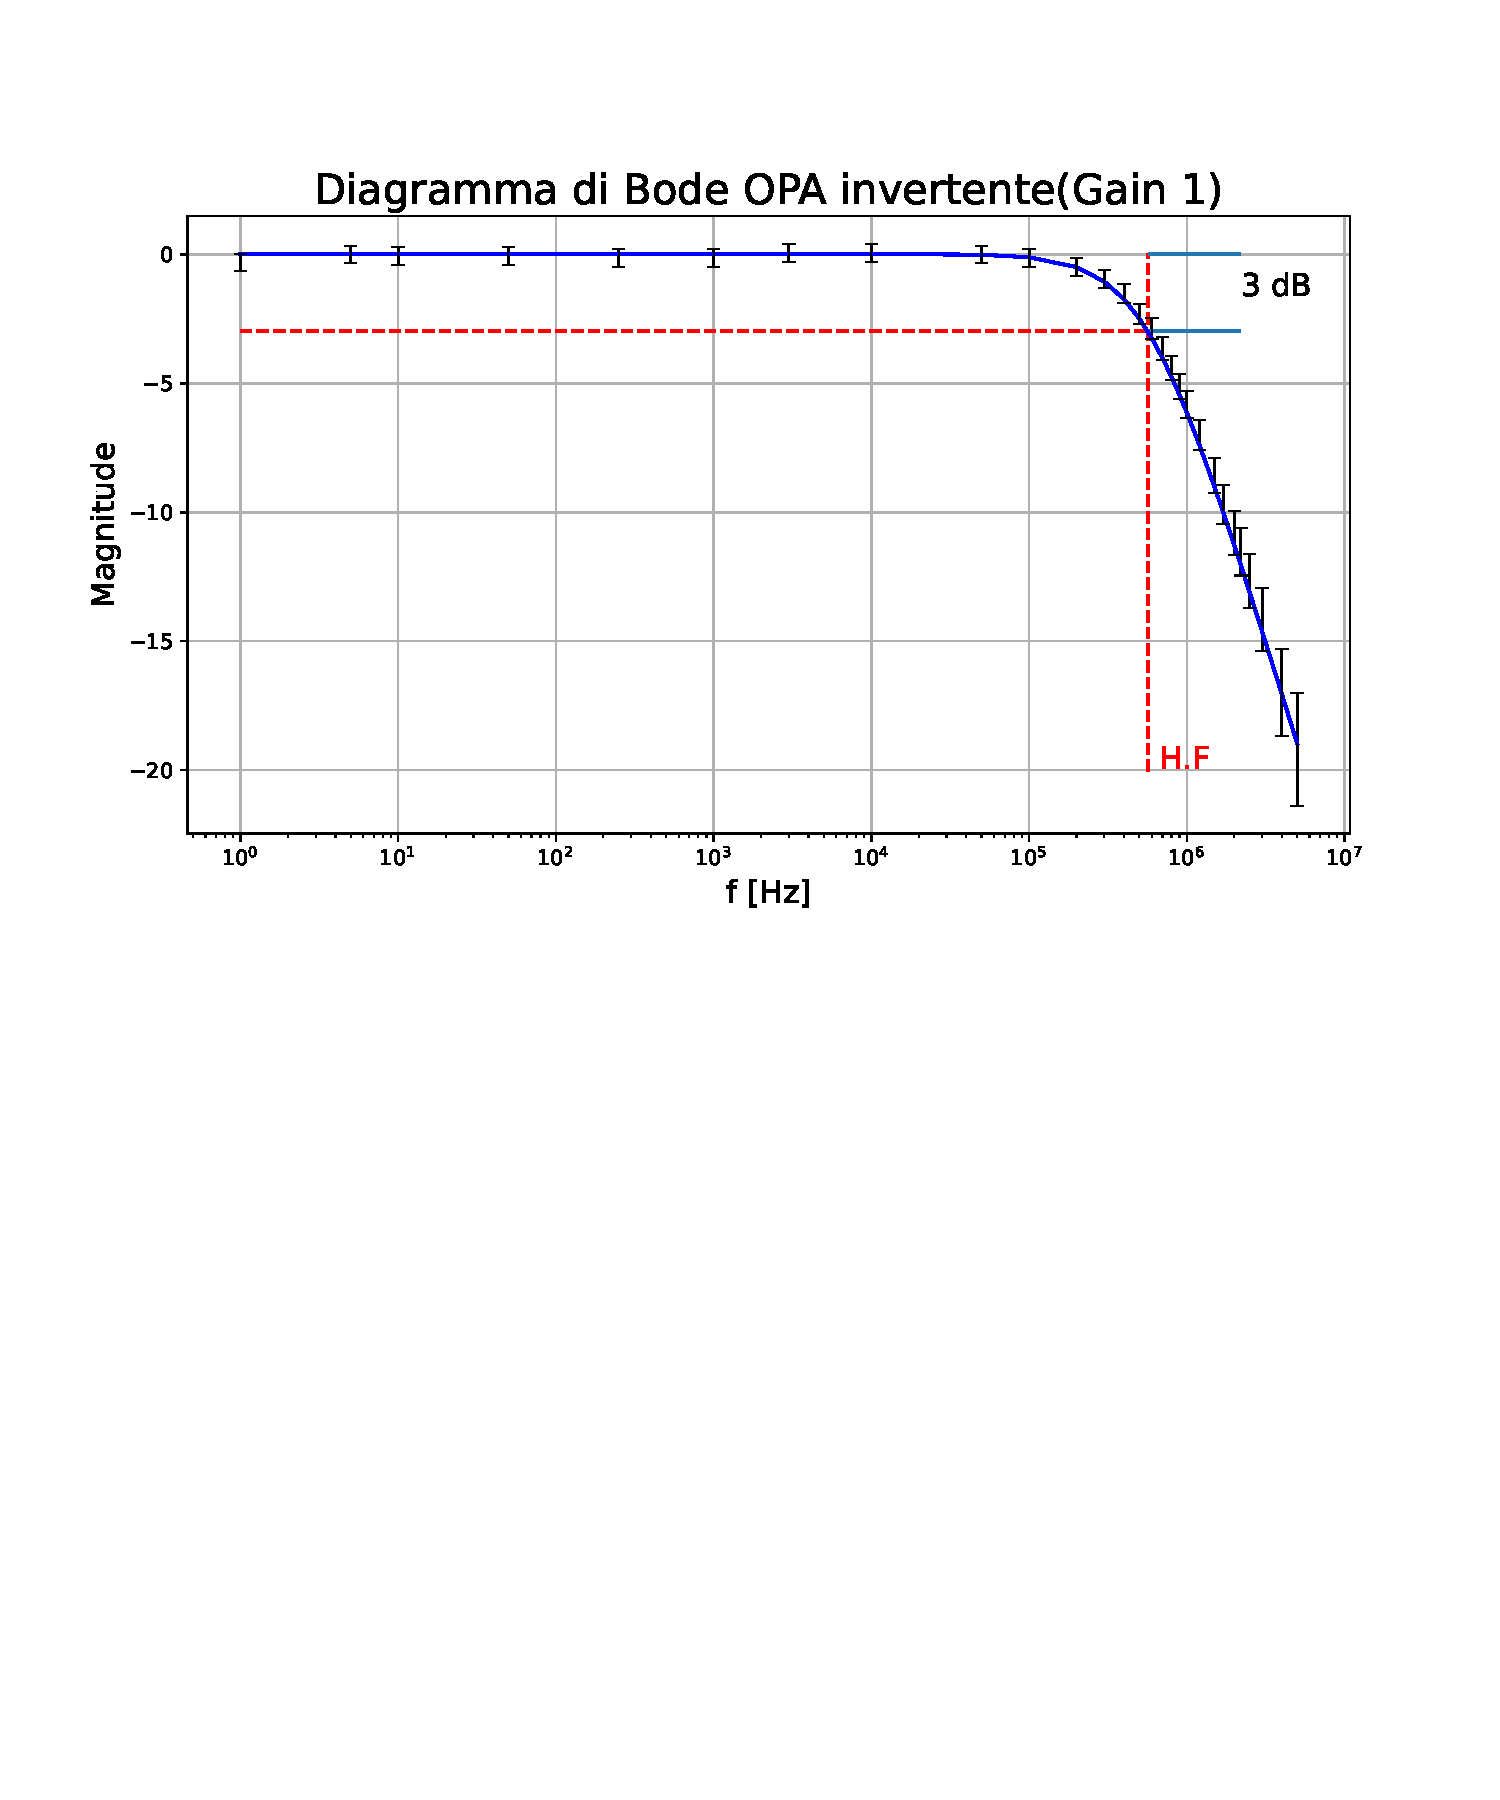
\includegraphics[width=0.48\textwidth]{analysis/output/OPA-bode_gain1(mag).pdf}
\caption{Amplificatore retroazionato invertente con guadagno teorico 1: risposta in funzione della frequenza. In rosso il cursore a livello $f_H$}
\label{fig:closed_loop_inv_gain_1}
\end{center}
\end{figure}

Per il caso con guadagno teorico 1 il test di adattamento della variabile $\chi^2$ = 7.31 ha restituito un p-value pari a 0.99.
Dal fit si sono ricavati i seguenti parametri:
$A_{fit} = 0.0264 \pm 0.001 dB$
$f_{H1} = (0.57 \pm 0.03) MHz$
$k_1 = 1.0 \pm 0.1$

\begin{figure}[H]%[!ht]
\begin {center}
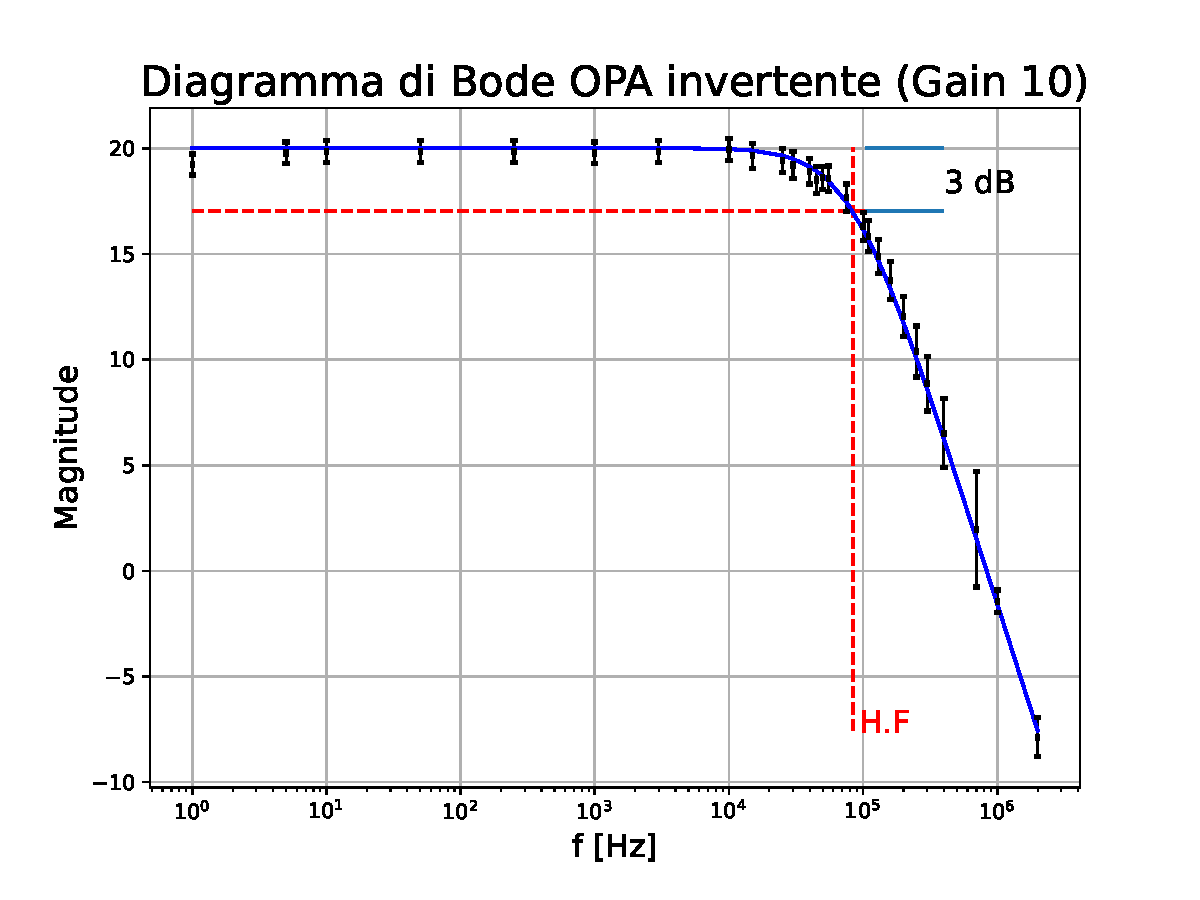
\includegraphics[width=0.48\textwidth]{analysis/output/OPA-bode_gain10(mag).pdf}
\caption{Amplificatore retroazionato invertente con guadagno teorico 10: risposta in funzione della frequenza. In rosso il cursore a livello $f_H$ }
\label{fig:closed_loop_inv_gain_10}
\end {center}
\end{figure}

%\vfill

Per il caso con guadagno teorico 10 il test di adattamento della variabile $\chi^2$ = 5.55 ha restituito un p-value pari a 0.99.
Dal fit si sono ricavati i parametri:
$A_{fit} = 20.026 \pm 0.001$ $dB$
$f_{H10} = (0.84 \pm 0.05)$ $MHz$.
$k_{10} = 9.6 \pm 0.1$

\subsection{\textbf{Studio della conservazione del prodotto guadagno x larghezza di banda}}

E' noto che in un circuito amplificatore realizzato con amplificatori operazionali in prodotto guadagno x larghezza di banda è una caratteristica costante del dispositivo. Si è quindi voluta valutare la compatibilità tra quanto ottenuto nel caso con guadagno A = 10 e A = 1: $\\ | BW \times A_1 | = (0.56 \pm 0.03)\ MHz \\$  e  $ | BW \times A_{10} | = (0.84 \pm 0.05)\ MHz$
Questa volta, contrariamente a quanto atteso, un test statistico tra i due prodotti $BW \times A$ sfruttando i valori di $f_H$ e $k$ estratti per regressione non ha dato risultati consistenti entro un livello di significatività del 5\% ($Z = 4.83 > Z_c = 1.96$). I risultati sono però comunque all'interno del range atteso 0.431 - 1.5 MHz riportato sul datasheet. Notiamo che il prodotto con valore più basso è quello ricavato a frequenza più alta, questo ci permette di ipotizzare che ad alta frequenza qualche fenomeno che necessita di ulteriori misure per essere giustificato correttamente abbia alterato i valori di guadagno misurati portando ad una sottostima della frequenza di taglio.
Anche dal grafico in figura \ref{fig:OPA-bode_gain_comparison(mag)} si nota, infatti, che ad alte frequenze le due funzioni di trasferimento ottenute per fit non tendono a sovrapporsi come sarebbe atteso.


\begin{figure}[H]%[!ht]
\begin {center}
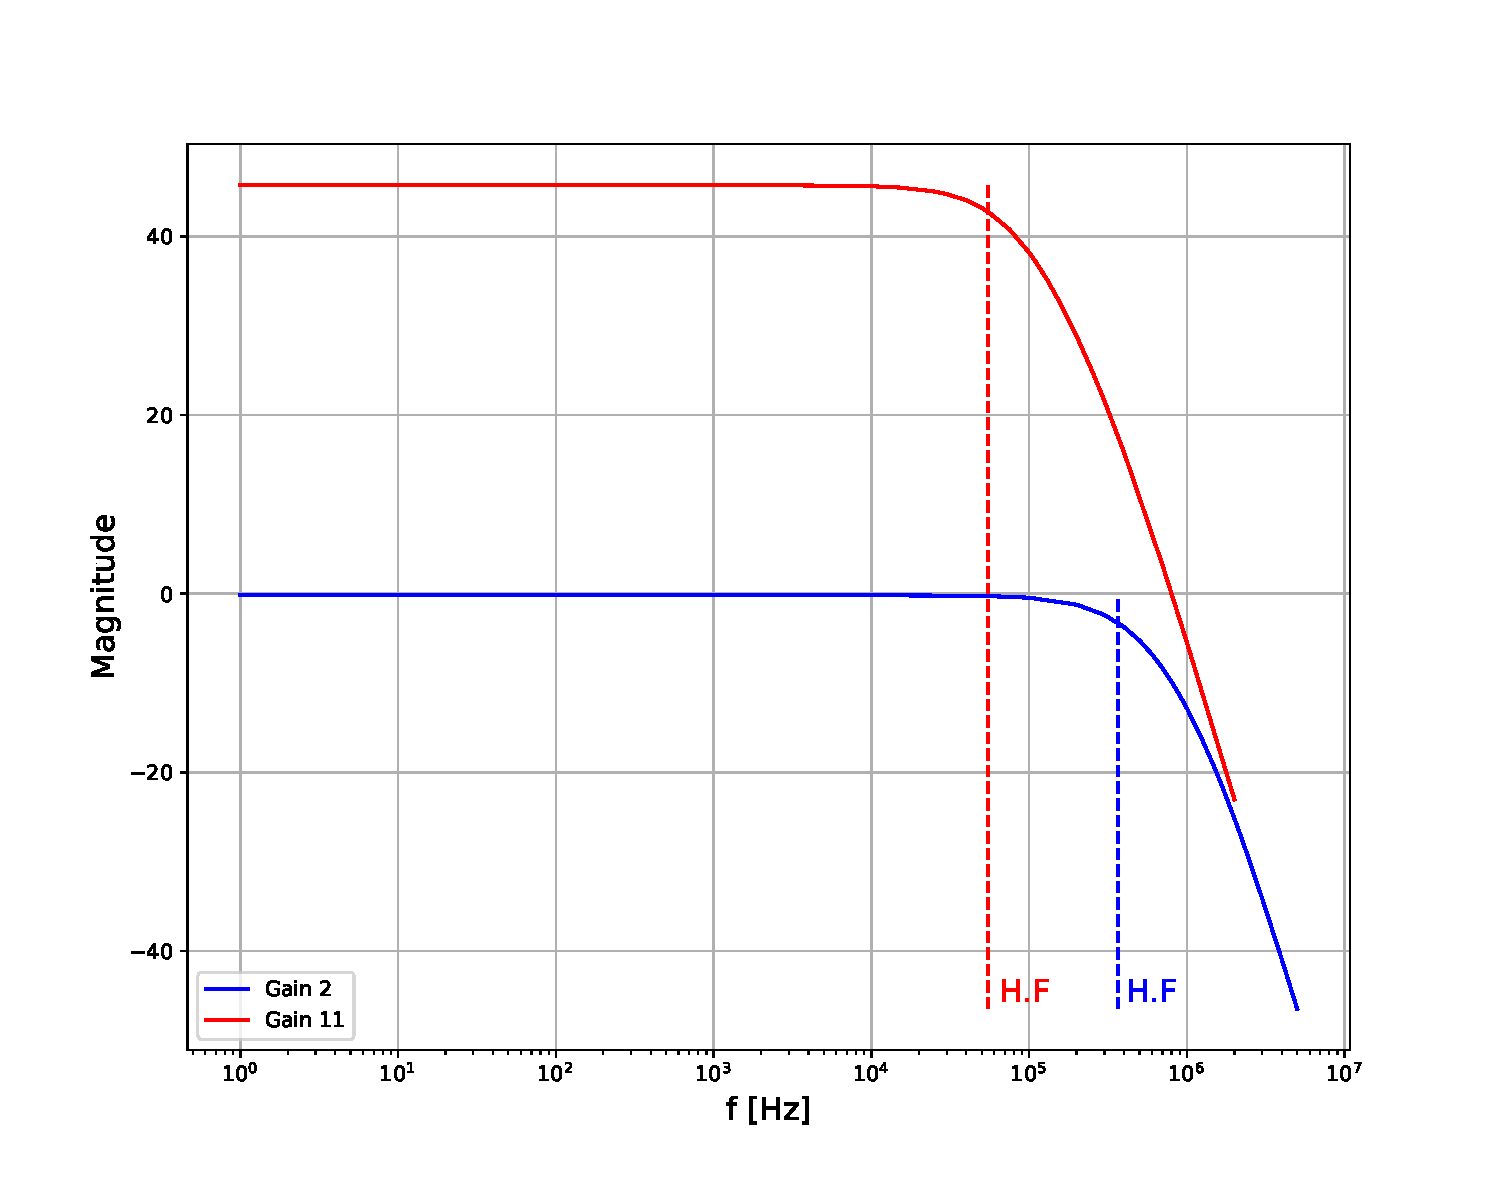
\includegraphics[width=0.48\textwidth]{analysis/output/OPA-bode_gain_comparison(mag).pdf}
\caption{Confronto tra guadagno e larghezza di banda}
\label{fig:OPA-bode_gain_comparison(mag)}
\end {center}
\end{figure}

%%%%%%%%%%FINE PRIMO GIORNO%%%%%%%%%%%%%%%
%%%%%%%%%%INIZIO SECONDO GIORNO%%%%%%%%%%%

%%%%%%%%%%%%%%%%%%%%%%%%%%%%%%%%%%%%%%%%%%
\section{\textbf{Amplificatore logaritmico}} %Stefano
\subsection{\textbf{Introduzione all'esperienza}}
Un amplificatore operazionale, se inserito in un circuito che usa un diodo nella rete di feedback, amplifica il segnale in ingresso secondo la legge

\begin{equation}
V_0 = - \eta \cdot V_T \cdot ln( \frac{v_s}{R \cdot I_0} )
\end{equation}
con $V_T = \frac{k_{b} \cdot T}{q}$ \\

derivante dalla caratteristica tensione-corrente di Shockey del diodo,  realizzando così un amplificatore logaritmico che è particolarmente utile in tutte quelle applicazioni in cui si devono amplificare, misurare o acquisire segnali che spaziano su un range di ampiezze particolarmente vasto.

\subsection{\textbf{Caratterizzazione}}
Ci si propone di verificare la legge, utilizzando un diodo al silicio ($\eta = 2$), un resistore di limitazione della corrente pari a $R = 2.00 \pm 0.02 \ k\Omega$, e fornendo una tensione continua all'ingresso invertente dell'amplificatore operazionale. Inoltre, si intende ricavare sperimentalmente il valore dei parametri $V_T$ e $I_0$ per regressione.

\begin{figure}[H]%[!ht]
\begin {center}
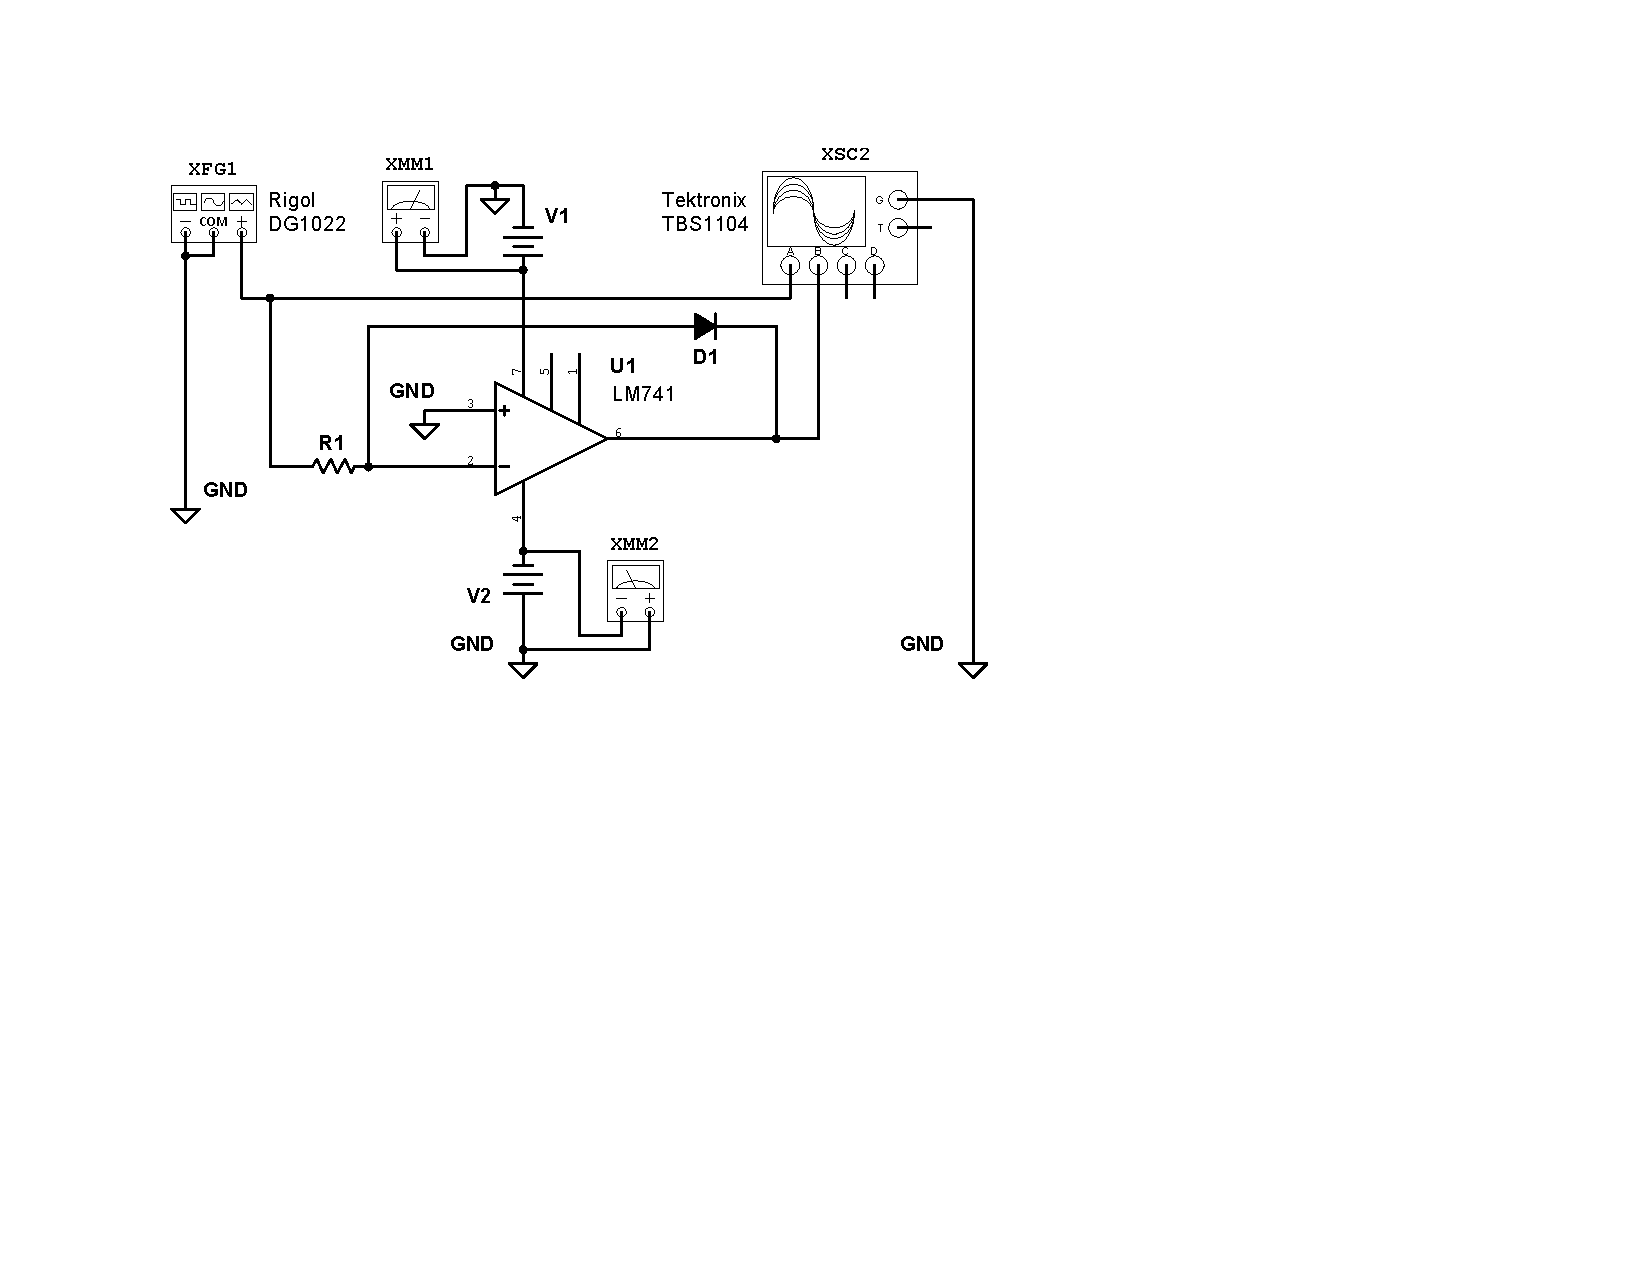
\includegraphics[width=0.38\textwidth]{sch-simulations/output/OPA-log.pdf}
\caption{Circuito per integratore logaritmico. D1 è un diodo al silicio che costituisce la retroazione}
\label{fig:circ_log_ampl}
\end {center}
\end{figure}

Avendo inserito un diodo al silicio la legge può essere riscritta come 

\begin{equation}
V_0 = 2 \cdot V_T \cdot ln(R \cdot I_0) - 2 \cdot V_T \cdot ln(v_s)
\end{equation}

La prima misurazione consiste nell'inviare in ingresso un segnale $V_{in} = 1V$ per ottenere la costante  $V_0 = 2 \cdot V_T \cdot ln(R \cdot I_0)$.
In laboratorio nell'impossibilità con l'alimentatore di fornire un segnale esattamente pari a $1$ V, sono state acquisite alcune misure nell'intorno, che sono poi state mediate.

\begin{center}
\begin{tabular}{|c|c|}
\hline
$V_{in} \pm 0.006 $ [V] & $V_{out} \pm 0.002 [V]$   \\ \hline
1.065 & -0.578 \\ \hline
0.887 & -0.569 \\ \hline
1.099 & -0.578 \\ \hline
0.986 & -0.573 \\ \hline
1.068 & -0.577 \\ \hline
0.966 & -0.572 \\ \hline
\end{tabular}
\end{center}

La media dei valori di $V_{out}$ è risultata pari a 

\[V_{out} = (-0.575 \pm 0.001 )V\]

Si procede dunque allo studio del comportamento dell'amplificatore per valori variabili di tensione in ingresso, volendo ricostruire la legge di Shockley. Le tensioni misurate sono riportate in appendice nella \textit{tabella \ref{tab:opa-log}}.

\begin{figure}[H]%[!ht]
\begin {center}
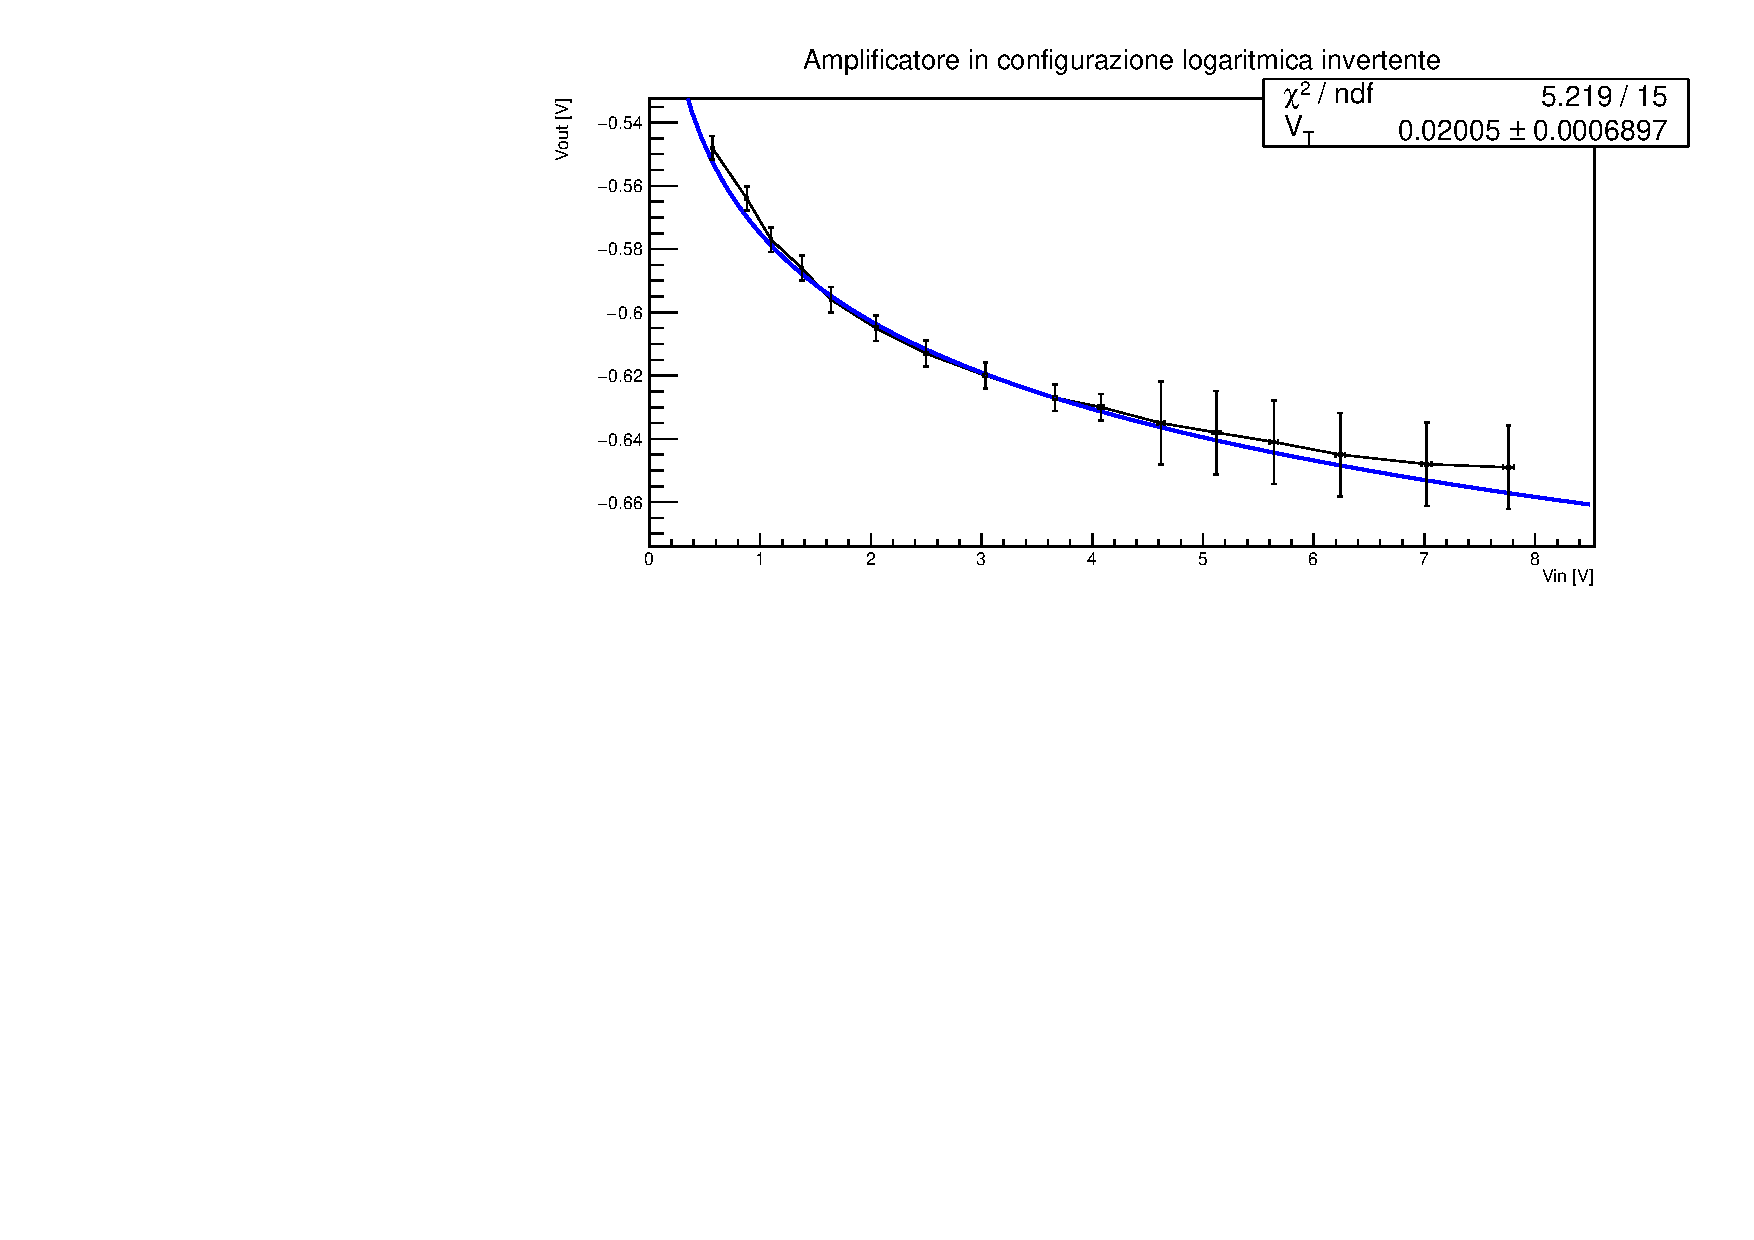
\includegraphics[width=0.48\textwidth]{analysis/output/fit_log_vout_vin.pdf}
\caption{Interpolazione della caratteristica dell'amplificatore logaritmico}
\label{fig:log_ampl_fit}
\end {center}
\end{figure}

Si effettua una regressione tra i valori sperimentali e la funzione teorica 
\begin{equation}
-k - 2 \cdot V_T \cdot ln(v_s)
\end{equation}
con $k = -0.575 \pm 0.001 V$ pari alla costante precedentemente calcolata.

Il $\chi^2$ pari a $5.219$ con 15 gradi di libertà conferma che la funzione teorica descrive con ottima approssimazione i dati misurati, si ottiene infatti un valore del p-value nel test di adattamento di 0.99, superiore al livello di significatività usuale del 5 \%.
La stima del parametro restituisce $V_T =$ $(20.0 \pm 0.7)$ mV, che considerando un valore atteso a temperatura assoluta $T = 300K$ pari a $26 mV$ risulta incompatibile, infatti il test Gauss riporta $Z = 8.637$ evidenziando la presenza di un errore nella stima.

È ragionevole supporre che la temperatura ambiente del laboratorio fosse inferiore a $300 K$, ma non si possiede una misura utile a calcolare un valore atteso più corretto
Si pensa dunque che ci possa essere un errore sistematico nella presa dati, o una sottostima degli errori sulle tensioni in uscita. 

L'ultimo parametro che si intende calcolare è la tensione di saturazione inversa del diodo.
A partire dall'equivalenza $V_0 = 2 \cdot V_T \cdot ln(R \cdot I_0)$  per $v_s = 1$, è possibile sostituire il valore ottenuto di $V_T = 20.0 \pm 0.7 mV$, ottenendo

\[ I_0 = \frac{e^{\frac{k}{2 \cdot V_T}}}{R} = (3 \pm 1) \cdot 10^{-10} A \]

Il valore ha un ordine di grandezza compatibile con la corrente di saturazione inversa attesa, ma si segnala un grande errore relativo ($33 \% $) dovuto alla propagazione degli errori su 3 parametri.


%%%%%%%%%%%%%%%%%%%%%%%%%%%%%%%%%%%%%%%%%%
\subsection{Grafico di risposta e conclusioni}

\begin{figure}[H]%[!ht]
\begin{center}
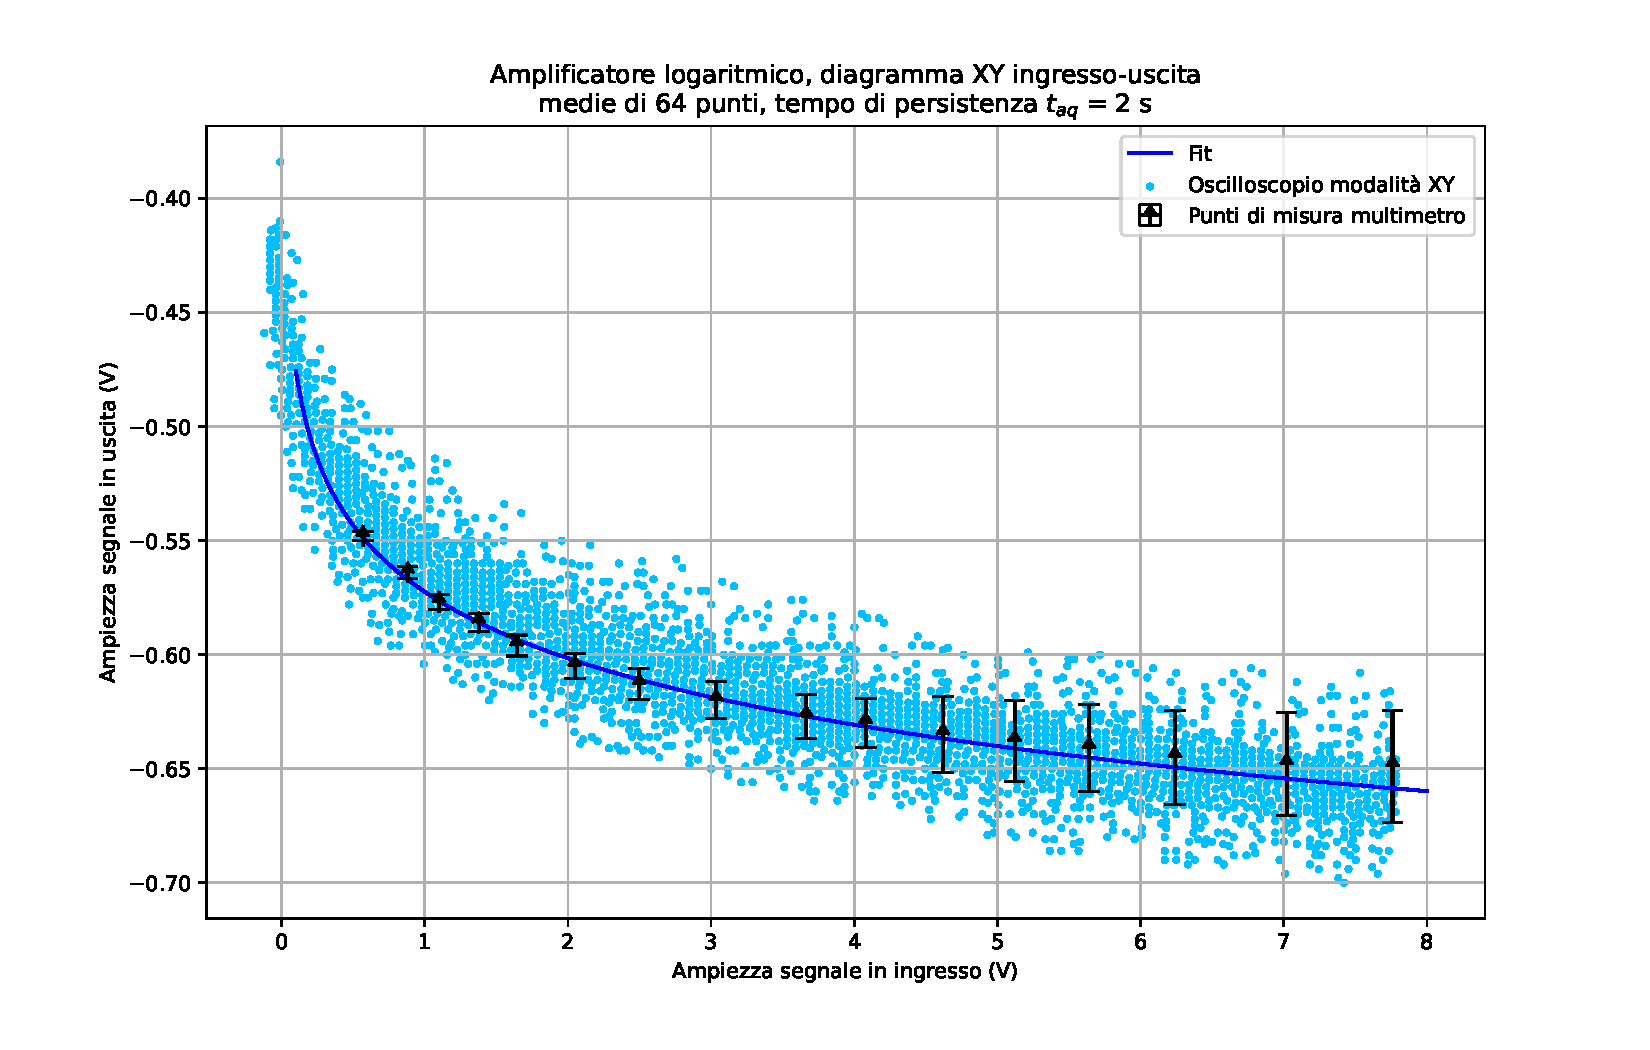
\includegraphics[trim = {10px 0 0 0}, width=0.50\textwidth]{analysis/output/OPA-log-fitted.pdf}
\caption{Caratteristica ingresso-uscita in DC dell'amplificatore logaritmico, in nero i valori misurati con il multimetro, in blu il fit con modello logaritmico, in azzurro la stessa misura effettuata utilizzando l'oscilloscopio in modalità XY}
\label{fig:log_ampl_fit_xy}
\end{center}
\end{figure}

Utilizzando l'oscilloscopio in modalità x-y, con persistenza infinita dei dati, e inviando in ingresso un segnale sinusoidale alla frequenza di $1 Hz$, si è ottenuta una distribuzione di valori di $V_{out}$. In figura \ref{fig:log_ampl_fit_xy} si può notare come la curva dei dati sperimentali con fit rientri all'interno di questo range, ma si trovi vicino ad un estremo per valori bassi di tensione in ingresso.
Questa valutazione sostiene l'ipotesi di un errore sistematico nella presa dati, risultante in una stima imprecisa dei parametri del fit.


%%%%%%%%%%%%%%%%%%%%%%%%%%%%%%%%%%%%%%%%%%
\section{\textbf{Amplificatore integratore invertente}} %Matteo

In questa esperienza di laboratorio verrà analizzato il funzionamento di un circuito integratore attivo realizzato mediante un amplificatore operazionale, osservandone in primo luogo la risposta a diversi tipi di segnali, quali a gradino, rampa e sinusoidali, per poi studiarne il comportamento in funzione della variazione di frequenza della $V_{in}$.
\subsection{\textbf{Circuito}}
\begin{figure}[H]%[!ht]
\begin{center}
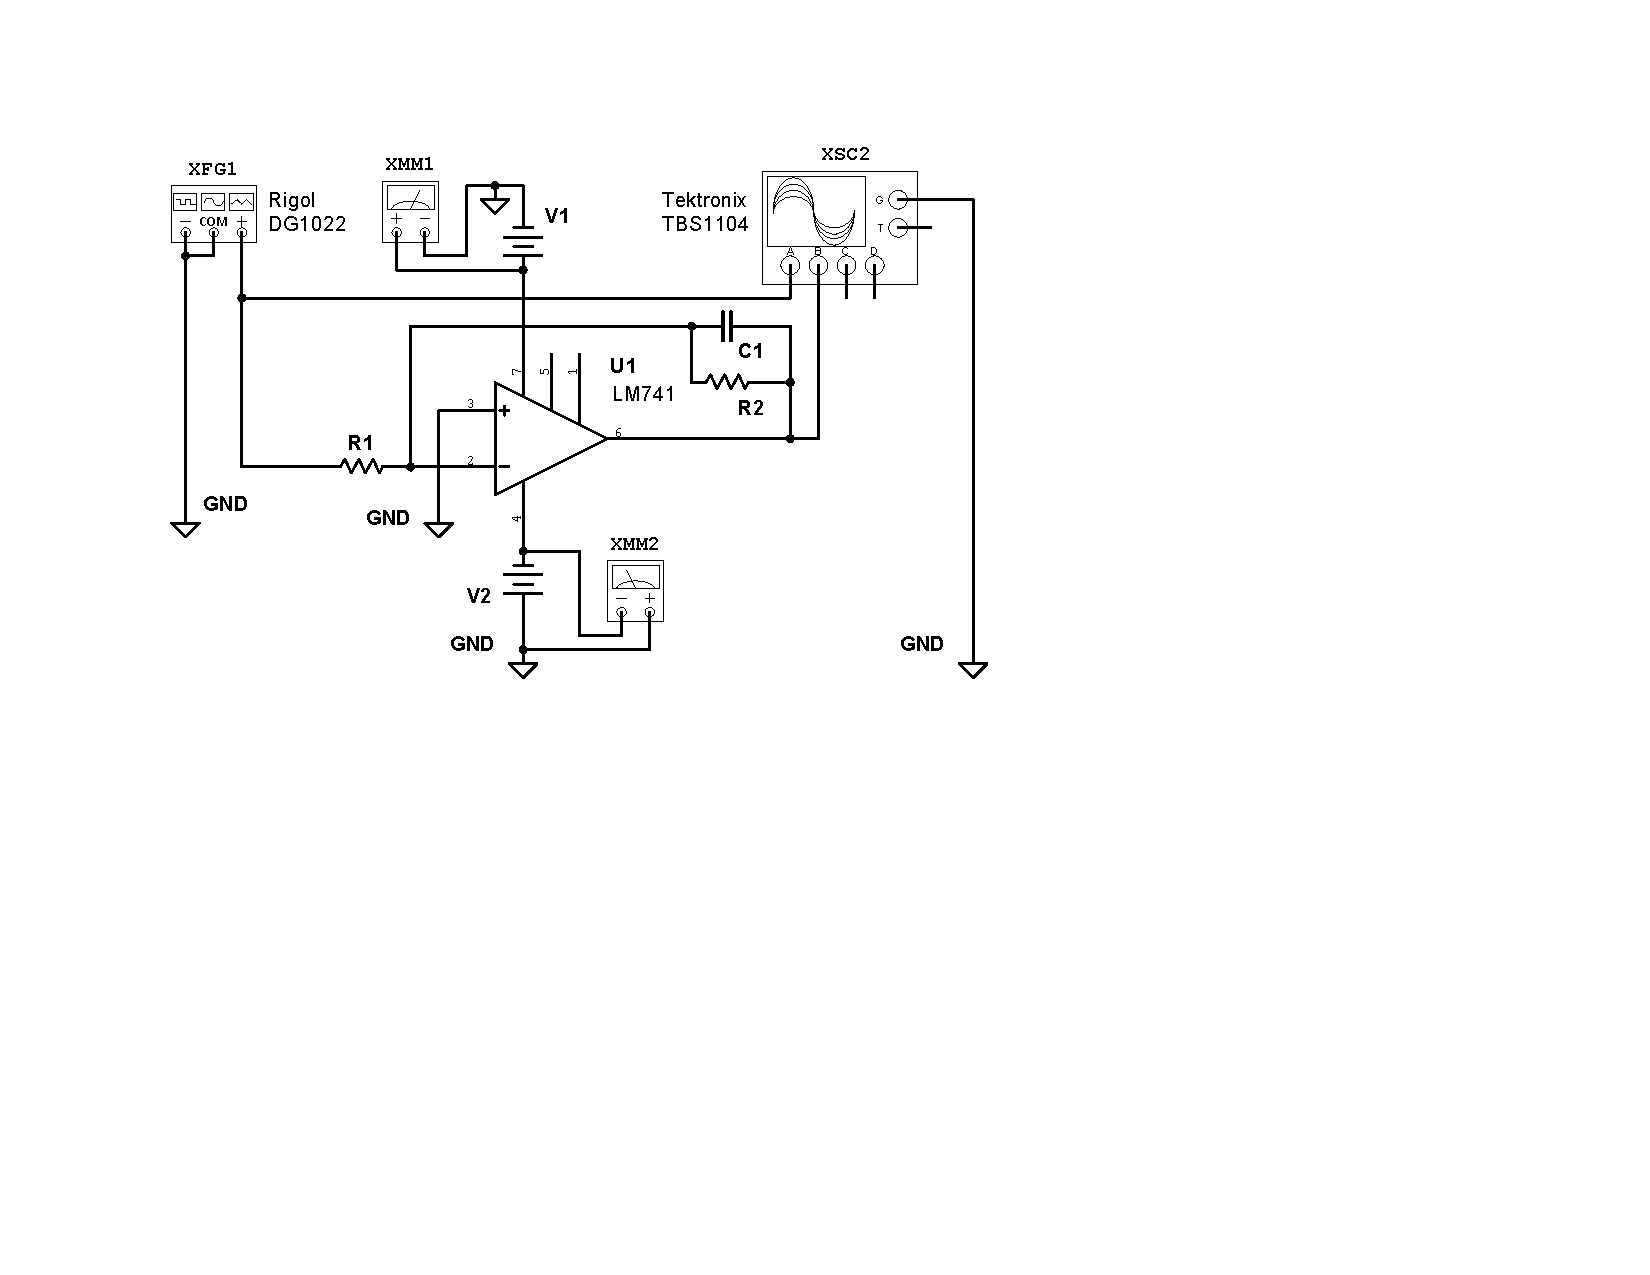
\includegraphics[width=0.38\textwidth]{sch-simulations/output/OPA-integratore.pdf}
\caption{Schema  del  circuito  elettrico  per  la  caratterizzazione  dell’OPA integratore.  Valori  per  i  componenti  utilizzati  misurati  con il multimetro: $R_1 = (9.9 \pm 0.1)\ k\Omega, \ R_2 = (9.9 \pm 0.1) \ k\Omega,\ C_1 = (23 \pm 1)\ nF$}
\label{fig:OPA-integ}
\end{center}
\end{figure}
%Come sottintende il nome, l'Op-Amp integratore è un operazionale che esegue l'operazione matematica dell'integrazione, facendo si che il circuito emetta una $V_{out}$ proporzionale all'integrale della $V_{in}$. In altre parole, facendo riferimento alla \ref{fig:OPA-integ}, l'ampiezza del segnale in uscita è determinato dal periodo di tempo in cui una tensione è presente in input, poiché la corrente attraverso il circuito di feedback carica o scarica il condensatore mentre il feedback negativo richiesto avviene attraverso il condensatore.
Mediante un amplificatore operazionale è possibile realizzare un circuito integratore, cioè in grado di produrre in uscita un segnale proporzionale alla primitiva della forma d'onda in ingresso, inserendo una capacità nella rete di feedback tra l'ingresso invertente e l'uscita.
Affinché l'amplificatore non vada in saturazione alle basse frequenze, viene aggiunto in parallelo a $C$ un resistore $R_{2}$ che fa si che in tale regime operativo il condensatore si comporti come una impedenza infinita, determinando un guadagno $A_{v}=-R_{2}/R{1}$. Questa configurazione è detta \textit{circuito integratore attivo limitato}. 
%essendo il periodo della tensione in ingresso relativamente lungo,
Una caratteristica importante è che il circuito si comporta effettivamente da integratore solo per frequenze superiori a quella di taglio, $f_{t}=\frac{1}{2 \pi C R_{1} }$, è quindi necessario scegliere $R$ e $C$ opportunamente, in relazione alla distribuzione spettrale del segnale da integrare. Questo è giustificabile osservando il grafico di fase del diagramma di Bode associato: oltre la frequenza di taglio tutte le armoniche sinusoidali di Fourier vengono sfasate di un angolo tale da essere approssimabili come inverse di cosinusoidi, cioè integrali delle sinusoidi di partenza.

\subsection{\textbf{Caratterizzazione}}
Inizialmente si sono scelte $R = (9.920 \pm 0.103) \ k\Omega \ e \ C = (23.4 \pm 1.2) \ nF$ con lo scopo di ottenere una frequenza di taglio non eccessivamente bassa per favorire lo studio della risposta in frequenza della fase successiva: \[f_{t} = \frac{1}{2 \pi R_{1} C}= 685.63 \pm 35.88 Hz\].

\begin{figure}[H]%[!ht]
\begin {center}
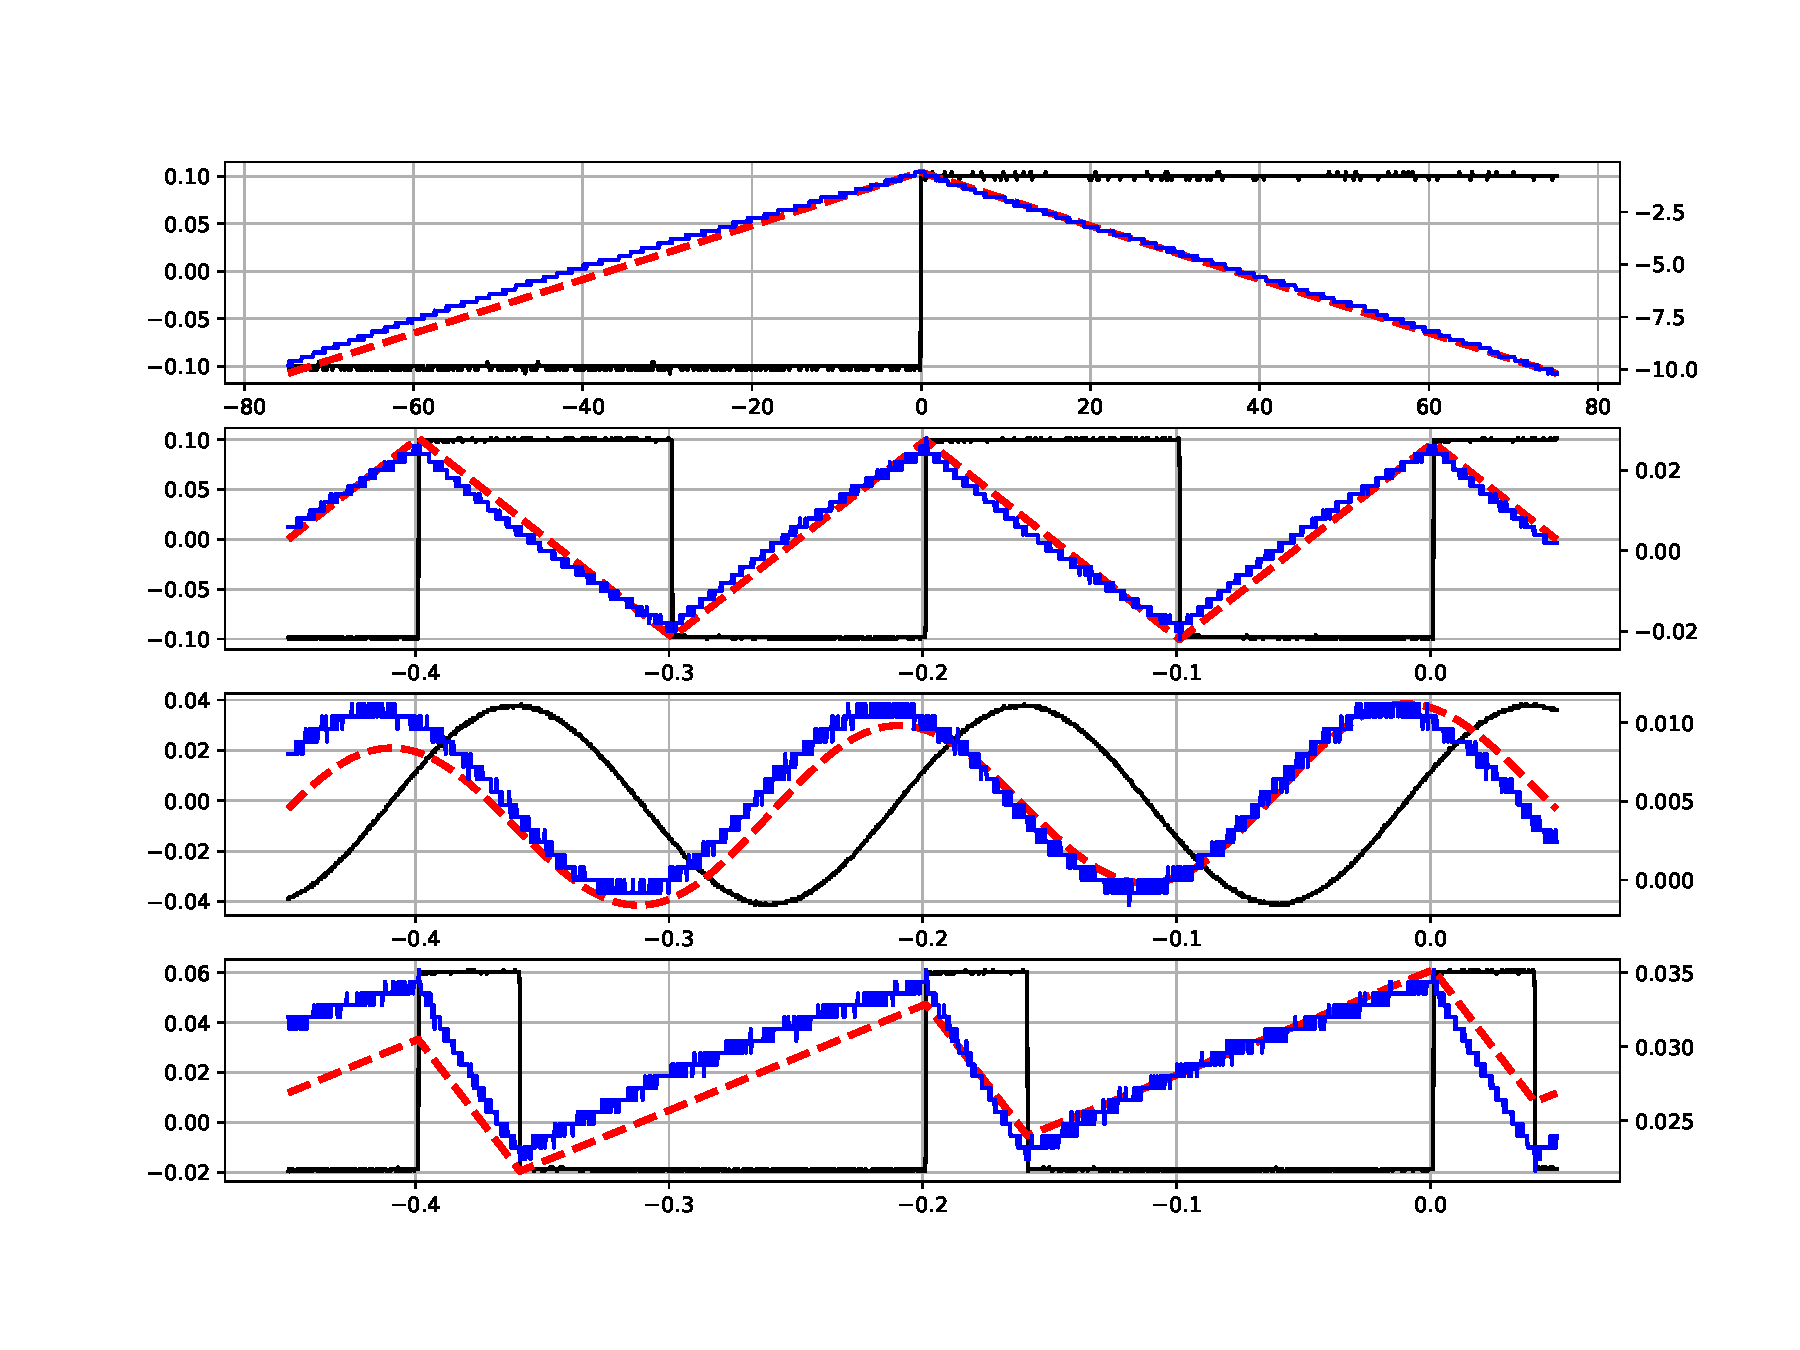
\includegraphics[width=0.50\textwidth]{analysis/output/OPA-integ-with-res.pdf}
\caption{Risposta del circuito integratore attivo a diverse forme d'onda in ingresso. Partendo dall'alto gradino, onda quadra, sinusoide e treno di impulsi}
\label{fig:OPA-integ-res}
\end {center}
\end{figure}
Impostando una frequenza, $f= 5 kHz$, si è proceduto con l'osservazione della risposta del circuito, \textit{Fig. \ref{fig:OPA-integ-res}}. Come atteso, la $V_{out}$ risulta essere molto vicina all'integrale del segnale in ingresso. In particolare si nota la compatibilità con l'integrale calcolato numericamente rappresentato dalla linea rossa tratteggiata, a meno di un termine lineare dovuto all'offset dell'integrando.

\subsection{\textbf{Studio della risposta in frequenza}}

Terminata la prima fase si è passati all'analisi dell'output del circuito in funzione della frequenza. I dati sono stati presentati su un grafico e interpolati in primo luogo con la forma funzionale di un filtro passa basso e poi in seguito con la funzione di trasferimento attesa, che risulta essere: 
\begin{equation}
    H(s) = -\frac{\frac{R_2}{R_1}}{1 + s(2 \pi C R_2)} = -\frac{\frac{R_2}{R_1}}{1 + \frac{s}{f_t}}
\end{equation}

con $f_H$ polo della funzione di trasferimento e $A_v(0)$ il valore di \textit{magnitude} alla frequenza nulla, estratto dalla regressione del fit. Il minimizzatore restituisce infatti per i parametri i seguenti valori:  f_H = (0.75 $\pm$ 0.01) kHz A_v(0) = (1.001 $\pm$ 0.003)
Dal confronto di $A_v(0)$ con il gain della $H(s)$ e tra $f_H$ ed $f_t$ si evince un'ottima compatibilità entro un livello di significatività del 5\% in entrambi i casi ($t_{Gain} = 0.39 $, $t_{Freq} = 1.45 $) .

\begin{figure}[H]%[!ht]
\begin{center}

\includegraphics[width=0.40\textwidth]{analysis/output/OPA-integrator_bode(mag+phase).pdf}
\caption{Diagramma di Bode del circuito integratore, nel quadrante superiore è illustrata l'ampiezza di tensione in scala dB, mentre nel quadrante inferiore la curva predetta per la fase dal modello utilizzato per interpolare i dati di ampiezza.}
\label{fig:integ-bode}
\end{center}
\end{figure}


%%%%%%%%%%%%%%%%%%%%%%%%%%%%%%%%%%%%%%%%%%
\subsection{\textbf{Considerazioni conclusive}}
Il circuito si dimostra conforme a quanto atteso, infatti i segnali di output risultano approssimare correttamente gli integrali numerici delle forme d'onda in ingresso quando la frequenza del segnale integrando è sufficientemente elevata, confrontata con la frequenza di taglio. E' importante sottolineare il fatto che il circuito integratore tenda a ridurre il rumore del segnale in ingresso, come si evince della \textit{Fig. \ref{fig:OPA-integ-res}}, comportamento opposto a quello di un OPA derivatore. Si vuole inoltre sottolineare, in riferimento alla figura \ref{fig:integ-bode}, che volendo caratterizzare correttamente la risposta in frequenza anche per attenuazioni elevate, alcuni punti ad alta frequenza hanno un errore relativo che in scala logaritmica risulta particolarmente elevato. Questo è dovuto ai limiti della risoluzione verticale dell'oscilloscopio.

%%%%%%%%%%%%%%%%%%%%%%%%%%%%%%%%%%%%%%%%%%
\section{\textbf{Amplificatore derivatore}} %Matteo
\subsection{\textbf{Circuito}}
\begin{figure}[H]%[!ht]
\begin{center}
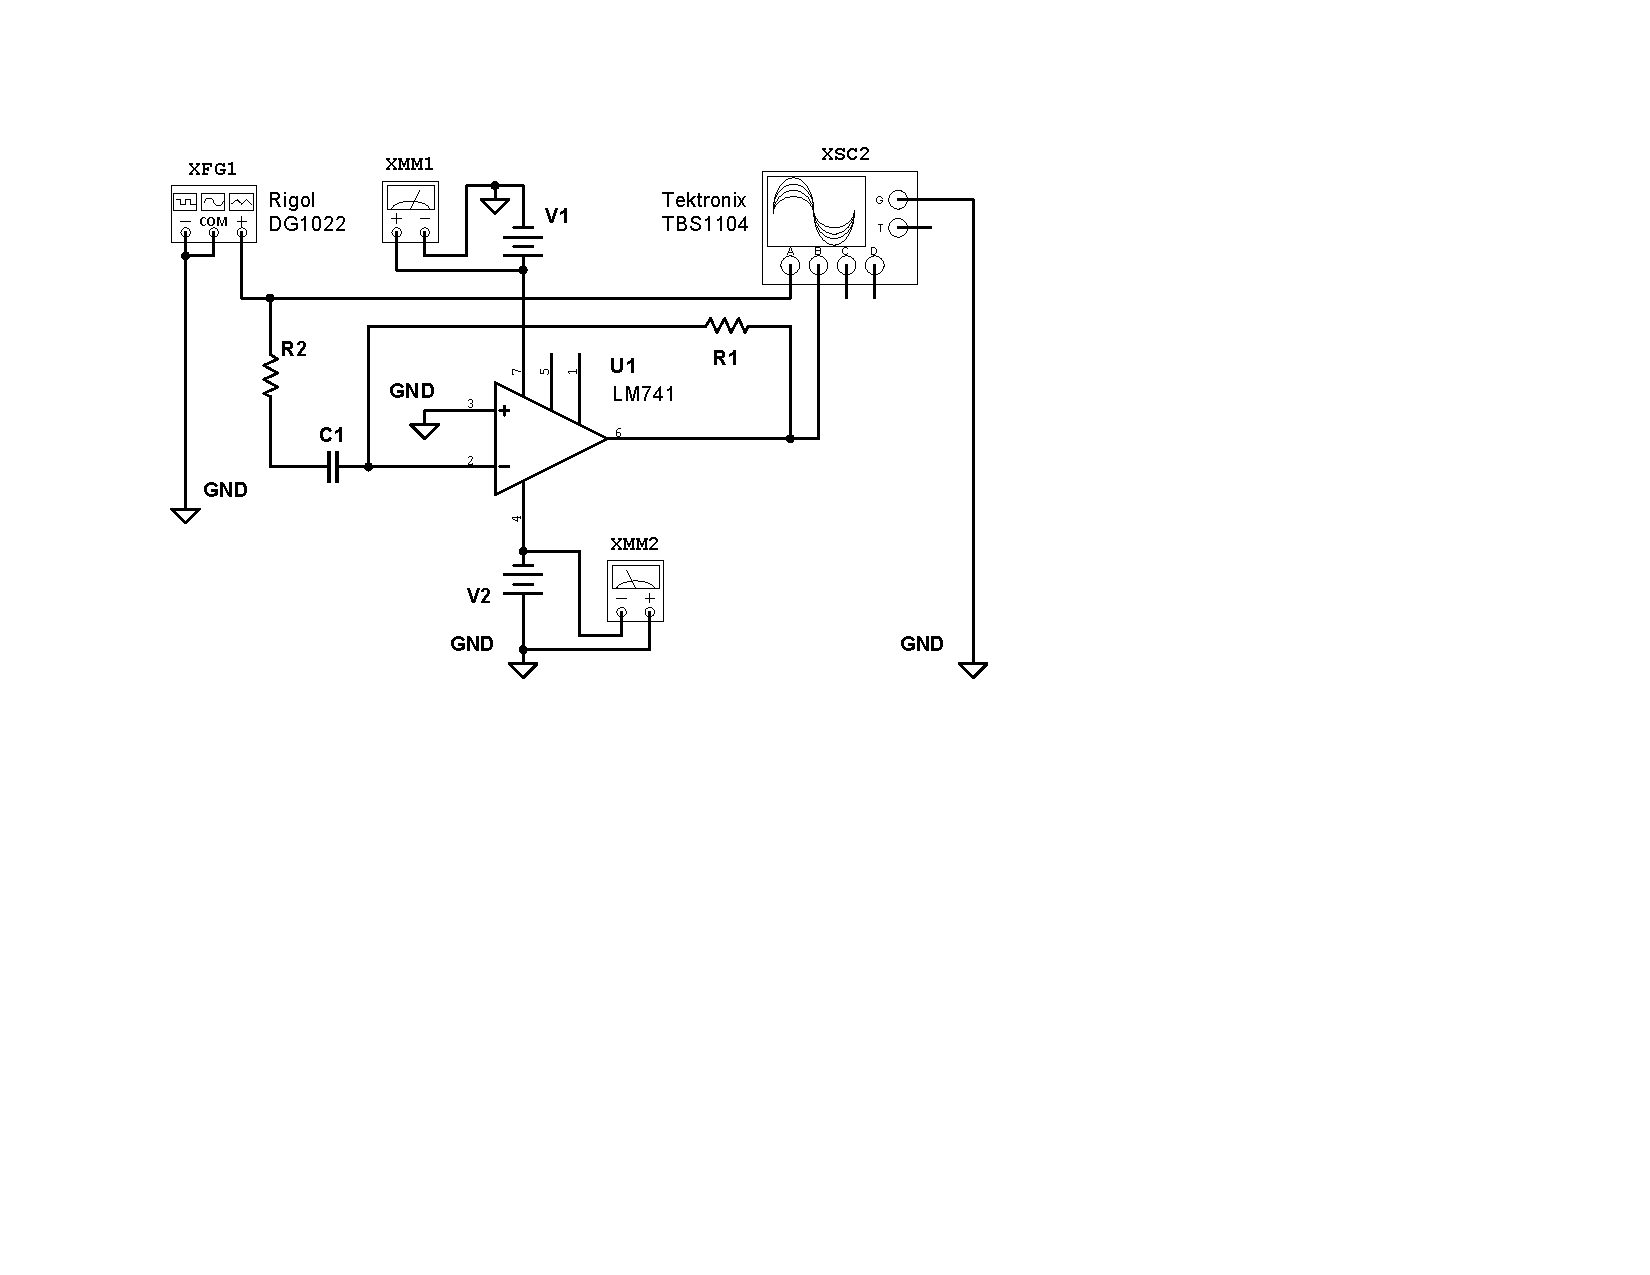
\includegraphics[width=0.38\textwidth]{sch-simulations/output/OPA-deriv.pdf}
\caption{Schema  del  circuito  elettrico  per  la  caratterizzazione  dell’OPA derivatore.  Valori  per  i  componenti  utilizzati  misurati  con  il  multimetro: R1= $(9.920 \pm 0.103)$ $k\Omega$, R2= $(9.850 \pm 0.102)$ $k\Omega$, C1= $(23.4 \pm 1.2)$ $\ nF$}
\label{fig:OPA-deriv}
\end{center}
\end{figure}

Rispetto al circuito integratore presentato sopra, nel caso del circuito derivatore le posizioni del condensatore e del resistore sono state invertite affinché il condensatore $C$ sia collegato al terminale di ingresso dell'amplificatore invertente mentre il resistore $R_1$ costituisca l'elemento di feedback negativo. Questo circuito esegue l'operazione matematica di differenziazione, cioè produce un'uscita di tensione proporzionale alla velocità di variazione della tensione di ingresso e alla corrente che scorre attraverso il condensatore. Si noti che il condensatore blocca qualsiasi contenuto \textit{DC} della tensione in ingresso, consentendo  quindi il solo passaggio di segnali di tipo \textit{AC}. Alle basse frequenze la reattanza del condensatore è elevata con conseguente guadagno basso ($\frac{R_1}{X_C}$) e bassa tensione di uscita, mentre per alte frequenze si avrà un guadagno nettamente maggiore, si è infatti realizzato un filtro passa alto attivo. 
%E' possibile ridurre il guadagno ad alta frequenza introducendo utililizzando un resistore di feedback $R_f$ di resistenza ridotta. 

\subsection{\textbf{Valutazione della risposta a differenti forme d'onda in ingresso}}
Una volta assemblato il circuito si è proseguito analizzando qualitativamente il comportamento a segnali in input di diversa forma d'onda, verificando che l'output fosse in accordo con quello previsto.

\begin{figure}[H]%[!ht]
\begin{center}
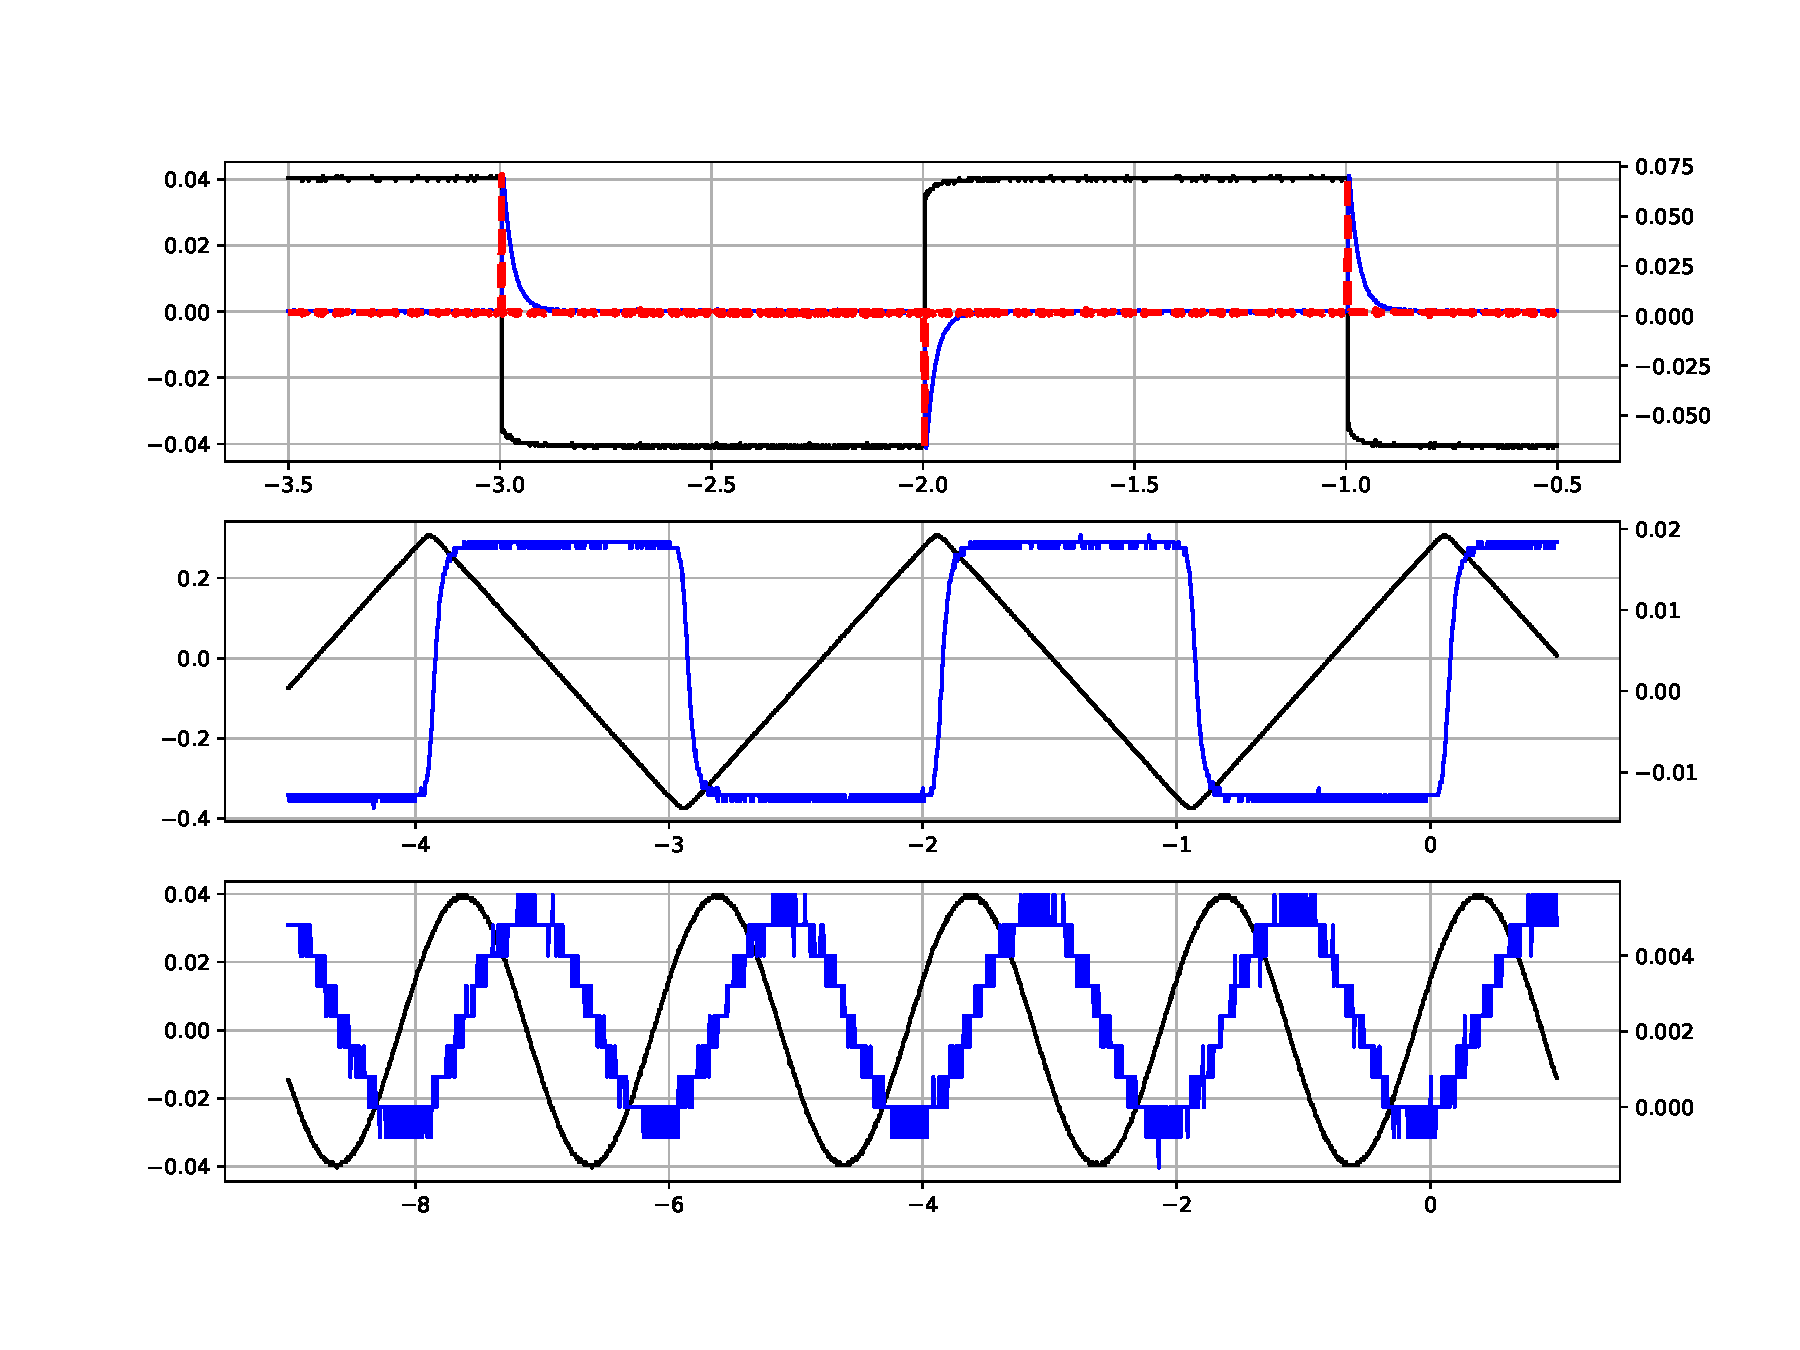
\includegraphics[width=0.50\textwidth]{analysis/output/OPA-differentiator.pdf}
\caption{Risposta del circuito derivatore reale a diverse forme d’onda in ingresso. Partendo dall’alto gradino, onda quadra, onda a dente di sega e sinusoide. La derivata dell'onda quadra sarebbe teoricamente una delta di Dirac, che però non può esistere a livello sperimentale perché richiederebbe banda infinita.}
\label{fig:derivatore}
\end{center}
\end{figure}

Dalla \textit{Fig. \ref{fig:derivatore}}, in cui le scale dei voltaggi sono diverse fra input e output col fine di ottimizzarne la comprensibilità visiva, si vede come il segnale in uscita sia effettivamente paragonabile con la derivata della $V_{in}$. In particolare valutando lo sfasamento tra le due forme d'onda si trova $\theta = 87.23 \deg$, compatibile con 90 deg, che corrisponde ad un'integrazione termine a termine di tutte le componenti di Fourier del segnale in ingresso.

Il funzionamento osservato è quindi in accordo con le previsioni teoriche. Ovviamente è necessario tener conto del fatto che la bontà della derivazione dipende, come ampiamente discusso nel caso dell'integratore, strettamente dalla frequenza del segnale in ingresso. Infatti se quest'ultima non fosse stata molto minore rispetto alla frequenza di taglio il circuito avrebbe agito da semplice amplificatore invertente, dal momento che avrebbe introdotto uno sfasamento trascurabile alle componenti sinusoidali di Fourier.

%%%%%%%%%%FINE SECONDO GIORNO%%%%%%%%%%%%%%%
%%%%%%%%%%INIZIO TERZO GIORNO%%%%%%%%%%%%%%%

%%%%%%%%%%%%%%%%%%%%%%%%%%%%%%%%%%%%%%%%%%
\section{\textbf{Mixer invertente}} %Federico
Sulla \textit{breadboard} è stato implementato il circuito in \textit{Fig. \ref{fig:OPA-mixer}}. In questa configurazione, l'amplificatore si comporta come circuito sommatore ed il segnale in uscita sarà proporzionale alla somma dei segnali in ingresso. L'OPA è collegato in configurazione invertente, dunque in uscita si otterrà la somma dei segnali cambiata di segno. Nello specifico: 

\begin{equation}
V_{out} = - R  \sum_{n} \frac{V_n}{R_n} = - \sum_{n} V_n 
\end{equation}

Il circuito mixer realizzato in laboratorio non aggiunge amplificazione ai segnali, questo si ottiene scegliendo tutti i valori delle resistenze circa uguali ($R = R_1 = R_2$). Nel nostro caso si ha: $R_1 =(9.81 \pm 0.13) \ k\Omega, \ R_2 = (9.95 \pm 0.13) \ k\Omega ,\ R_3 = (9.89 \pm 0.13) \ k\Omega$.

I primi due canali dell'oscilloscopio sono collegati ai segnali $V_1$ e $V_2$ prodotti dal generatore di funzioni, mentre il terzo canale misura la tensione in uscita $V_{out}$.


\begin{figure}[H]%[!ht]
\begin{center}
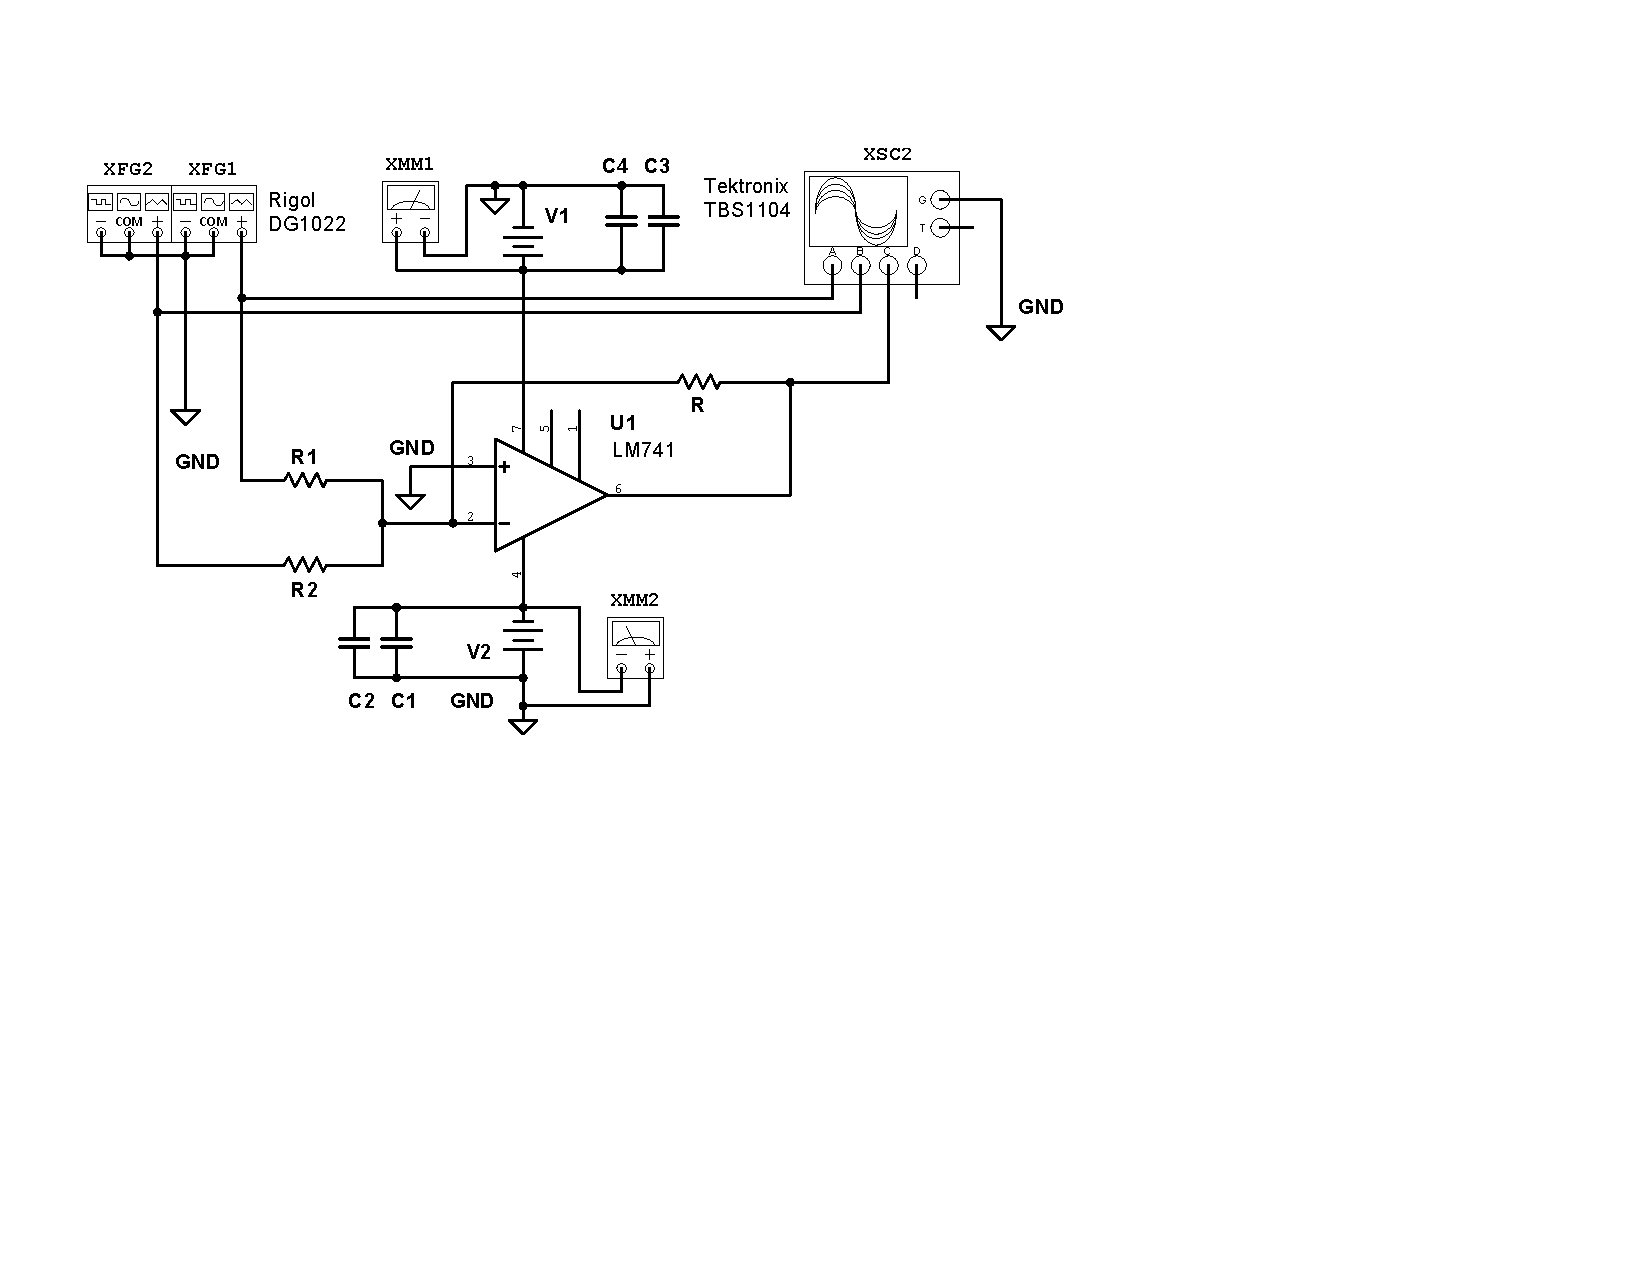
\includegraphics[width=0.45\textwidth]{sch-simulations/output/OPA-mixer.pdf}
\caption{Schema  del  circuito  elettrico  per  la  caratterizzazione  della configurazione invertente del circuito sommatore. Valori per i componenti utilizzati misurati con il multimetro: R1= $(9.81 \pm 0.101)$ $k\Omega$, R2= $(9.95 \pm 0.104)$ $k\Omega$, R3= $(9.89 \pm 0.103)$ $k\Omega$}
\label{fig:OPA-mixer}
\end {center}
\end{figure}

\vspace{-10mm}


\subsection{\textbf{Somma di forme d'onda sinusoidali}}
In un primo momento agli ingressi dell'amplificatore sono state mandate due sinusoidi in fase con ampiezza $V_1 = V_2 = 0.5 V$. La somma dei due segnali risulta essere una nuova sinusoide di ampiezza $V_{out} = 1 V$ con segno opposto a quelle in ingresso (come da \textit{fig. \ref{fig:Mixer1}})
Lo stesso effetto si ha per sinusoidi con ampiezze diverse ($V_1 = 0.5, V_2 = 0.25 V$) in \textit{figura \ref{fig:Mixer3} }. La tensione in uscita risulta effettivamente avere ampiezza pari alla somma delle ampiezze delle onde in ingresso.

\begin{figure}[H]%[!ht]
\begin{center}
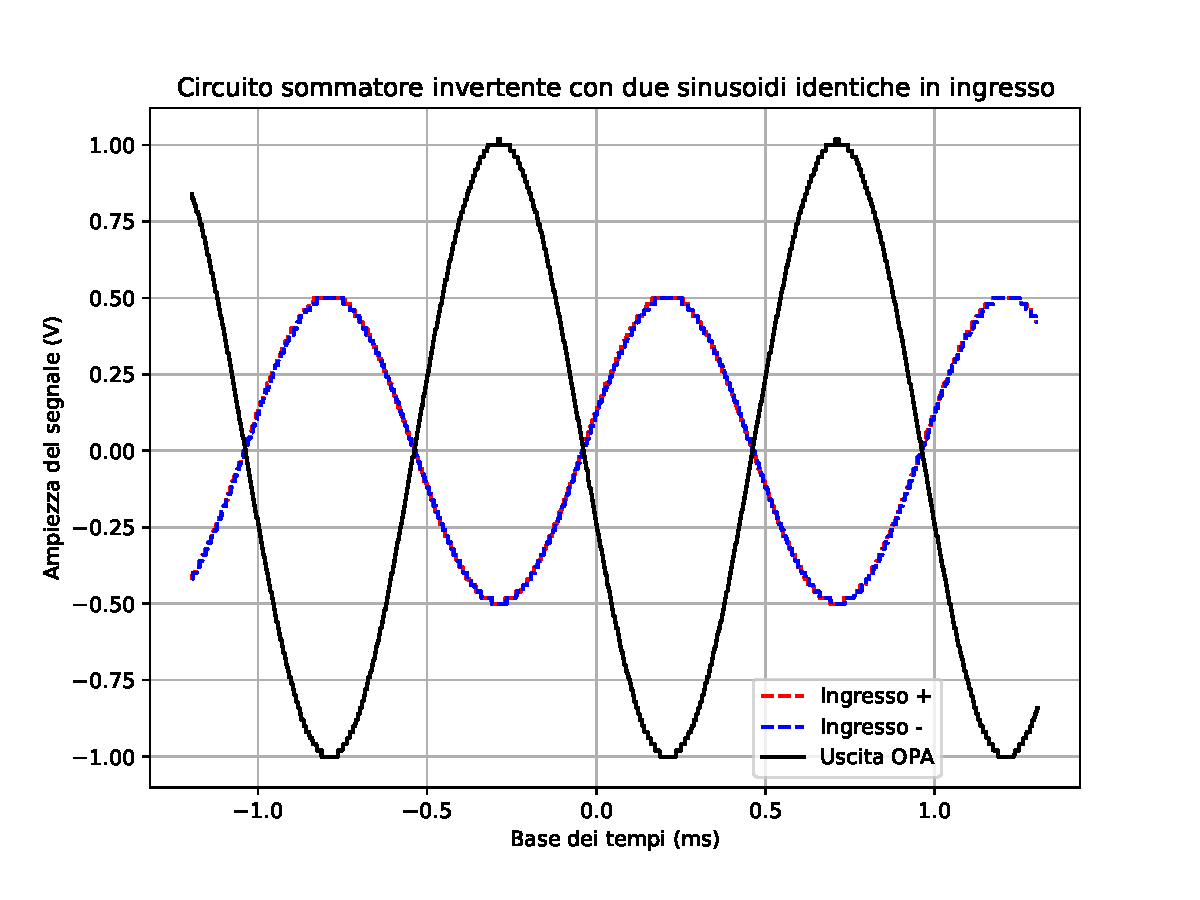
\includegraphics[width=0.46\textwidth]{analysis/output/OPA_mixer_sin0.pdf}
\caption{Somma di sinusoidi identiche}
\label{fig:Mixer1}
\end{center}
\end{figure}

\begin{figure}[H]%[!ht]
\begin{center}
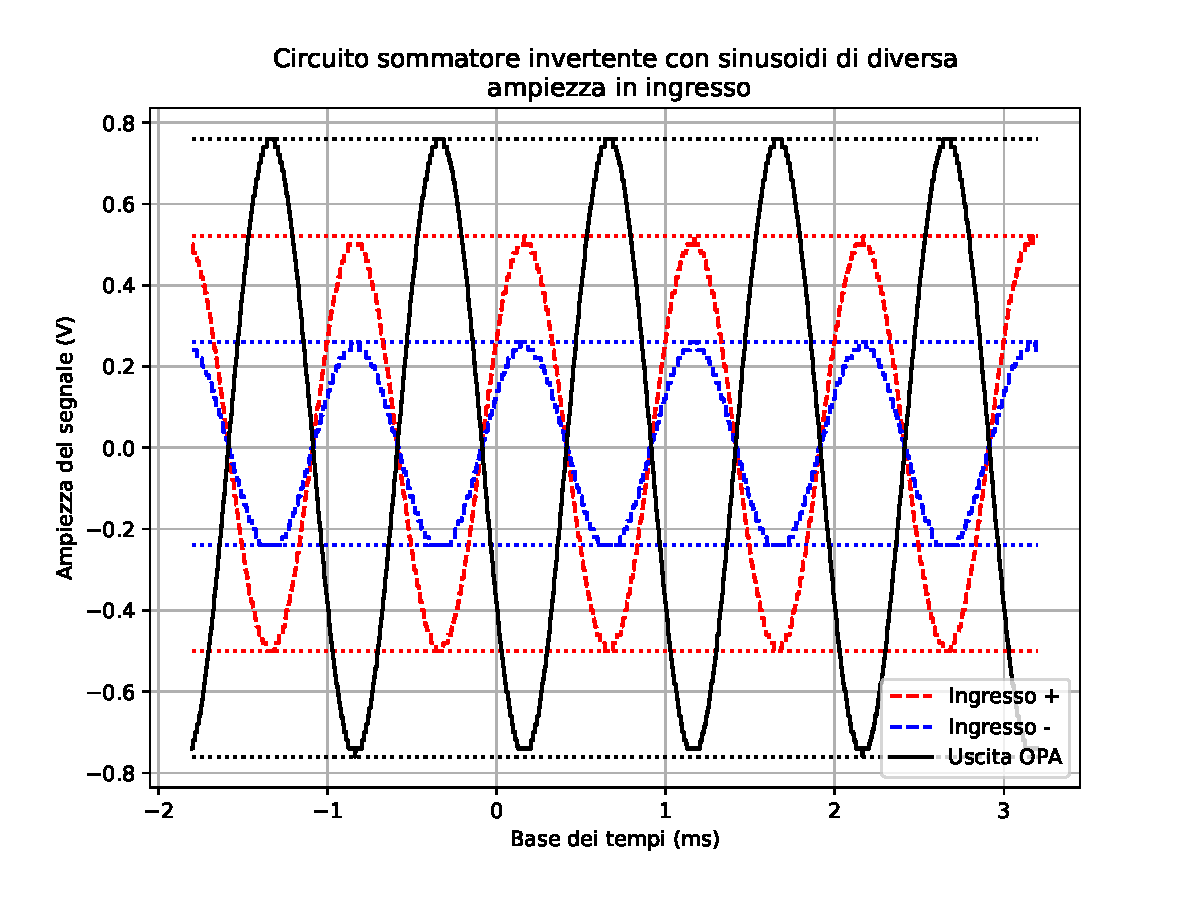
\includegraphics[width=0.46\textwidth]{analysis/output/OPA_mixer_sin3.pdf}
\caption{Somma di sinusoidi in fase con mixer non invertente}
\label{fig:Mixer3}
\end{center}
\end{figure}

\begin{figure}[H]%[!ht]
\begin{center}
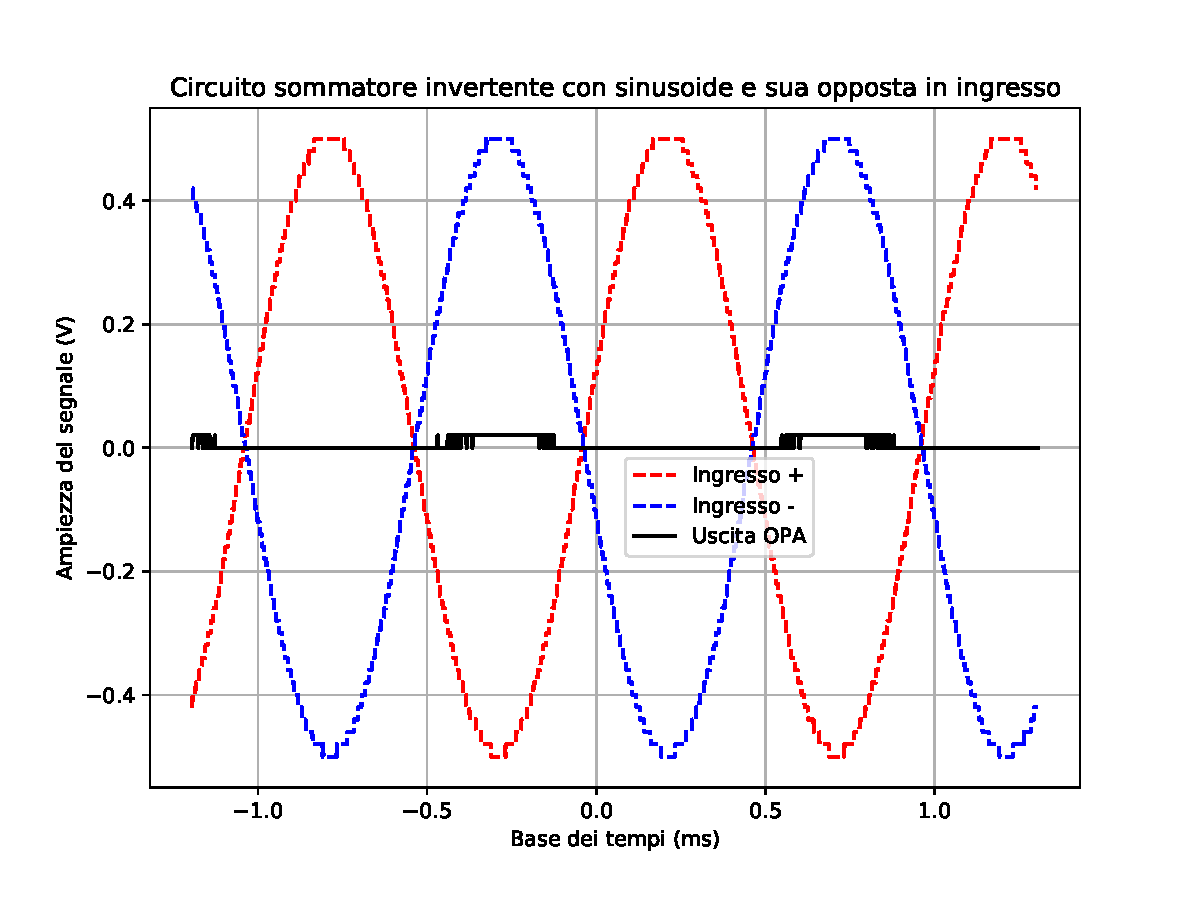
\includegraphics[width=0.46\textwidth]{analysis/output/OPA_mixer_sin2.pdf}
\caption{Somma di una funzione sinusoidale con la sua opposta}
\label{fig:Mixer2}
\end{center}
\end{figure}

Sostituendo il segnale all'ingresso negativo con la sinusoide opposta, si ottiene all'uscita un segnale sostanzialmente nullo, frutto dalla somma di forme d'onda opposte di uguale ampiezza come evidenziato in \texit{fig. \ref{fig:Mixer2}}. Il leggero distaccamento dallo zero del segnale in uscita è causato dal fatto che $R_1$ e $R_2$ non sono esattamente identiche, dunque la formula (1) non è una somma diretta ma è pesata sui valori delle resistenze collegate. Questa configurazione coincide con quella dell'amplificatore di differenze di segnali quando in ingresso riceve due sinusoidi identiche. (Vedi paragrafo \ref{par:differenze})

 Si è infine svolta una verifica qualitativa della linearità dell'amplificazione del canale non invertente effettuando una regressione lineare sullo scatter dei dati estratti in visualizzazione $X-Y$ mettendo a confronto $Ch_1$ con l'uscita.
\begin{figure}[H]%[!ht]
\begin{center}
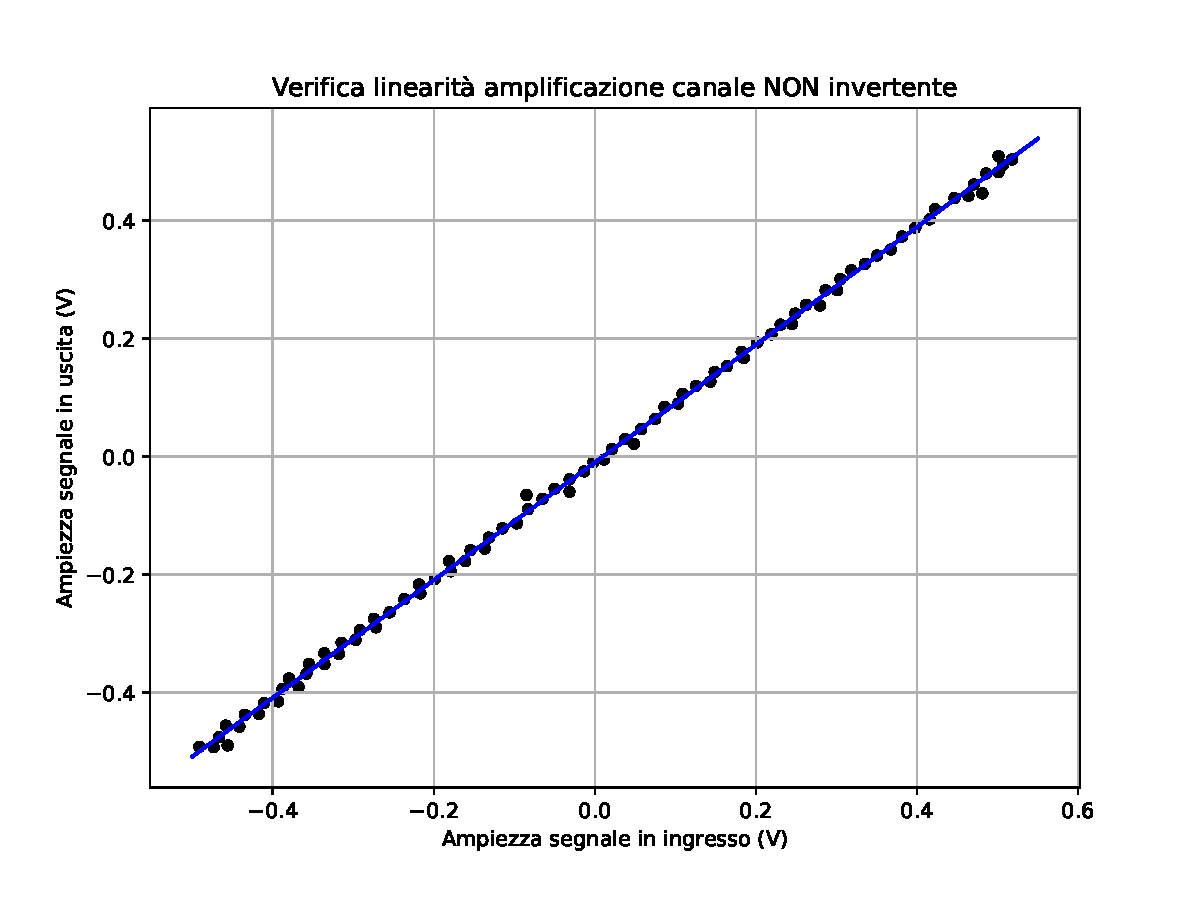
\includegraphics[width=0.50\textwidth]{analysis/output/OPA-linfit-non-inv.pdf}
\caption{Regressione lineare ($y$ = $ax$ +$b$) del canale non invertente in modalità $X-Y$ dell'oscilloscopio ($Ch_{in}-Ch_{out}$)}
\label{fig:lin-non-inv}
\end{center}
\end{figure}
Il minimizzatore di $\chi^2$ restituisce p-value del test di adattamento $\sim$ 1 e i seguenti valori per i parametri di fit
\[a = 0.997 \pm 0.003 \]
\[b = (-0.0097 \pm 0.0009) V \]
Effettuando un test di compatibilità tra il coefficiente angolare $a$ ed il suo valore atteso $a_e = 1$ si può affermare che i due dati  siano effettivamente compatibili con un livello di significatività superiore al 5\%, infatti $Z=0.99$.

\subsection{\textbf{Formazione di battimenti}}
Mandando ai due ingressi sinusoidi con frequenza leggermente diversa $f_1 $\sim$ 1.0\ kHz, \ f_2 $\sim$ 1.1\ kHz$ e uguale ampiezza (1 V), con $\Delta f$ >> f, si può avere la generazione di battimenti. Si osserverà quindi nella forma d'onda in uscita un inviluppo sinusoidale con frequenza f' $\sim$ 100 Hz. Si veda la \textit{figura \ref{fig:beats}}.

\begin{figure}[H]%[!ht]
\begin{center}
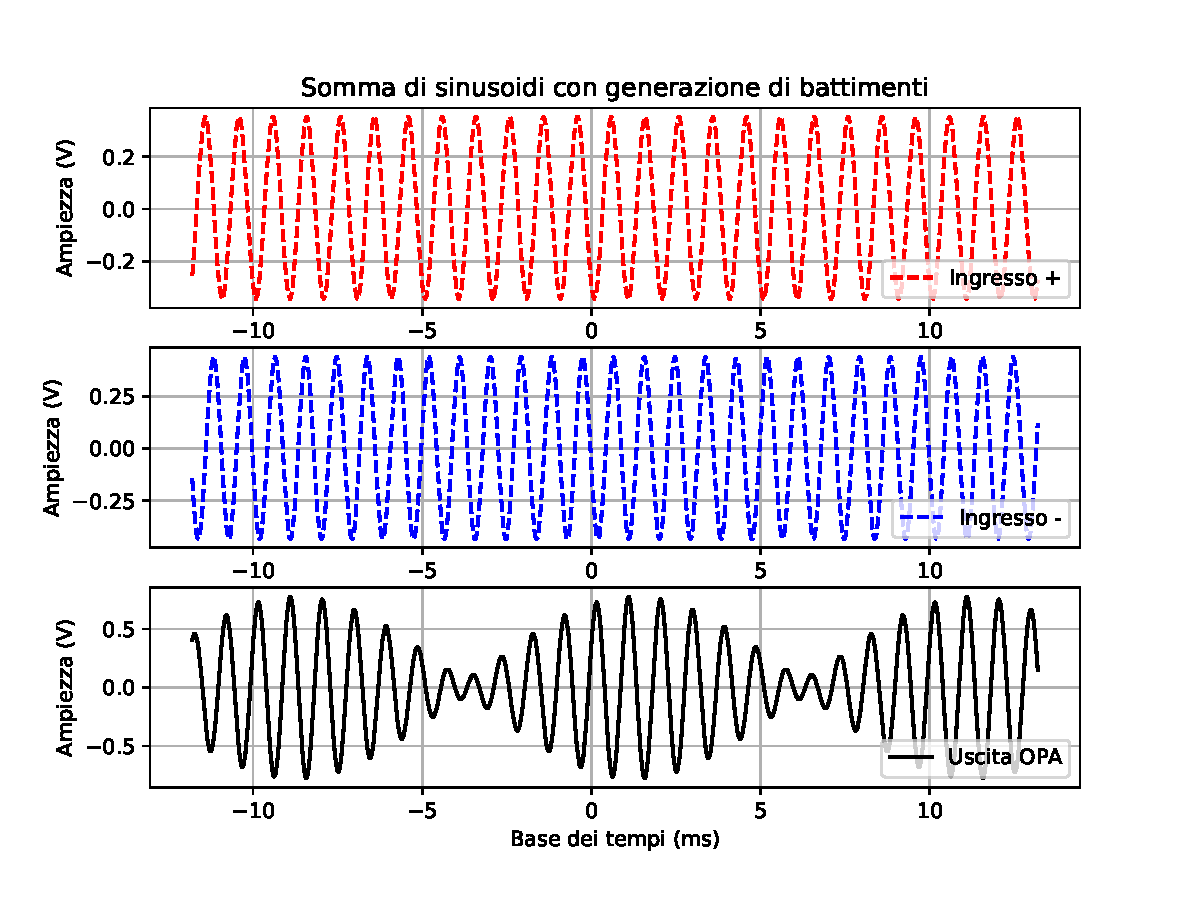
\includegraphics[width=0.42\textwidth]{analysis/output/OPA_mixer_beats.pdf}
\caption{Somma di sinusoidi identiche, ma con frequenze che differiscono di una quantità $\Delta f$ = 10 Hz, con $f_2 = f_1 + \Delta_f$ e $f_1$ = Hz  danno origine a battimenti di frequenza $f_b$ = Hz}
\label{fig:beats}
\end{center}
\end{figure}


%%%%%%%%%%%%%%%%%%%%%%%%%%%%%%%%%%%%%%%%%%
\section{\textbf{Amplificatore di differenze invertente \label{par:differenze}}} %Federico
\subsection{\textbf{Introduzione}}
Mediante un amplificatore operazionale è possibile realizzare un amplificatore di differenze inviando a ciascun ingresso dell'OPA un operando mediante opportune resistenze di ingresso e rete di feedback resistiva per controllare il guadagno. In laboratorio è stato implementato il circuito in \textit{figura \ref{fig:differenze}}, per il quale vale la seguente relazione: 
\begin{equation}
    V_{out} =\frac{V_2 - V_1}{K} \quad con \quad K = \frac{R_1}{R_2}=\frac{R_3}{R_4} \tag{2}
\end{equation}
Scegliendo le resistenze con valori identici ($R_1 = R_2 = R_3 =R_4 $) si otterrà quindi la differenza senza amplificazione dei segnali all'uscita dell'amplificatore cambiata di segno, poiché l'amplificatore è collegato in configurazione invertente.

\begin{figure}[H]%[!ht]
\begin {center}
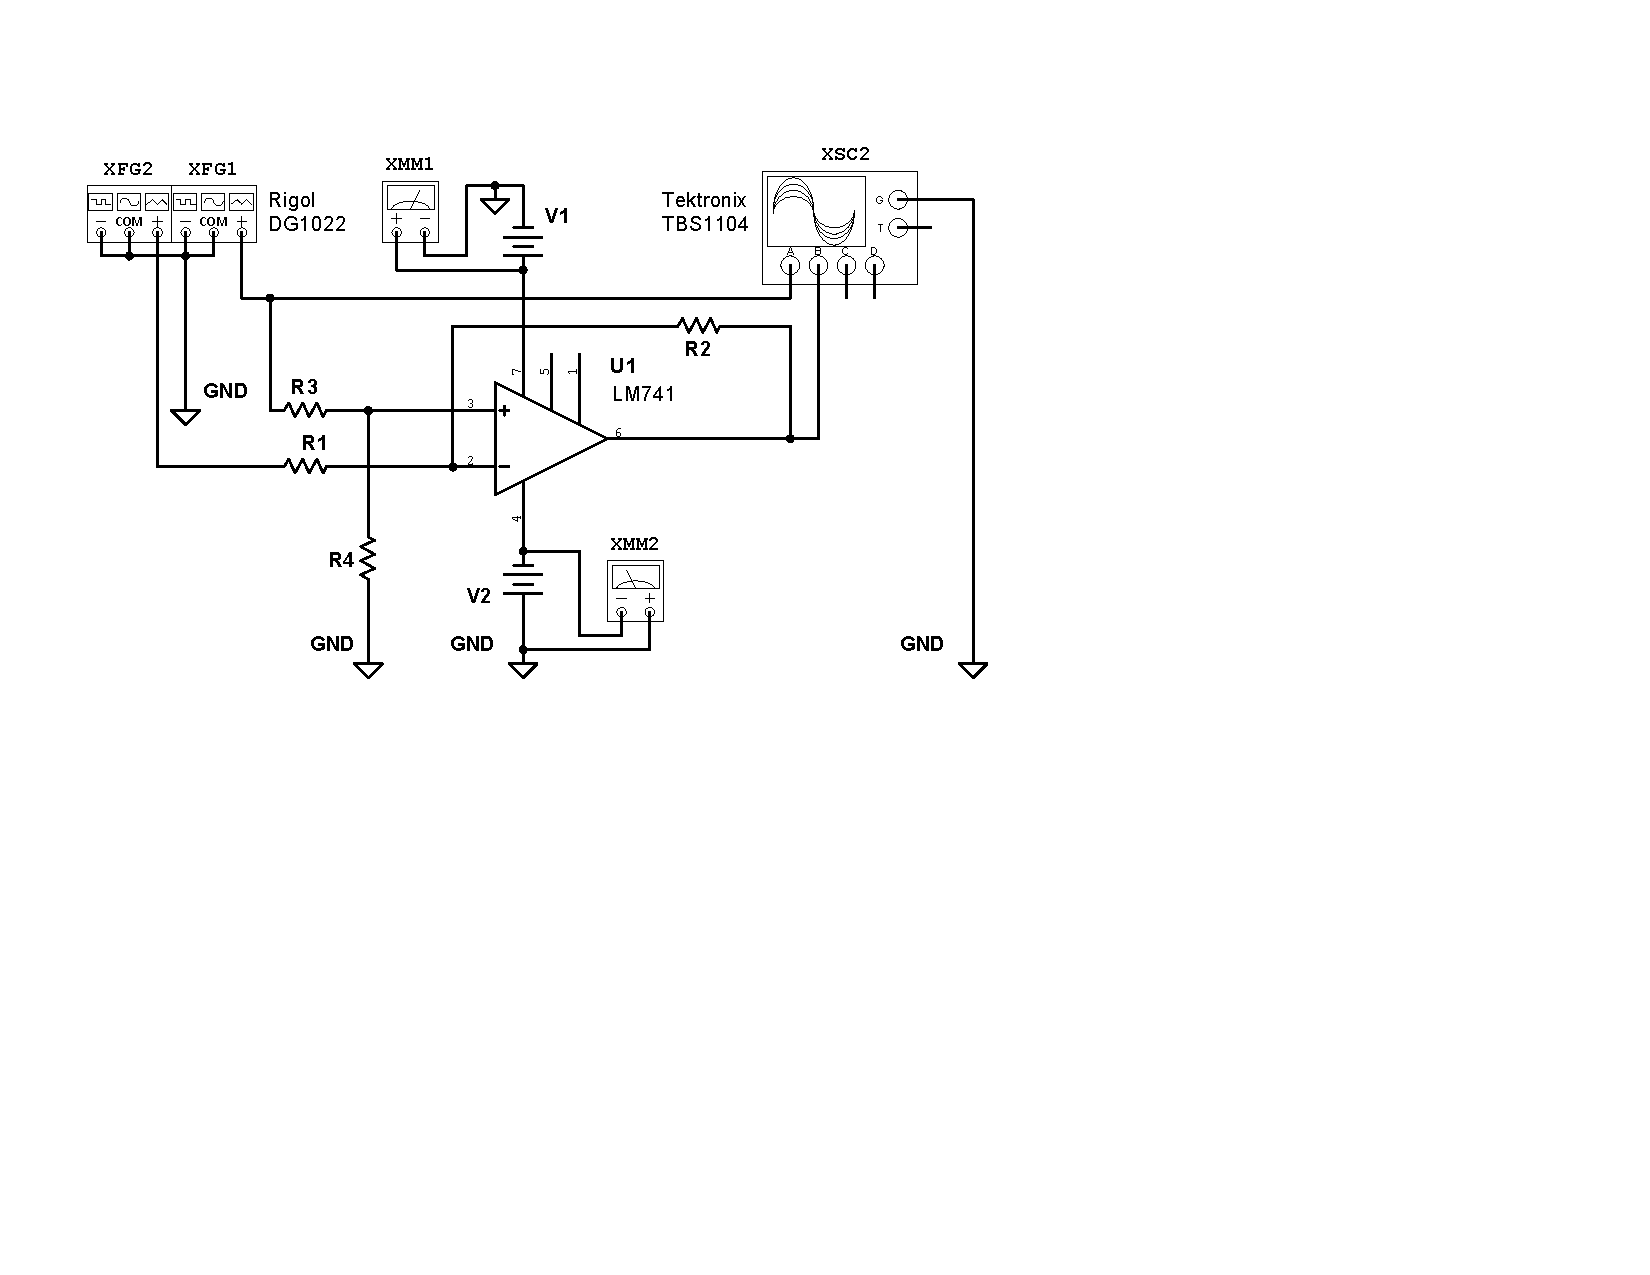
\includegraphics[width=0.38\textwidth]{sch-simulations/output/OPA-difference-amp.pdf}
\caption{Circuito amplificatore di differenze invertente. Sono stati usati i seguenti valori di resistenze: $R_1 =(9.81 \pm 0.13) \ k\Omega, \ R_2 = (9.95 \pm 0.13) \ k\Omega ,\ R_3 = (9.89 \pm 0.13) \ k\Omega \ e \ R_4 = (9.83 \pm 0.13) k\Omega  $  }
\label{fig:differenze}
\end {center}
\end{figure}

\subsection{\textbf{Differenze di onde sinusoidali}}
Per verificare il corretto funzionamento di questa configurazione sono state mandate agli ingressi due sinusoidi identiche in fase (ampiezza $0.5 V$). 

\begin{figure}[H]%[!ht]
\begin {center}
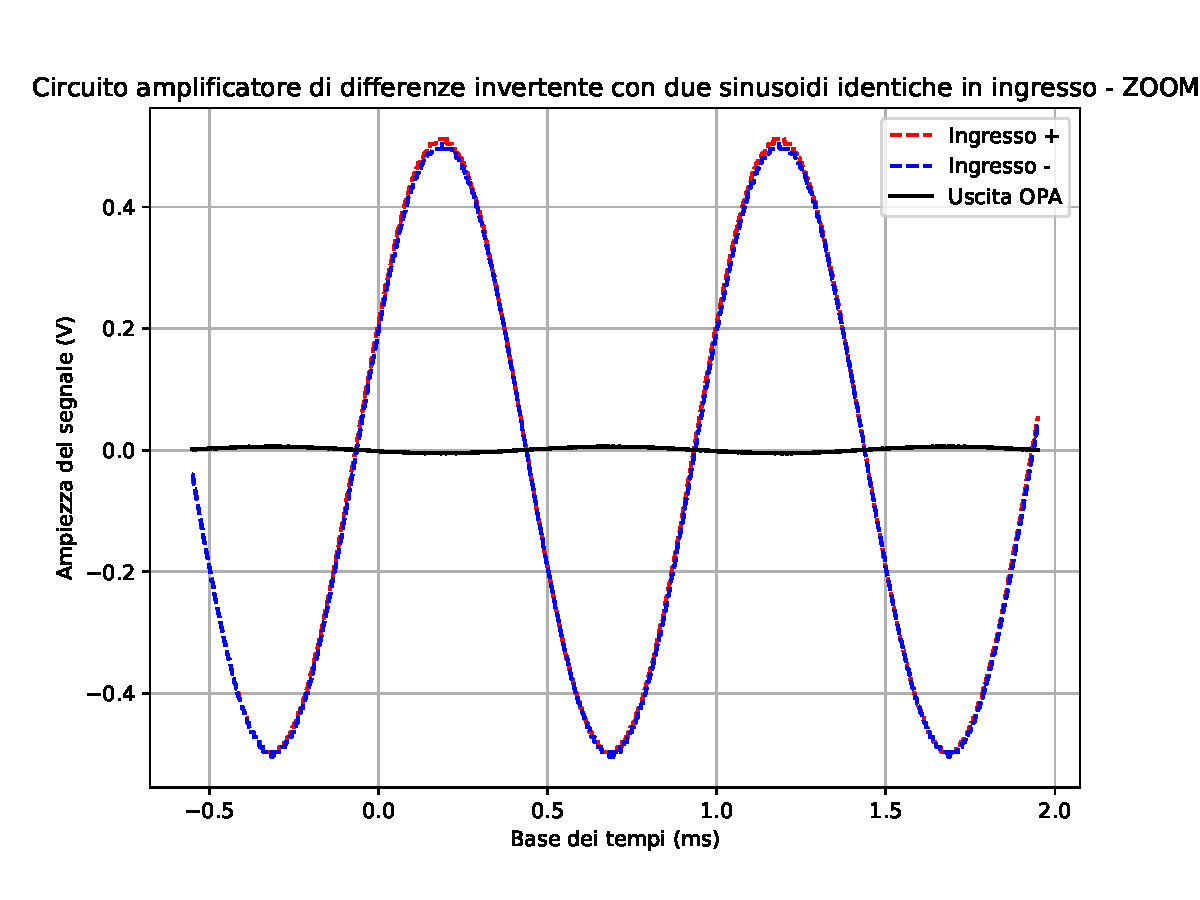
\includegraphics[width=0.50\textwidth]{analysis/output/OPA_diff_sin2.pdf}
\caption{Sottrazione di sinusoidi identiche}
\label{fig:diff2}
\end {center}
\end{figure}

Il grafico mostra che in uscita si registra una tensione praticamente nulla. Come nel sommatore, il lieve distacco dallo zero è da imputare alle piccole differenze del valore delle resistenze di ingresso.

Si è poi applicata una sinusoide a media nulla al primo canale e una sinusoide a media $-0.2 V$ al secondo, con ampiezza uguale alla prima, all'uscita si può visualizzare un segnale DC pari all'offset in tensione \textit{(Si veda la figura \ref{fig:diff3})}. 

\begin{figure}[H]%[!ht]
\begin {center}
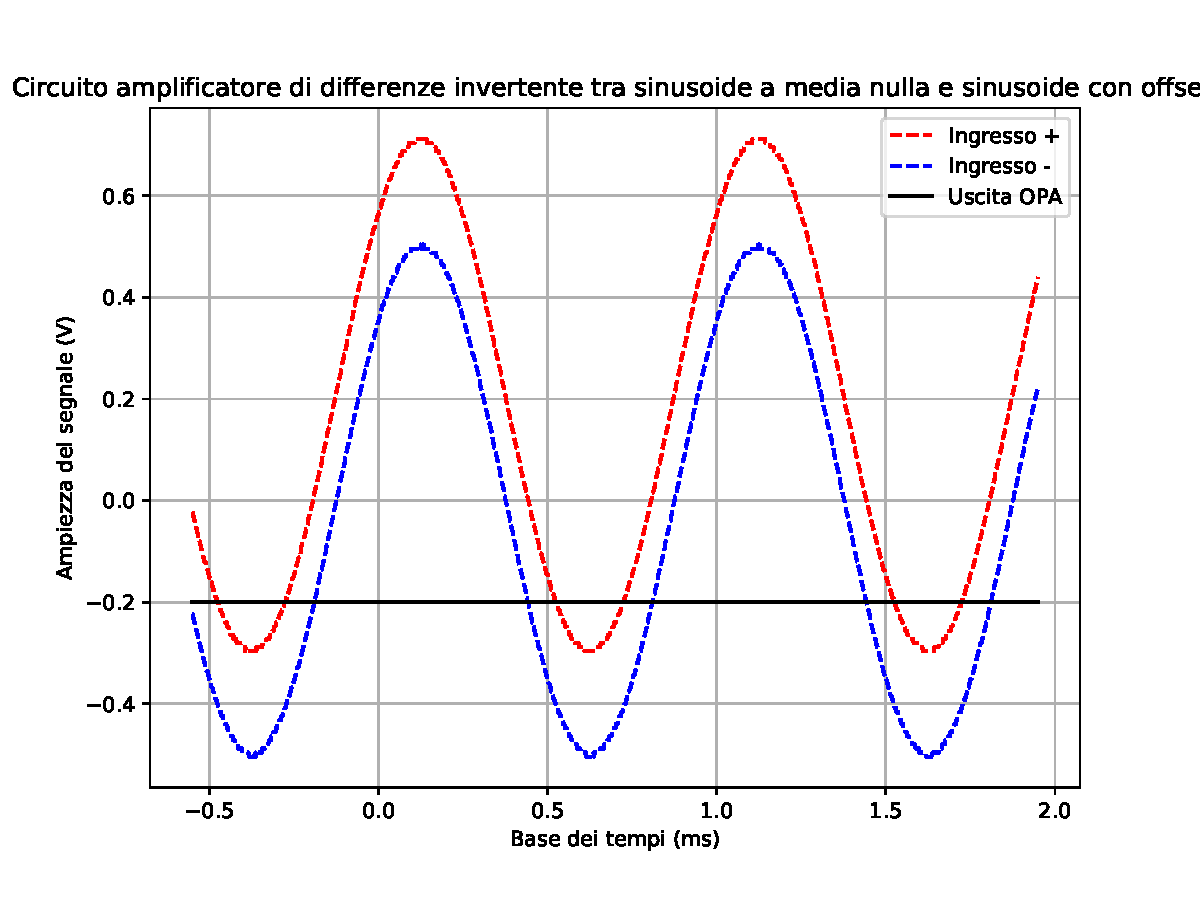
\includegraphics[width=0.50\textwidth]{analysis/output/OPA_diff_sin3.pdf}
\caption{Sottrazione da una funzione sinusoidale con offset di una componente DC di ampiezza pari all'offset, con risultato pari ad una sinusoide con media nulla}
\label{fig:diff3}
\end {center}
\end{figure}

\subsection{\textbf{Differenza di ulteriori forme d'onda e verifica della linearità}}
Nei grafici che seguono è possibile visualizzare la differenza di onde quadre con ampiezze diverse ($V_{+_max} = 0.5V \quad e \quad V_{-_max} = 0.25V$) in \textit{fig. \ref{fig:diff_square}}
e la differenza tra un'onda quadra e una rampa entrambe di ampiezza massima $V=0.5V$ in \textit{Fig. \ref{fig:diff_squareramp}}.

\begin{figure}[H]%[!ht]
\begin {center}
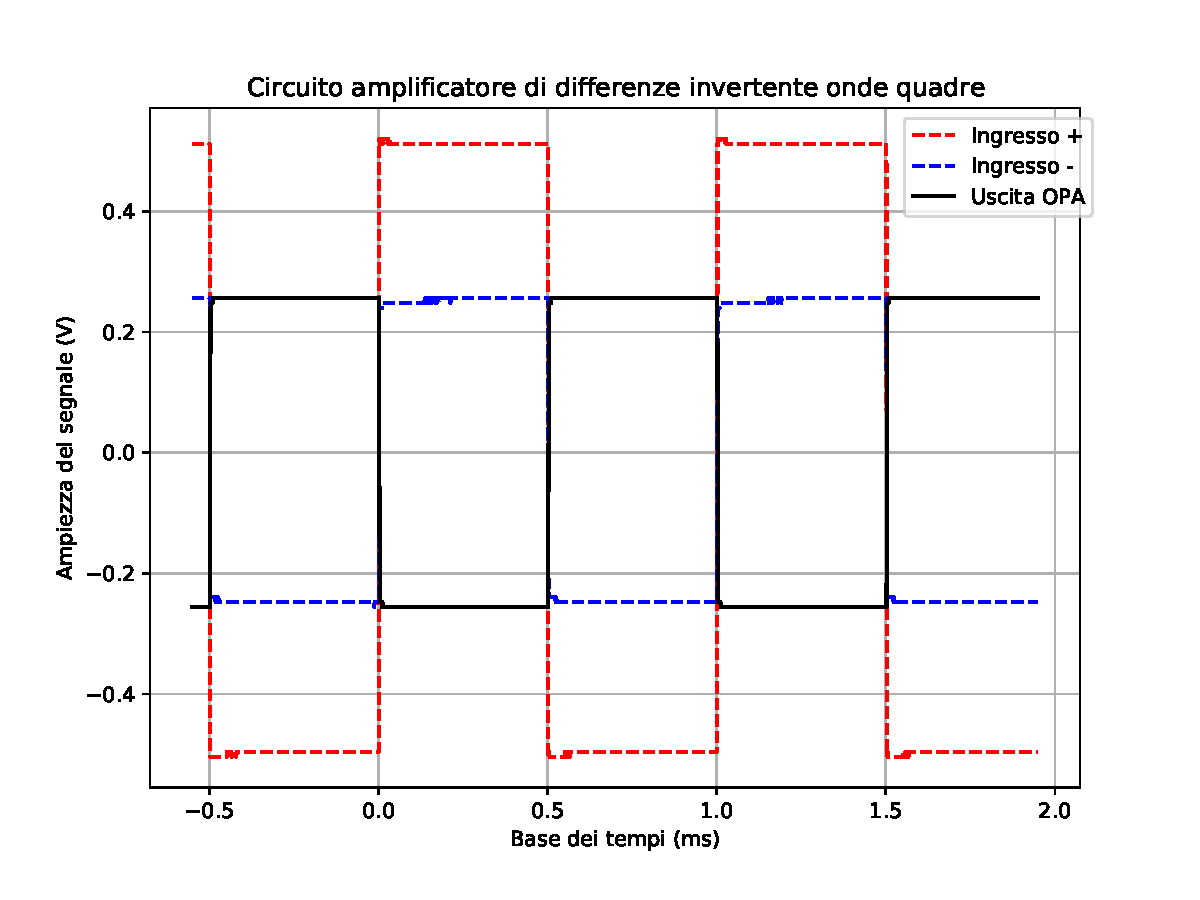
\includegraphics[width=0.45\textwidth]{analysis/output/OPA_diff_square.pdf}
\caption{Sottrazione da un'onda quadra di ampiezza $2A$ di un'onda quadra con ampiezza $A$}
\label{fig:diff_square}
\end {center}
\end{figure}

\vspace{-5mm}

\begin{figure}[H]%[!ht]
\begin {center}
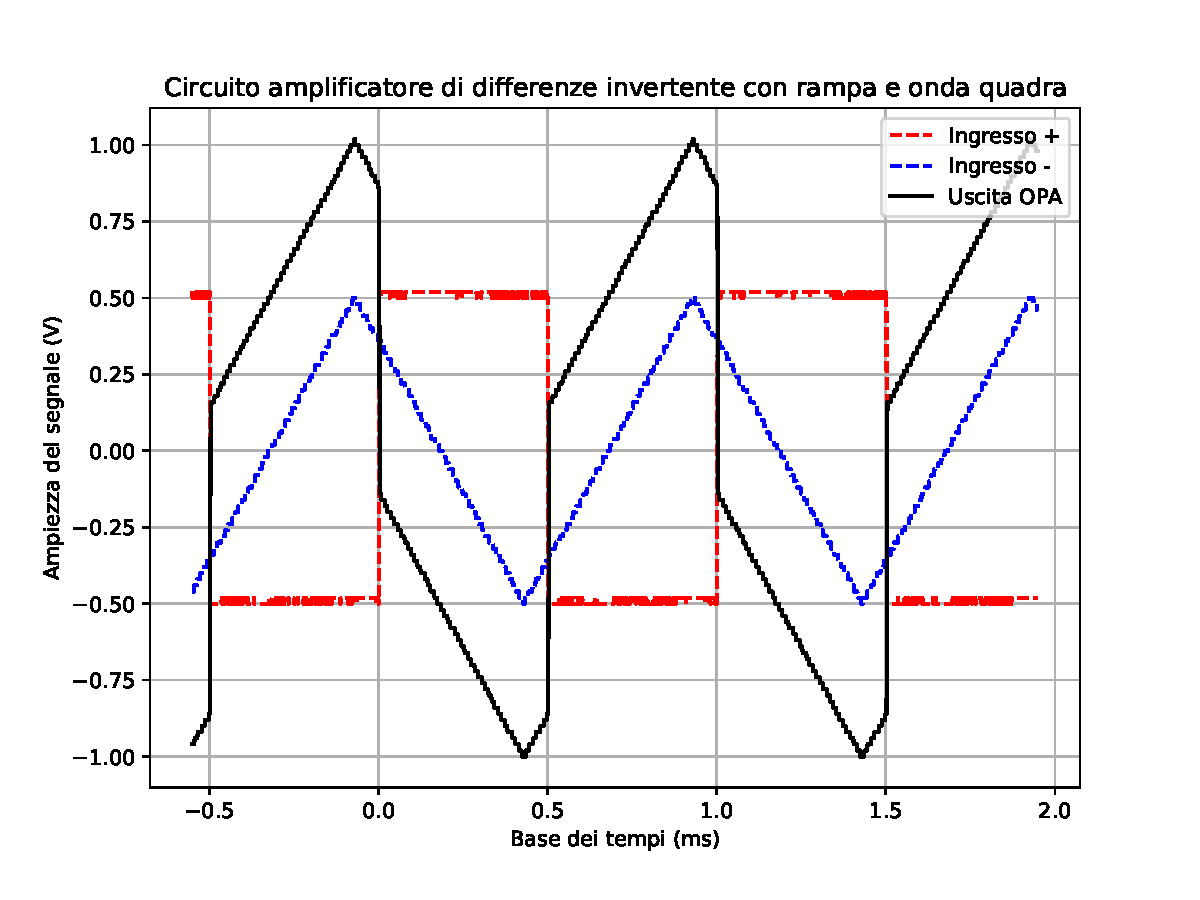
\includegraphics[width=0.45\textwidth]{analysis/output/OPA_diff_squareramp.pdf}
\caption{Differenza tra un'onda quadra e una rampa}
\label{fig:diff_squareramp}
\end {center}
\end{figure}

\vspace{-15mm}

\begin{figure}[H]%[!ht]
\begin{center}
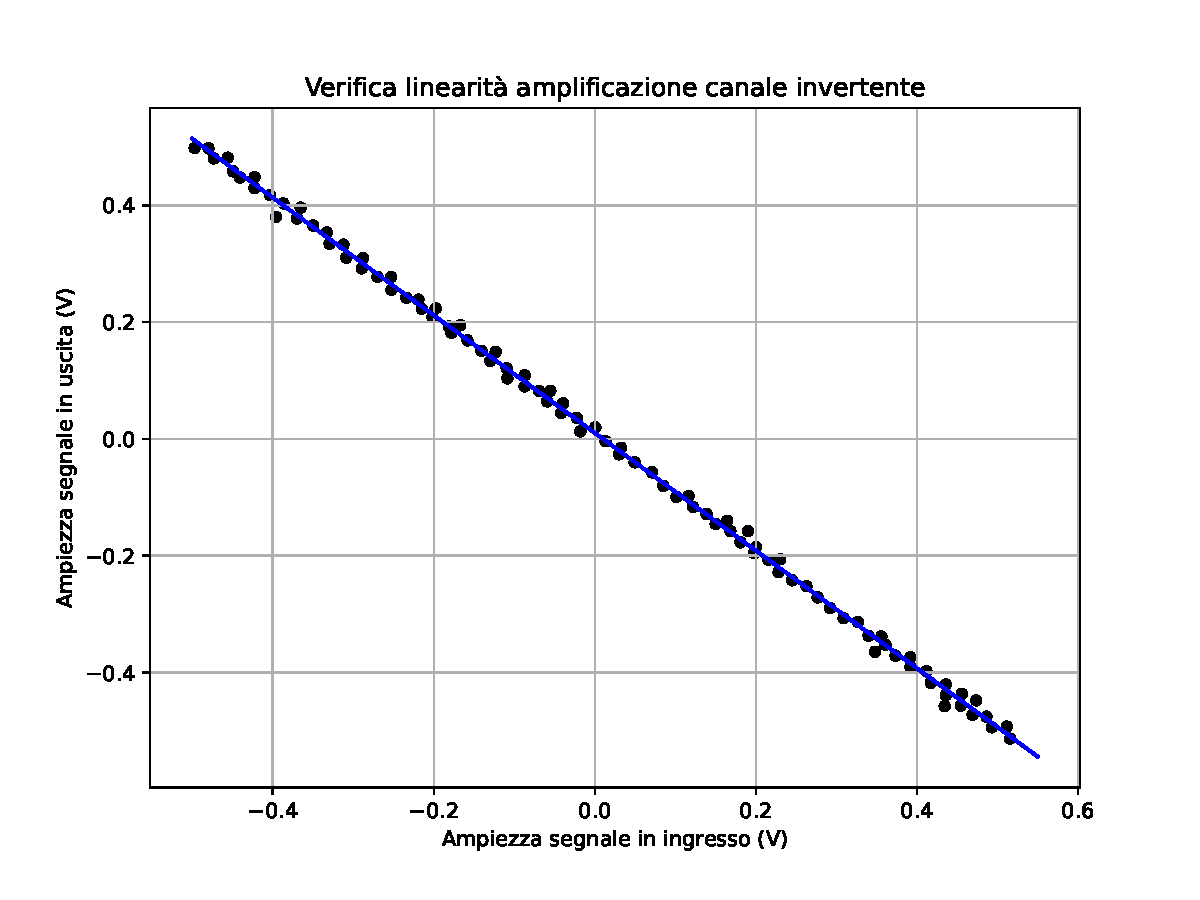
\includegraphics[width=0.45\textwidth]{analysis/output/OPA-linfit-inv.pdf}
\caption{La regressione lineare ($y$ = $ax$ +$b$) del canale invertente in modalità $X-Y$ dell'oscilloscopio ($Ch_in-Ch-out$) restituisce i parametri a = (-1.007 $\pm$ 0.004) e b = (0.010 $\pm$ 0.001) V. La compatibilità del primo valore con 1 conferma il valore atteso per il guadagno.}
\label{fig:lin-inv}
\end{center}
\end{figure}


Con la medesima procedura adoperata nel caso del mixer si è effettuata la verifica della linearità dell'amplificazione del canale invertente effettuando una regressione lineare $V_o = aV_i + b$ sui dati registrati in modalità $X-Y$ di tra il canale invertente e l'uscita.
In questo caso dato che la curva positiva sarà rappresentata dall'ingresso in sottrazione, mentre quella positiva dall'ingresso non in sottrazione ci si aspetta un valore negativo di coefficiente angolare $a_e = -1$

Ancora una volta il parametro $a$ restituito dal minimizzatore risulta essere compatibile con il valore atteso ($Z=1.91$) > $Z_{critico}$ per $\alpha$ = 5 \%, mentre il test di adattamento di $\chi^2$ riporta p-value $\sim$ 1, mostrando che nel range scelto l'amplificatore risulta priva di distorsioni, al livello di accuratezza disponibile con nostri strumenti.


%%%%%%%%%%%%%%%%%%%%%%%%%%%%%%%%%%%%%%%%%%
\section{\textbf{Trigger di Schmitt}} 
\subsection{\textbf{Introduzione}}
Il \textit{Trigger di Schmitt} è un circuito elettronico comparatore che impone isteresi alla soglia di transizione con l'aiuto di un feedback positivo. L'isteresi fa si che vengano forniti due diversi livelli di tensione di soglia per il fronte di salita e di discesa. 
Essenzialmente, si tratta di un multivibratore bistabile, quindi se il segnale in ingresso non attraversa una delle soglie la sua uscita rimane in uno degli stati stabili indefinitamente. Il feedback positivo permette inoltre di avere fronti di commutazione più ripidi rispetto ad un discriminatore ad anello aperto. Per la sua capacità di filtrare il rumore da un segnale digitale viene anche detto \textit{comparatore rigenerativo}.
Le tensioni a cui avviene la commutazione possono essere controllate attraverso i valori di $R_1$ e $R_2$.

\begin{equation}
    V_{th \pm} = \pm \frac{V_{sat}R_2}{R_1+R_2}
\end{equation}

Dove $V_{th+}$ la tensione di soglia superiore e $V_{th-}$ quella inferiore, mentre $V_{sat}$ è la tensione di saturazione. In laboratorio, utilizzando due amplificatori operazionali LM741 è stato implementato il circuito in \textit{Fig. \ref{fig:schmitt-trigger}}. Nel nostro setup sperimentale con $R_1$ = (9.8 $\pm$ 0.1) $\Omega$ e $R_2$ = (9.9 $\pm$ 0.1) $\Omega$ si sono ottenuti, come atteso, valori per soglie $\sim$ $\pm$ $V_{sat}$ / 2 $\sim$ $\pm$ 7.5 V. Infatti, mediante i cursori dell'oscilloscopio è stato misurato $\Delta V_t  = V_{th+}-V_{th-}$ $=$ $(14.42 \pm 0.04) $ $V$ e $\Delta V_{sat}  = V_{sat_+}-V_{sat_{-}}$ $=$ $(28.3 \pm 0.1)$ $ V$

\begin{figure}[H]%[!ht]
\begin{center}
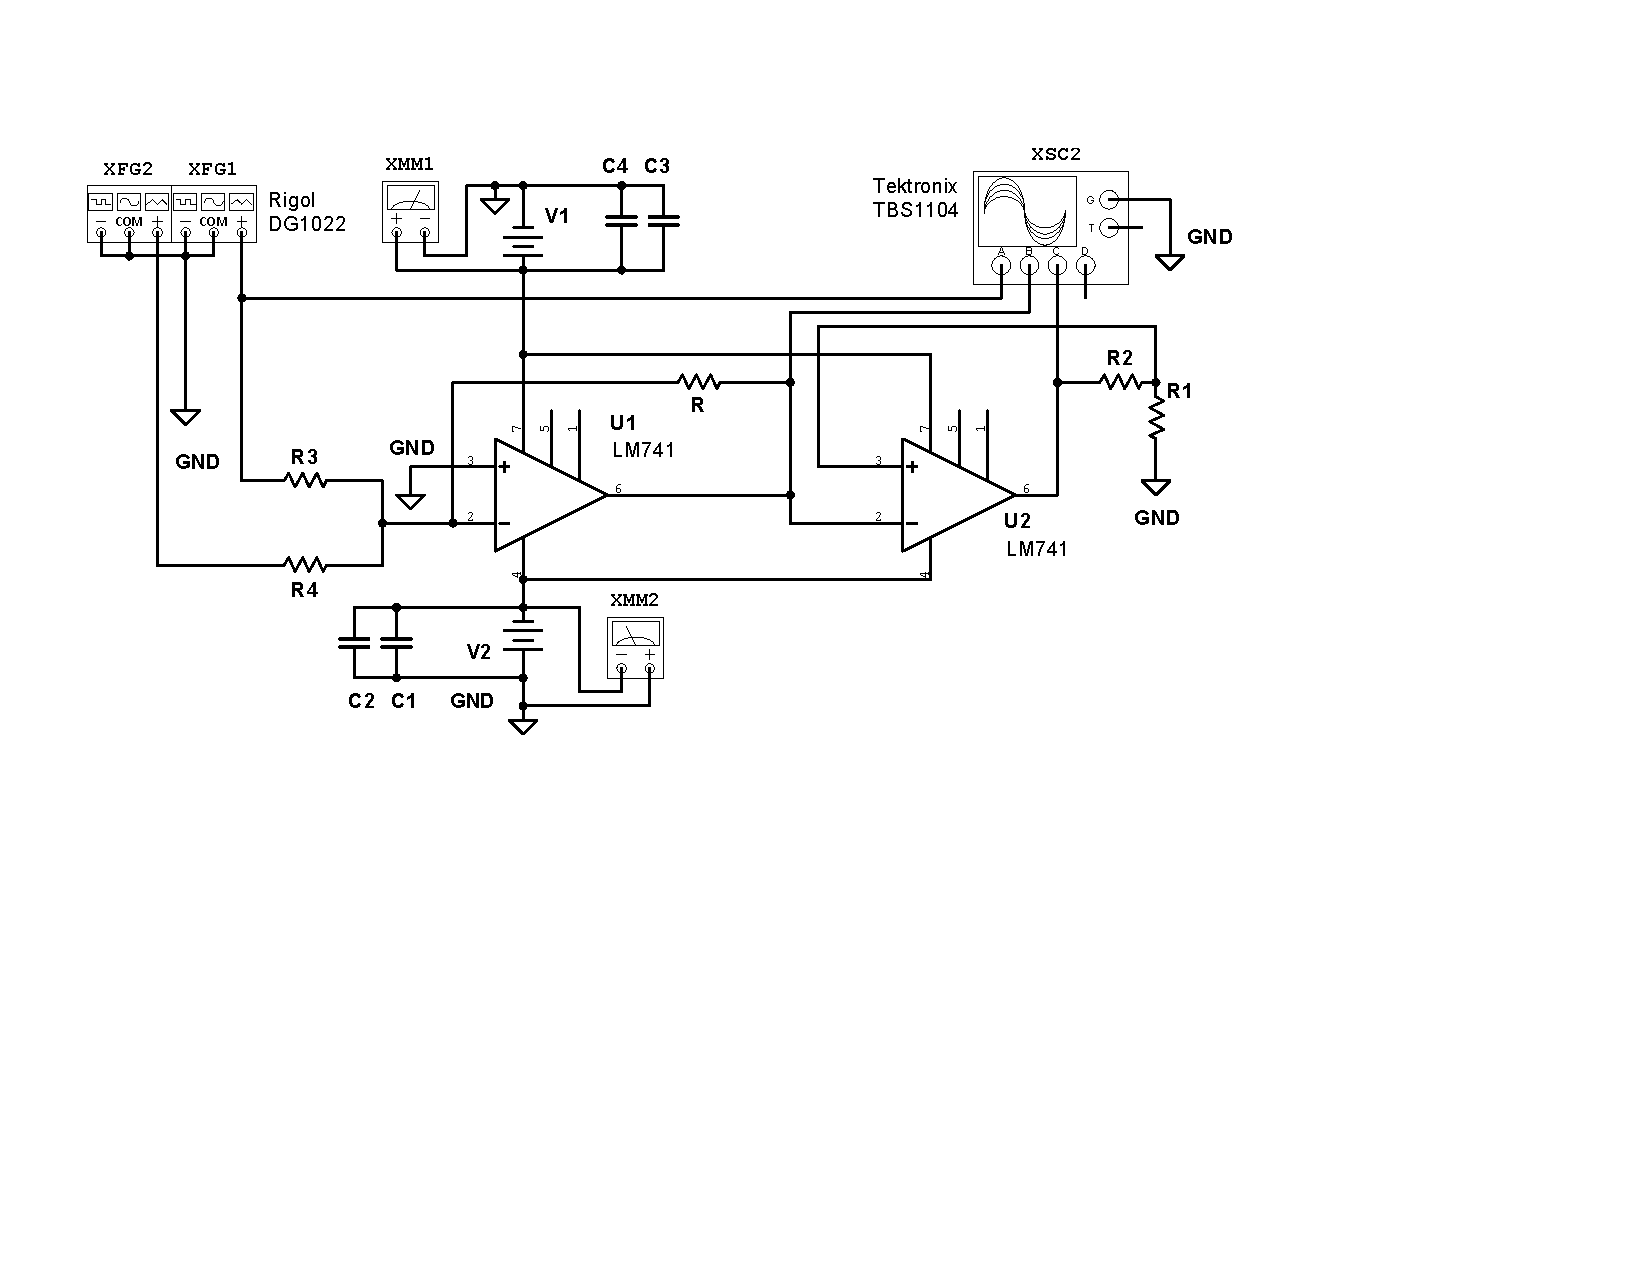
\includegraphics[width=0.45\textwidth]{sch-simulations/output/OPA-mixer-trigger.pdf}
\caption{Schema elettrico utilizzato per la caratterizzazione del trigger di Schmitt con l'obiettivo di mostrare le capacità di immunità al rumore. Il circuito di dotato di due stadi operazionali, il primo con funzione di sommatore produce un segnale rumoroso sommando un noise ad alta frequenza ad un segnale sinusoidale, il secondo costituisce il trigger vero e proprio. Sono stati usati i seguenti valori per le resistenze: $R_1 =(9.8 \pm 0.1) \ k\Omega, \ R_2 = (9.9 \pm 0.1) \ k\Omega ,\ R_3 = (9.8 \pm 0.1) \ k\Omega \, \ R_4 = (9.8 \pm 0.1) \ k\Omega \ R = (9.8 \pm 0.1) \ k\Omega , \ R = (9.8 \pm 0.1 ) \ k\Omega $  } 
\label{fig:schmitt-trigger}
\end{center}
\end{figure}

\subsection{\textbf{Caratterizzazione}}

\begin{figure}[H]%[!ht]
\begin {center}
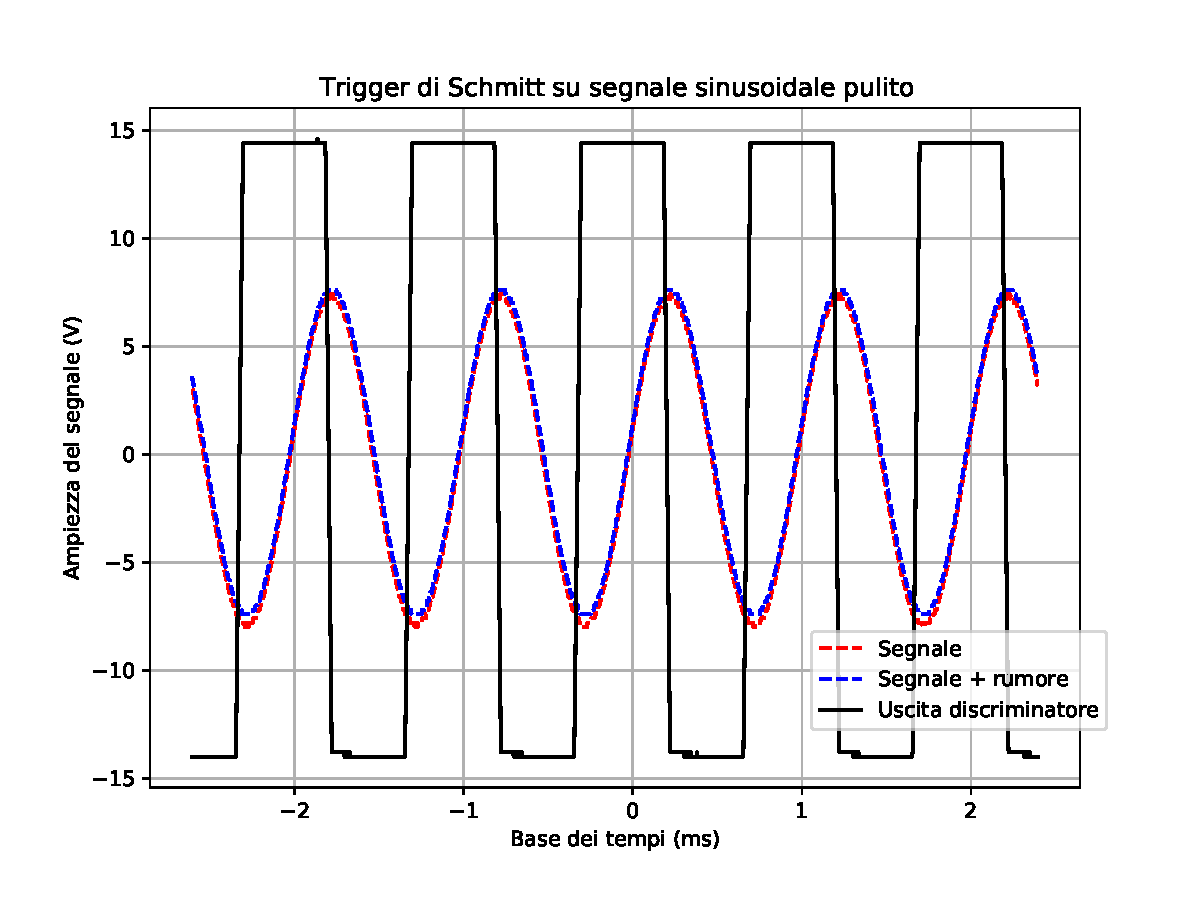
\includegraphics[width=0.50\textwidth]{analysis/output/trigger-pulito.pdf}
\caption{Trigger di Schmitt (con isteresi) a cui viene fornito in ingresso un segnale sinusoidale con rumore trascurabile}
\label{fig:trigger-clean}
\end {center}
\end{figure}


\begin{figure}[H]%[!ht]
\begin {center}
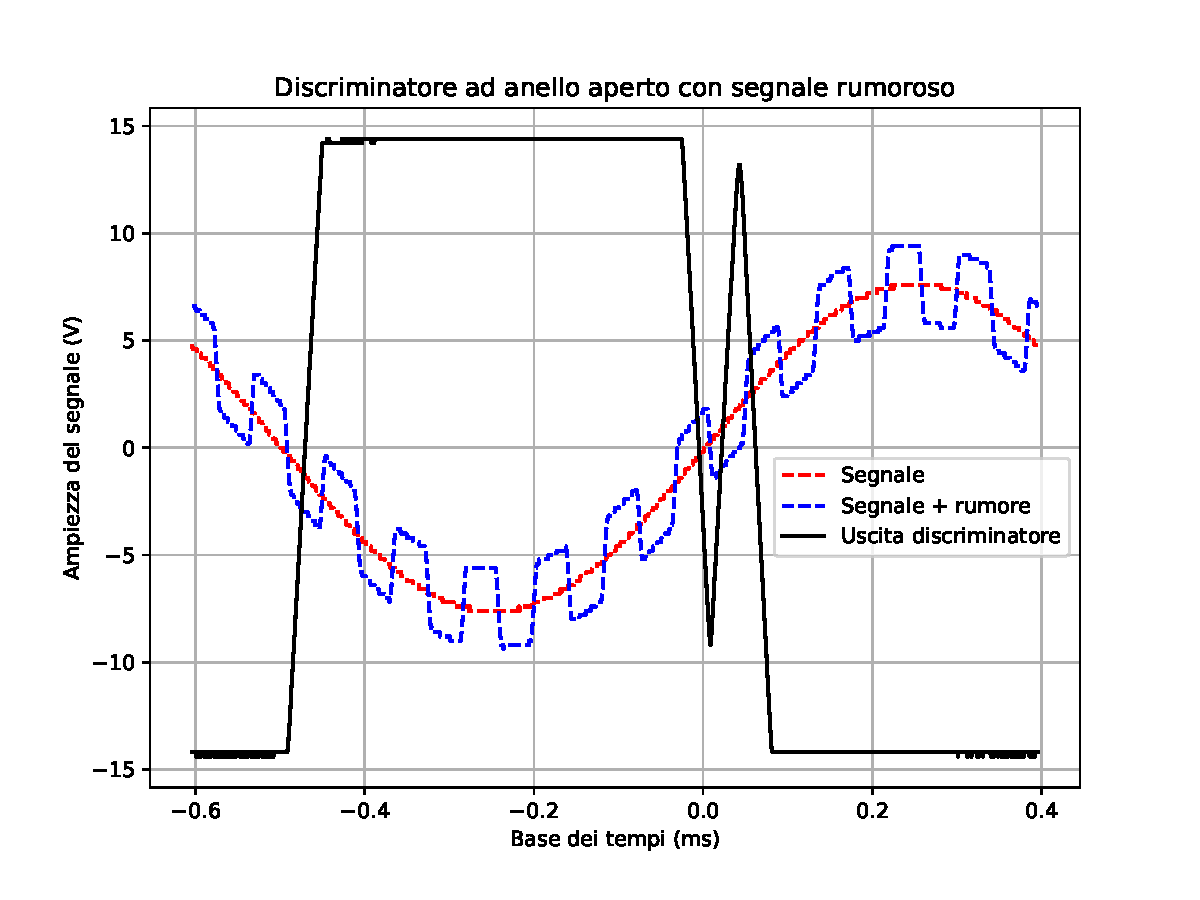
\includegraphics[width=0.50\textwidth]{analysis/output/noisy-open-ring.pdf}
\caption{Discriminatore ad anello aperto (senza isteresi) a cui viene fornito in ingresso un segnale sinusoidale con rumore, si nota una commutazione indesiderata dovuta allo zero-crossing del rumore (soglia = 0 $V$)}
\label{fig:trigger-noisy}
\end {center}
\end{figure}

Inizialmente è stato fornito al \textit{trigger di Schmitt} un segnale sinusoidale con rumore trascurabile, osservando la commutazione invertente con isteresi attesa (\textit{Fig.\ref{fig:trigger-clean}}): 
Un simile circuito può essere utilizzato per trasformare un segnale sinusoidale in un'onda quadra, oppure come già anticipato, per rigenerare dal rumore un segnale digitale.
Nel circuito implementato la tensione di saturazione, riferita a massa è: $+V_{sat}  = 14.6 \pm 0.1  V $ e $-V_{sat}  = -14.0 \pm 0.1  V $. 

In laboratorio si volevano confrontare le capacità di immunità al rumore di un trigger di Schmitt rispetto ad un normale comparatore di soglia realizzato con un amplificatore operazionale in configurazione ad anello aperto. E' quindi stato generato un segnale costituito da una sinusoide con ampiezza $V_{s-pp}$ = 15 V a cui è stato sommato un rumore ad alta frequenza con forma onda quadra di ampiezza $V_{n-pp}$ = 4 V utilizzando un primo stadio operazionale in configurazione mixer invertente. L'uscita di questo stadio è stata dapprima inviata in un comparatore di soglia con $V_{th}$ = 0 ottenendo una serie di commutazioni indesiderate nei punti di \textit{zero-crossing} del rumore, (figura \ref{fig:trigger-noisy}), dopodiché il comparatore è stato sostituito con un trigger di Schmitt e questa volta la commutazione è risultata corretta e immune al rumore, come ben visibile in \textit{figura \ref{fig:trigger-ok}}.


\begin{figure}[H]%[!ht]
\begin {center}
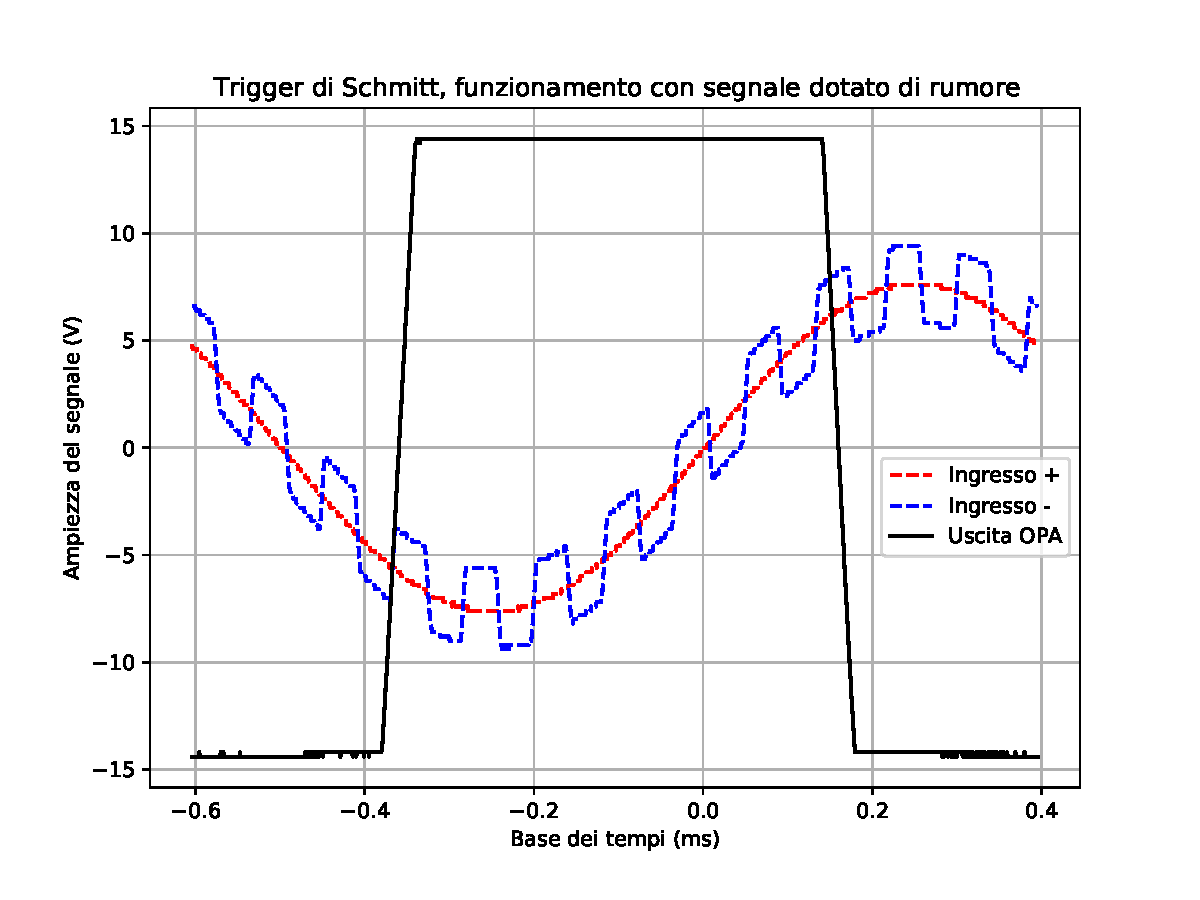
\includegraphics[width=0.50\textwidth]{analysis/output/trigger2.pdf}
\caption{Trigger di Schmitt (con isteresi) a cui viene fornito in ingresso un segnale sinusoidale con rumore, si nota che a differenza del discriminatore ad anello aperto, questo circuito non effettua commutazioni indesiderate sullo zero-crossing del rumore (centraggio della finestra = 0)}
\label{fig:trigger-ok}
\end {center}
\end{figure}

\subsection{Comportamento al variare della frequenza}

\begin{figure}[H]%[!ht]
\begin {center}
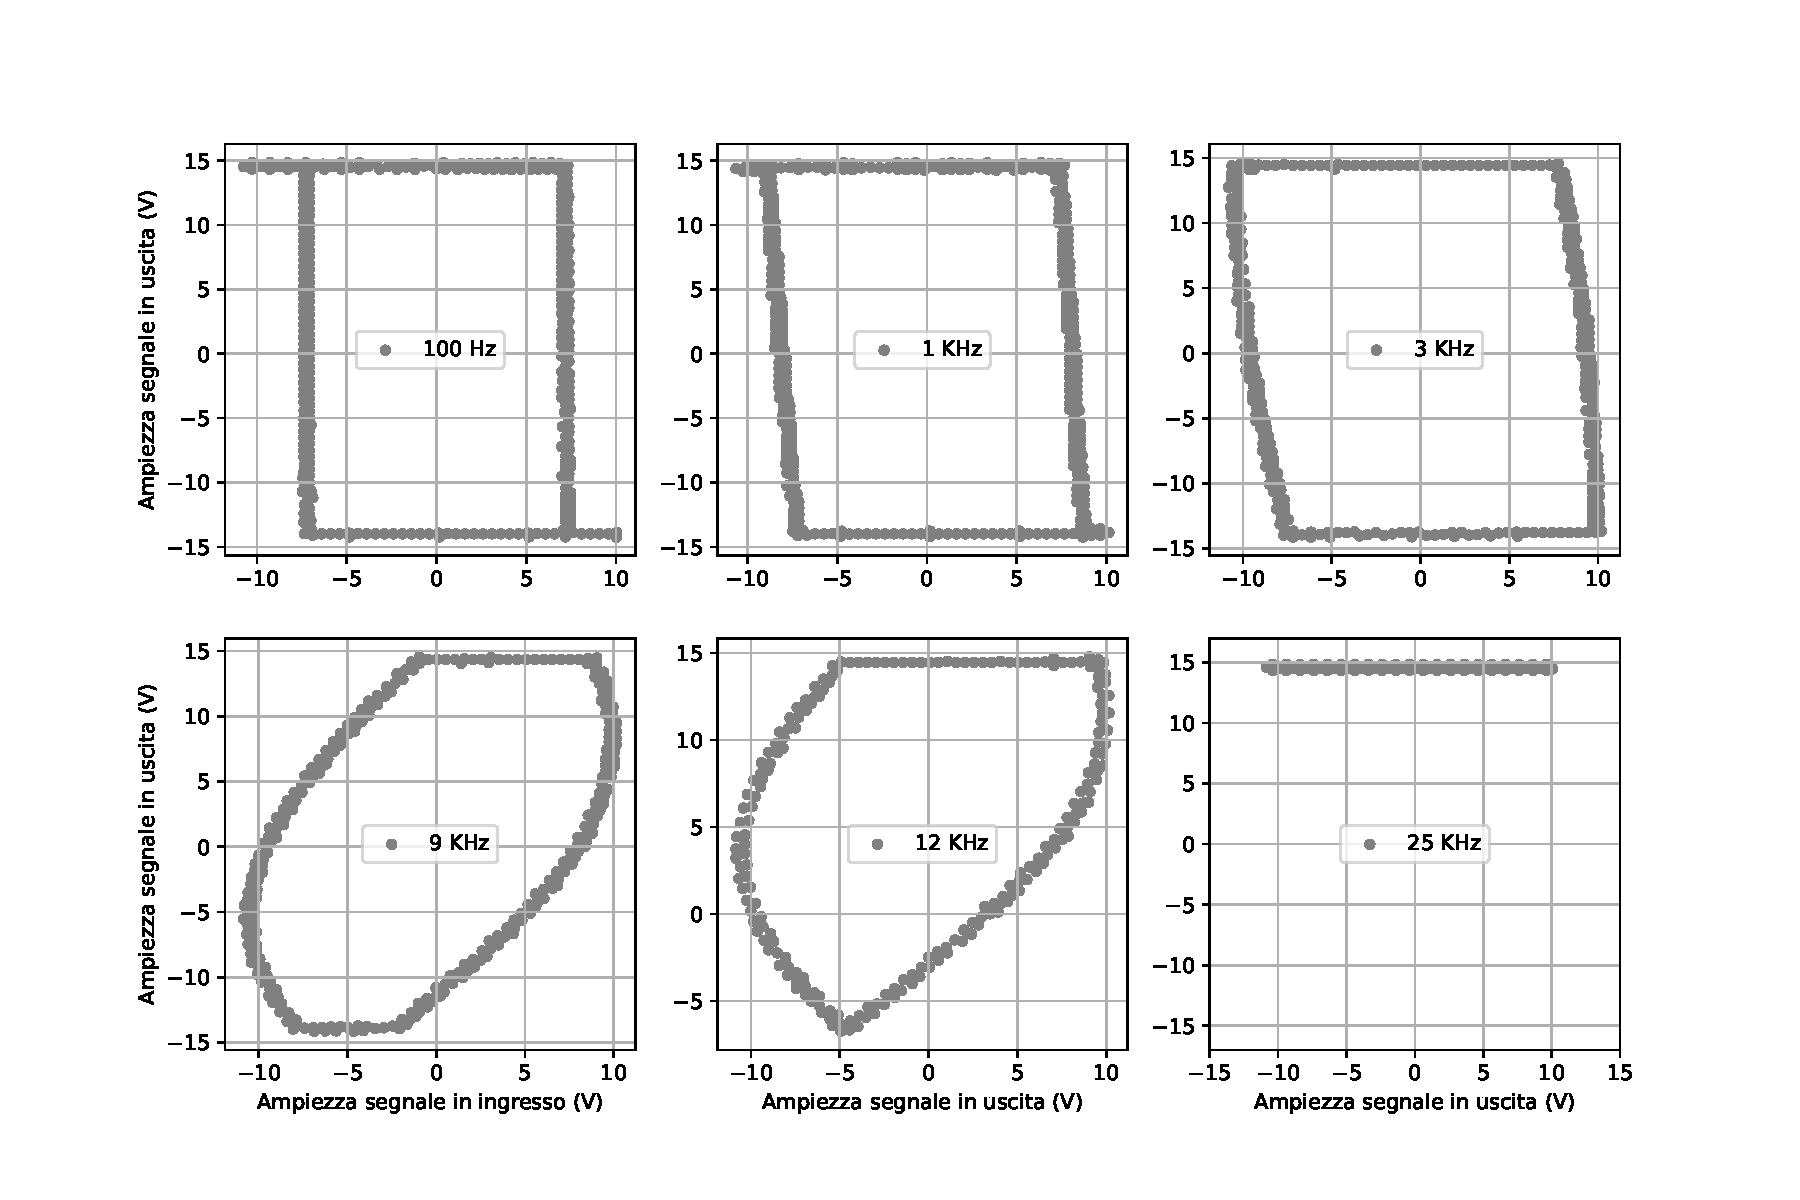
\includegraphics[trim = {30pt 0 0 0}, width=0.50\textwidth]{analysis/output/OPA-trigger-histeresis-table.pdf}
\caption{Rappresentazione dei cicli di isteresi del trigger di Schmitt al variare della frequenza della sinusoide fornita in ingresso. Si osserva chiaramente che ad alta frequenza la velocità di commutazione del circuito diventa insufficiente. Questo parametro dipende dallo slew rate dell'amplificatore operazionale utilizzato.}
\label{fig:hyst-table}
\end {center}
\end{figure}


Terminiamo questa sezione dedicata al trigger di Schmitt volendo verificare la dipendenza delle prestazioni dalla frequenza del segnale fornito in ingresso. Osservando la risposta a $100 Hz$, essa risulta completamente coerente con il comportamento visto prima sul piano tensione-tempo; aumentando la frequenza, però, ci si aspetta che la frequenza di commutazione possa diventare troppo veloce per permettere al trigger di raggiungere in uscita le tensioni di saturazione, dando origine alle situazioni che si osservano in \textit{figg. \ref{fig:hyst-table} e \ref{fig:trigger-hyst}}. Questo fenomeno non è dovuto alla banda passante dell'operazionale, ma bensì al suo slew-rate insufficiente.



\begin{figure}[H]%[!ht]
\begin {center}
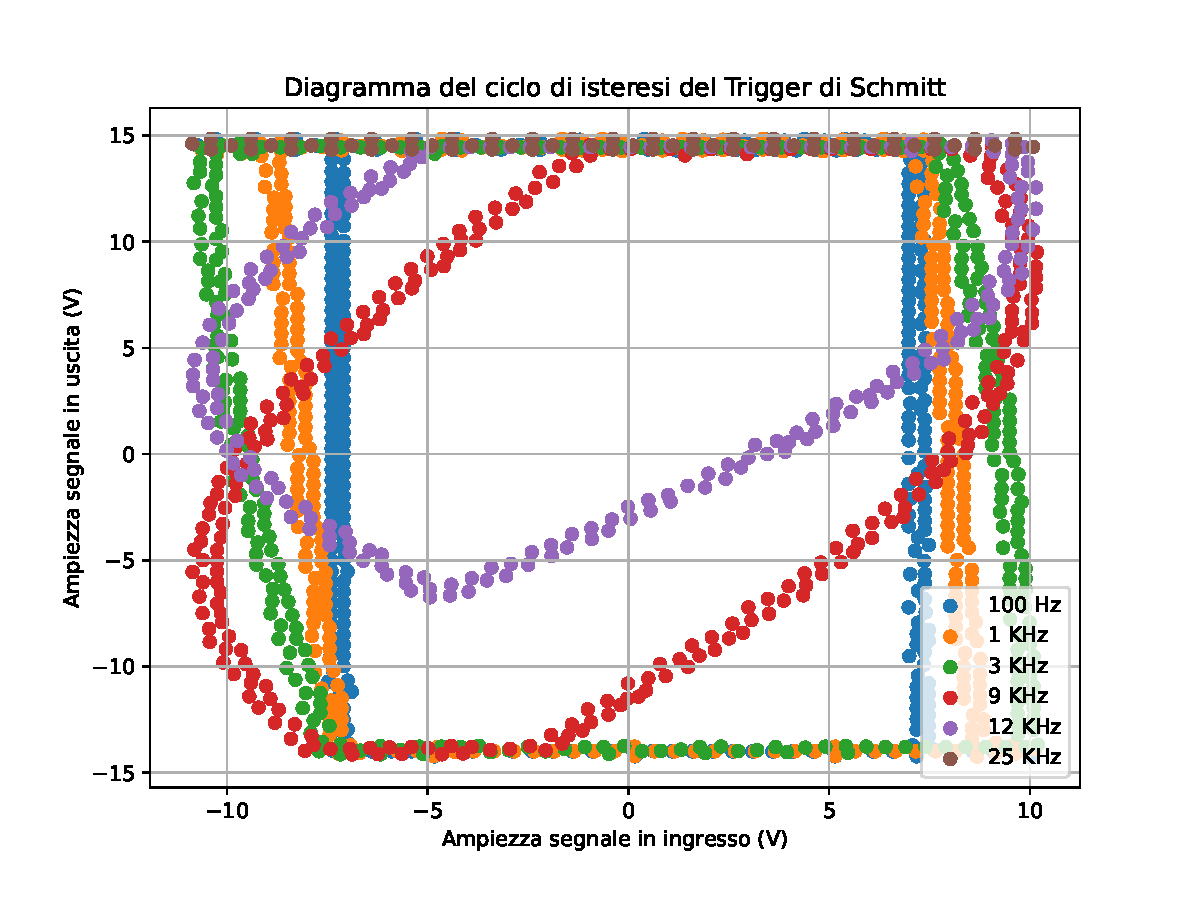
\includegraphics[width=0.50\textwidth]{analysis/output/OPA-trigger-histeresis-overlapped.pdf}
\caption{Sovrapposizione dei grafici rappresentanti i cicli di isteresi a diverse frequenze}
\label{fig:trigger-hyst}
\end {center}
\end{figure}

%%%%%%%%%%FINE TERZO GIORNO%%%%%%%%%%%%%%%%%%
%%%%%%%%%%INIZIO QUARTO GIORNO%%%%%%%%%%%%%%%

%%%%%%%%%%%%%%%%%%%%%%%%%%%%%%%%%%%%%%%%%%
\section{\textbf{Silicon photomultipliers (SiPMs)}} %Valerio
In questa esperienza di laboratorio studieremo qualitativamente il segnale prodotto da un fotomoltiplicatore al silicio illuminato da una sorgente LED. I fotomoltiplicatori al silicio sono fotorivelatori composti da una matrice di SPAD (Single Photon Avalanche Diode) connessi in serie a una resistenza di \textit{quenching} (spegnimento) e collegati in parallelo tra loro. Quando un singolo fotone colpisce il SiPM con una probabilità pari all'efficienza quantica si genera una valanga nello SPAD colpito che provoca un passaggio di corrente dovuto allo scaricamento della capacità di giunzione della cella che provoca una caduta di tensione al catodo (fronte di salita veloce del segnale), al termine della valanga la capacità torna a caricarsi dando origine ad un fronte di discesa più lento. I SiPM sono ampiamente utilizzati per osservare sorgenti di radiazione estremamente deboli o impulsive (anche a livello di singoli fotoni), per esempio nella lettura di rivelatori a scintillazione.

\subsection{\textbf{Circuito per la caratterizzazione del SiPM}}
In laboratorio è stata effettuata una semplice caratterizzazione di due SiPM AdvanSiD NUV: ASD-NUV1S-P e ASD-NUV3S-P \cite{I} caratterizzati da un'efficienza di rilevazione del 43 \%, celle SPAD di dimensione 40x40 $\mu$m, costante di tempo di 70 ns, risposta spettrale tra 350 a 900 nm e guadagno atteso da datasheet di 3.6 $\cdot 10^6$. I due modelli si distinguono per la diversa dimensione della matrice: per il primo 1x1 $mm^2$ (625 celle), mentre per il secondo 3x3 $mm^2$ (5520 celle). Solitamente questi fotorivelatori sono letti in corrente utilizzando un amplificatore transimpedenza, nel nostro caso però si è scelto di impiegare un circuito più semplice, reso possibile dall'elevata sensibilità dell'oscilloscopio Rhode \& Schwarz impiegato (fino a 1 mV/div). Il SiPM è stato alimentato con una tensione di polarizzazione di (30.31 $\pm$ 0.16) V ($\sim +4$ overvolt, tensione di breakdown $\sim$ 26 V) utilizzando l'alimentatore stabilizzato da laboratorio attraverso tre resistenze di limitazione della corrente come illustrato nello schema seguente, con l'aggiunta di un condensatore di livellamento C1 per ridurre l'eventuale \textit{ripple} dell'alimentazione. Per minimizzare i disturbi esterni la tensione è stata portata dall'alimentatore al circuito mediante un cavo coassiale anziché due cavi di potenza con connettori "a banana". I segnali sono stati portati all'oscilloscopio mediante due condensatori di disaccoppiamento per isolare dalla tensione di \textit{biasing} e i canali sono stati sottratti (essendo tra di loro speculari); questo ha permesso di cancellare parzialmente il rumore dell'alimentazione e di aumentare il \textit{SNR}. Il SiPM è stato illuminato con un led rosso pilotato dal generatore \textit{Siglent SDG1010}.

\begin{figure}[H]%[!ht]
\begin{center}
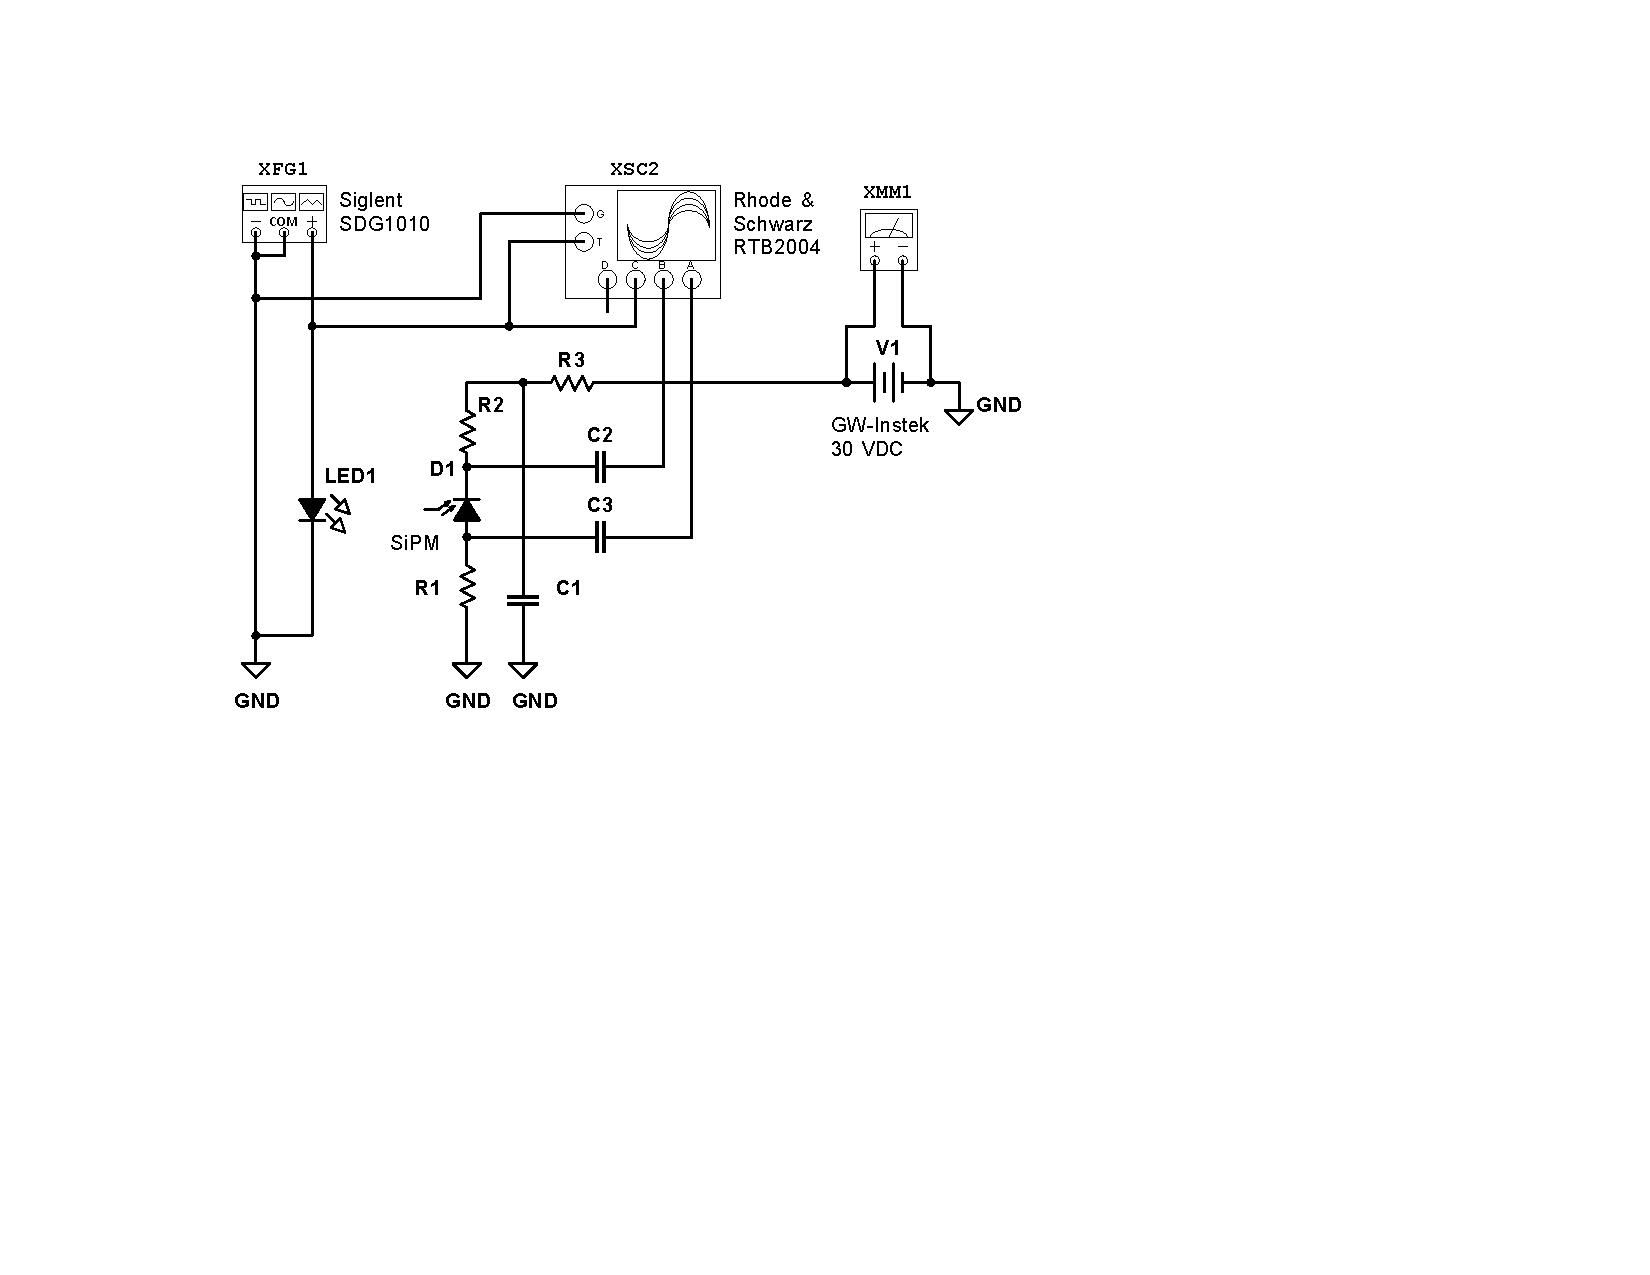
\includegraphics[width=0.46\textwidth]{sch-simulations/output/SiPM.pdf}
\caption{Schema del circuito elettrico per la caratterizzazione del SiPM. Valori per i componenti utilizzati misurati con il multimetro: R1 = (506 $\pm$ 9) $\Omega$, R2 = (513 $\pm$ 9) $\Omega$, R3 = (0.97 $\pm$ 0.01) k$\Omega$, C1 = (90 $\pm$ 7) $nF$, C2 = (98 $\pm$ 8) $nF$, C3 = (94 $\pm$ 7) $nF$}
\label{fig:oscilloscope}
\end{center}
\end{figure}

\subsection{\textbf{Funzionamento in saturazione}}
Per prima cosa si è proceduto a registrare l'impulso il condizione di saturazione per entrambi i SiPM, cioè l'impulso in uscita prodotto quando tutte le celle vengono eccitate, (dove il numero di celle eccitate è proporzionale al numero di fotoni rivelati). Per studiare questo aspetto è stata aumentata l'ampiezza dell'impulso di pilotaggio del LED fino a 5.200 V (durata $\Delta$t = 16 ns, periodo di ripetizione $T$ = 200 ns), i risultati sono presentati nei grafici in figura \ref{fig:SiPM_sat_1mm} e \ref{fig:SiPM_sat_3mm} rispettivamente. Notiamo come l'impulso del SiPM di dimensioni maggiori sia più prolungato, di ampiezza maggiore e più rumoroso, questi effetti sono conseguenza naturale di un numero maggiore di celle SPAD, in particolare la maggiore durata è dovuta ad una più elevata capacità parassita dovuta alla presenza di molte più celle in parallelo.


\begin{figure}[H]%[!ht]
\begin{center}
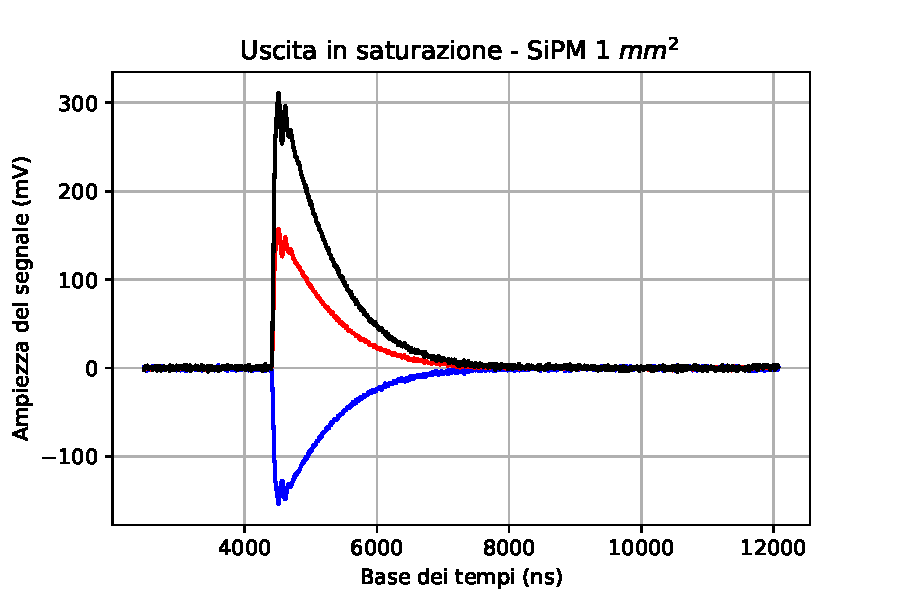
\includegraphics[width=0.40\textwidth]{analysis/output/SiPM_sat_1mm.pdf}
\caption{Segnale prodotto dal SiPM 1x1 $mm^2$ in saturazione: in rosso la tensione all'anodo, il blu la tensione al catodo, il nero la differenza calcolata dall'oscilloscopio.}
\label{fig:SiPM_sat_1mm}
\end{center}
\end{figure}

\begin{figure}[H]%[!ht]
\begin{center}
\includegraphics[width=0.40\textwidth]{analysis/output/SiPM_sat_3mm.pdf}
\caption{Segnale prodotto dal SiPM 3x3 $mm^2$ in saturazione: in rosso la tensione all'anodo, il blu la tensione al catodo, il nero la differenza calcolata dall'oscilloscopio.}
\label{fig:SiPM_sat_3mm}
\end{center}
\end{figure}

\subsection{\textbf{Valutazione del guadagno e del tempo di carica caratteristico}}
In questa fase, più delicata, si vuole invece valutare il guadagno di ciascuna cella e calcolare il tempo caratteristico di carica, dipendente dalla resistenza totale della cella e dalla capacità parassita, che compongono una rete RC. Per raggiungere questo obiettivo si vuole visualizzare una sovrapposizione di impulsi dovuti dall'attivazione di esattamente 1, 2, 3, ... N celle e poter calcolare la differenza in tensione tra i picchi di questi impulsi. Si configura allora il generatore il modo da produrre impulsi di bassissima intensità (stesse impostazioni di prima, ma con $V_{pp}$ = 1.8 mV), si veda la figura \ref{fig:ledp}, in modo che ciascun impulso produca un numero esiguo di fotoni che provocherà l'accensione di poche celle, secondo un modello poissoniano e impostiamo correttamente la persistenza delle tracce sull'oscilloscopio. Si ottengono così i grafici nelle figure \ref{fig:staircase_1mm} e \ref{fig:staircase_3mm} per i due SiPM. 

\begin{figure}[H]%[!ht]
\begin{center}
\includegraphics[width=0.40\textwidth]{analysis/output/SiPM_ledp.pdf}
\caption{Segnale utilizzato per il pilotaggio del led con il SiPM 1x1 $mm^2$ per la misurazione del guadagno}
\label{fig:ledp}
\end{center}
\end{figure}

\begin{figure*}[t]%[t]
\centering
\begin{center}
\includegraphics[trim = {100pt 0 0 0}, width=1.15\textwidth]{analysis/output/SiPM_1mm_gain_staircase.pdf}
\end{center}
\caption{A destra l'istantanea catturata dallo schermo dell'oscilloscopio, a sinistra le tracce estratte numericamente sovrapposte con i cursori orizzontali corrispondenti alle tensioni di picco per l'attivazione di N celle. Il gradiente di colore rappresenta invece la densità di tracce. SiPM 1x1 $mm^2$}
\label{fig:staircase_1mm}
\end{figure*}

\begin{figure*}[t]%[t]
\centering
\begin{center}
\includegraphics[trim = {100pt 0 0 0}, width=1.15\textwidth]{analysis/output/SiPM_3mm_gain_staircase.pdf}
\end{center}
\caption{Come nella figura precedente, ma questa volta per il SiPM di dimensioni 3x3 $mm^2$}
\label{fig:staircase_3mm}
\end{figure*}

A partire da tali tracce sono stati ricavati i valori di tensione di picco per ciascun impulso corrispondente ad un determinato numero di celle con metodi numerici, i dati sono riportati in appendice. Dopo aver calcolato le differenze tra ogni valore e il successivo, si è provveduto ad effettuare una media e a calcolare l'incertezza stimandola con la semidispersione massima. Abbiamo così trovato come 'quanto' di tensione corrispondente ad una cella attivata $\Delta V_{1mm}$ = (0.21 $\pm$ 0.02) $mV$ e  $\Delta V_{3mm}$ = (0.13 $\pm$ 0.02) $mV$. (Questi valori sono già stati divisi per due, rispetto ai grafici, dal momento che provengono dalla somma dei canali.) Si è quindi potuta calcolare la quantità di carica immagazzinata in ciascuna cella $Q$, considerando la sua modellizzazione sopracitata come capacità ideale. Per un condensatore in un circuito con costante di tempo $\tau$ si ha che la carica totale immagazzinata è
\begin{equation}
    Q = \int_{0}^{\infty} i(t) dt = \int_{0}^{\infty} \frac{\Delta V}{Z} e^{-t/ \tau}  dt = \frac{\Delta V}{Z} \tau
\end{equation}

con $Z = 50 \Omega$. (Il calcolo dei valori di $\tau$ è descritto nel paragrafo seguente). Per trovare il guadagno si divide ora la carica Q per la carica elementare dell'elettrone, trovando così il fattore di moltiplicazione dovuto all'effetto valanga caratteristico dello SPAD. Il calcolo restituisce $G_{1mm} = (2.9 $\pm$ 0.3)\cdot 10^6$ e $G_{3mm} = (2.9 $\pm$ 0.4)\cdot 10^6$. I valori ottenuti risultano entrambi compatibili con quanto atteso sulla base del \textit{datasheet} del produttore AdvanSiD, che riporta per un overvolt di +4 ($V_{bias} = V_{breakdown} + 4$) G $\sim$ 3$\cdot10^6$. I pvalue del test Z di compatibilità con tale riferimento sono infatti rispettivamente di 0.821 e 0.865, ampiamente superiori del livello di significatività standard del test $\alpha = 0.05$.

\subsection{\textbf{Calcolo della costante di tempo}}
Nel paragrafo precedente per poter calcolare la carica Q è stato fondamentale disporre della costante di tempo $\tau$ per i circuiti RC formati dalle resistenze di quenching e dalle capacità delle giunzioni degli SPAD (collegati in parallelo). Verrà ora discussa la tecnica adottata per il calcolo delle $\tau$. Secondo l'approssimazione totalmente ideale presentata, la costante di tempo non dipende dall'ampiezza degli impulsi, quindi per lavorare con un miglior rapporto segnale / rumore, si decide di lavorare sugli impulsi in saturazione (fig. \ref{fig:SiPM_sat_1mm} e \ref{fig:SiPM_sat_3mm}) descritti nei paragrafi precedenti. Gli impulsi sono stati ritagliati sull'asse temporale e poi sono stati interpolati con la legge di scarica del condensatore dopo aver aggiunto opportuni parametri aggiuntivi per considerare l'offset arbitrario degli assi e l'ampiezza dell'impulso non nota:
\begin{equation}
    V(t) = V_0 e^{-(t-t_0)/\tau} + V_{offset}
\end{equation}
Entrambi i fit hanno esito positivo, considerando un test $\chi^2$ solo sulla coda destra (pvalue $\sim$ 1), si ottengono infatti valori di $\chi^2 / NDF$ pari a 11.51  /  300 = 0.038 per il SiPM con area minore e $\chi^2 / NDF$ pari a 102.46 /  300 = 0.341 per quello con area maggiore. E' possibile finalmente estrarre il parametro di interesse (con la relativa incertezza, dalla matrice di covarianza) ottenendo $\tau_{1mm}$ = (1.11 $\pm$ 0.02)$\cdot 10^{-7}$ s e $\tau_{3mm}$ = (1.88 $\pm$ 0.10)$\cdot 10^{-7}$ s. Le figure \ref{fig:fit1m} e \ref{fig:fit3m} mostrano l'esito delle interpolazioni. Nei calcoli si è adottata come incertezza sulle tensioni misurate con l'oscilloscopio 1/5 della larghezza delle divisioni verticali.

\begin{figure}[H]%[!ht]
\begin{center}
\includegraphics[width=0.38\textwidth]{analysis/output/SiPM_fit_3mm.pdf}
\caption{Interpolazione dell'impulso in saturazione del SiPM 1x1 $mm^2$ per estrapolare la costante di tempo caratteristica.}
\label{fig:fit1m}
\end{center}
\end{figure}

\begin{figure}[H]%[!ht]
\begin{center}
\includegraphics[width=0.38\textwidth]{analysis/output/SiPM_fit_1mm.pdf}
\caption{Interpolazione dell'impulso in saturazione del SiPM 3x3 $mm^2$ per estrapolare la costante di tempo caratteristica.}
\label{fig:fit3m}
\end{center}
\end{figure}

\subsection{\textbf{Discussione e considerazioni conclusive}}
In conclusione, la metodologia sperimentale proposta è risultata adeguata per effettuare una misurazione indicativa del guadagno e della costante di tempo di fotomoltiplicatori al silicio. L'utilizzo dell'oscilloscopio con un segnale di trigger esterno prodotto dal generatore è risultato fondamentale, in quanto ha permesso di eliminare gran parte degli eventi dovuti al dark count che avrebbero disturbato la misura. Le acquisizioni qualitative sono risultate in accordo con quanto atteso, il SiPM da 3x3 $mm^2$ ha infatti mostrato una maggior sensibilità, una maggiore quantità di rumore e una costante di tempo più elevata a causa della capacità di un numero maggiore di celle in parallelo  rispetto a quello con area 1x1 $mm^2$. I valori ottenuti risultano ampiamente compatibili con i quanto riportato sul \textit{datasheet}, ma l'accuratezza potrebbe essere migliorabile con varie strategie. Innanzitutto si potrebbe cercare di ridurre ulteriormente gli impulsi di rumore isolando in modo più efficace il SiPM dalla luce ambientale, dopodiché si potrebbe calcolare la carica specifica associata a ciascuno SPAD integrando numericamente la forma d'onda dell'impulso oppure con un amplificatore di carica, eliminando la necessità di introdurre un'approssimazione di idealità con la legge (1). Questo metodo basato sulla misura diretta della carica potrebbe risultare più robusto rispetto a quello attuale basato sulla misura di tensioni. Il metodo di misura delle costanti di tempo basato sull'interpolazione è risultato molto più efficace rispetto all'uso di cursori, come confermato dai test Z di compatibilità con quanto riportato sul \textit{datasheet} e dai test di adattamento di $\chi^2$.

%%%%%%%%%%%%%%%%%%%%%%%%%%%%%%%%%%%%%%%%%%
\section{\texbf{Linea di ritardo}} %Federico

Un segnale che si propaga lungo un cavo coassiale subisce un'attenuazione dovuta alla resistività del materiale del conduttore e la sua velocità di propagazione dipende dalle induttanze e dalle capacità caratteristiche dei conduttori che costituiscono la linea. Ciò produce, nei cavi reali, un'impedenza caratteristica della linea $Z_c$, dipendente esclusivamente dal materiale di cui è composto il cavo e dalla sua geometria.
Considerando un tratto infinitesimo $\delta x$ del cavo (\textit{fig. \ref{fig:coassiale}) }, si può impostare un sistema di due equazioni differenziali del tipo:

\begin{equation}
    \begin{cases}
  \frac{dV}{dx} = -Z_1 I \\
  \frac{dI}{dx} = -V Y_2 
\end{cases} 
\end{equation}

Definendo $\gamma = (Z_1 Y_2)^{1/2}$ (costante della propagazione della linea) e $Z_c = (Z_1 Z_2)^{1/2}$ (impedenza caratteristica) ed integrando si ottiene:
 \begin{equation}
     V(x) = Ae^{-\gamma x} + Be^{\gamma x}
 \end{equation}
 \begin{equation}
     I(x) = (1/Z_c)(Ae^{-\gamma x} + Be^{\gamma x}) 
 \end{equation}
Le espressioni ricavate dipendono solo da $x$ e non dal tempo. 
Quello che si osserva è che il segnale è la risultante di un'onda diretta, che si attenua con l'aumentare delle $x$ e un'onda riflessa che pare aumentare in ampiezza al crescere delle $x$ e che dunque viaggia in senso opposto. Risulta utile defnire la quantità $\rho = (Z_L / Z_c + 1) - (Z_L / Z_c - 1)$, dove $Z_L$ la resistenza di carico.

\begin{figure}[H]%[!ht]
\begin {center}
\includegraphics[width=0.38\textwidth]{analysis/output/cavo coassiale.png}
\caption{Tratto $\delta x$ cavo assiale}
\label{fig:coassiale}
\end {center}
\end{figure}

Supponiamo ora di chiudere la linea con un'impedenza di carico $Z_L$, si potranno configurare tre possibili situazioni: 
\begin{itemize}
    \item $Z_L = 0$ (cortocircuito, $\rho = -1$): il segnale riflesso ha la stessa ampiezza di quello incidente ed è capovolto
    \item $Z_L = \infty$ (circuito aperto, $\rho = 1$): il segnale riflesso torna al generatore con ampiezza doppia rispetto a quello trasmesso
    \item $Z_L = Z_c$ (linea adattata, $\rho = 0$): non c'è segnale riflesso, il segnale incidente si attenua all'infinito.
\end{itemize}

I valori tipici per un cavo coassiale tipo RG-58 e RG-174 sono $Z_c = 50 \Omega \ $ con ritardo di propagazione per metro $  \ 1/v_f = 5 \ ns/m $.

\begin{figure*}[h]%[t]
\centering
\begin{center}
\includegraphics[trim = {150pt 0 0 0}, width=1.1\textwidth]{analysis/output/Delay_line_pulse.pdf}
\caption{Linea di ritardo, misure a tempo di volo con singolo impulso}
\label{fig:singolo impulso}
\end{center}
\end{figure*}


\subsection{\textbf{Setup sperimentale e misura del tempo di volo  di un impulso singolo}}
E' stato fornito un cavo coassiale di lunghezza totale $L$ incognita, suddiviso in una parte lunga $L/2$ e due parti lunghe $L/4$. Ad uno dei capi è stato collegato il generatore di segnali Keithley 3390. I canali dell'oscilloscopio sono stati collegati all'ingresso e alternativamente al primo quarto, a metà e all'uscita del cavo. (fig. \ref{fig:linea di ritardo}). Il cavo (RG-58) era intestato con connettori BNC.
La linea poteva essere chiusa alternativamente con una resistenza di valore pari all'impedenza caratteristica, cioè $50 \Omega$, con un cortocircuito o poteva essere lasciata aperta.

\begin{figure}[H]%[!ht]
\begin {center}
\includegraphics[width=0.38\textwidth]{sch-simulations/output/Transmission line.pdf}
\caption{Schema circuitale per testare la linea di ritardo. R1A è l'eventuale resistenza di terminazione.}
\label{fig:linea di ritardo}
\end {center}
\end{figure}

Per verificare qualitativamente il comportamento della linea nei tre casi descritti, per ognuna delle terminazioni possibili e effettuare una prima stima della lunghezza L della linea è stato inviato un treno di impulsi di durata pari a 20 ns, con fronti di salita e di discesa larghi 5 ns e frequenza di ripetizione in questo caso pari a $1 kHz$. Il segnale veniva acquisito sui canali 1 e 2 dell'oscilloscopio rispettivamente all'inizio e alla fine della linea di lunghezza L incognita. \textit{(fig. \ref{fig:singolo impulso})}.


\begin{itemize}
    \item Nel primo caso - terminazione in corto circuito - il segnale riflesso è capovolto rispetto al segnale incidente, dunque all'uscita l'oscilloscopio registra una tensione molto piccola (prossima a 0), mentre si osserva un impulso capovolto che si propaga verso l'ingresso;
    \item Nel secondo caso - terminazione con circuito aperto - sull'uscita di osserva un segnale di ampiezza circa uguale a quella originale, solamente attenuato dalla resistività dei conduttori (dipendente a sua volta dalla frequenza), mentre si osserva all'ingresso un impulso di ritorno di altezza doppia rispetto a quello originale.
    \item Il terzo caso si ottiene installando alla terminazione della linea un carico resistivo di $50 \Omega$, pari all'impedenza caratteristica, il quale fa si che il segnale non venga riflesso e la linea di comporti per il generatore come se fosse di lunghezza infinita.
\end{itemize}
 

Nel caso a circuito aperto, è possibile stimare la lunghezza $L$ del cavo, misurando il tempo di andata e ritorno dell'impulso: sapendo che il segnale si propaga a velocità $v_f = 5 \ ns$. Il valore $\Delta t / {v_f}$ corrisponde infatti al doppio della distanza percorsa dal segnale. 
Estrapolando dal grafico del segnale in ingresso i valori per i due massimi relativi che corrispondono alla partenza e al ritorno dell'impulso, si calcola $\Delta t$. Si ottiene quindi: 
$L = (27.7 \pm 0.5) \ m $. (Errore stimato tenendo conto sia della risoluzione temporale dell'oscilloscopio, sia dell'imprecisione di posizionamento dei cursori dovuta a forme differenti dei fronti di salita).


\subsection{\textbf{Periodo di ripetizione}}

\begin{figure}[H]%[!ht]
\begin{center}
\includegraphics[width=0.5\textwidth]{analysis/output/Delay_line_repetition.pdf}
\caption{Linea di ritardo, condizione di minimo in cui l'impulso di ritorno si somma in opposizione di fase con quello in partenza dando origine ad una risultante minima (in nero).}
\label{fig: ripetizione di impulsi}
\end{center}
\end{figure}


E' possibile effettuare una misura più raffinata della lunghezza del cavo inviando, anziché un singolo impulso, una ripetizione di impulsi ad un intervallo costante, pari al periodo di andata-ritorno dell'impulso, partendo dalla stima ottenuta con la tecnica a tempo di volo. Nella configurazione con l'uscita in cortocircuito, l'onda riflessa - opposta a quella incidente - annullerà quest'ultima in prossimità del generatore, portando ad una tensione risultante sul canale 1 dell'oscilloscopio minima. Questa condizione si realizza con un periodo di ripetizione pari a $\tau = (267.2 \pm 0.1)$ $ns$, con questo metodo si è ottenuto un valore di lunghezza pari a $ L = $ $(27.6 \pm 0.1)$ $m $. La condizione di minimo dell'impulso risultante qui descritta è stata ottenuta minimizzando il valore $V_{pp}$ e in figura \ref{fig: ripetizione di impulsi} è possibile osservare quanto acquisito con l'oscilloscopio.



Come si nota il segnale risultante è minimizzato, ma non è del tutto trascurabile, cioè dovuto a fenomeni di attenuazione dipendente dalla frequenza e dispersione all'interno della linea di trasmissione che deformano leggermente gli impulsi durante il trasporto.
La misura ottenuta con il secondo metodo risulta essere ampiamente compatibile con quella ottenuta a tempo di volo. Un test Z di Gauss riporta un p-value $\sim 1$.


\begin{figure*}[h]%[t]
\centering
\begin{center}
\includegraphics[trim = {200pt 0 0 0}, width=1.1\textwidth]{analysis/output/Delay_line_standingWave2L.pdf}
\caption{Onde stazionarie con lunghezza d'onda $\lambda = 2L$}
\label{fig: "onde staz 2L}
\end{center}
\end{figure*}

\begin{figure*}[h]%[t]
\centering
\begin{center}
\includegraphics[trim = {200pt 0 0 0}, width=1.1\textwidth]{analysis/output/Delay_line_standingWaveL.pdf}
\caption{Onde stazionarie con lunghezza d'onda $\lambda = L$}
\label{fig: onde staz L}
\end{center}
\end{figure*}


\begin{figure*}[h]%[t]
\includegraphics[trim = {200pt 0 0 0}, clip, width=1.1\textwidth]{analysis/output/Delay_line_lambda2L.pdf}
\caption{Onde stazionarie nella linea di trasmissione con lunghezza d'onda $\lambda = 2L$}
\label{fig: delayline 2L}

\end{figure*}

\begin{figure*}[h]%[t]
\includegraphics[trim = {200pt 0 0 0}, clip, width=1.1\textwidth]{analysis/output/Delay_line_lambdaL.pdf}
\caption{Onde stazionarie nella linea di trasmissione con lunghezza d'onda $\lambda = L$}
\label{fig: delayline L}
\end{figure*}



\subsection{\textbf{Formazione di onde stazionarie}}

Se al posto di un impulso si invia sulla linea un segnale sinusoidale con lunghezza d'onda pari a quella della linea oppure pari al suo doppio (o altre armoniche) si generano delle onde stazionarie risultanti dall'interferenza dell'onda incidente con quella riflessa. 
In un'onda stazionaria le posizioni dei ventri (interferenza costruttiva) e dei nodi (interferenza distruttiva) sono costanti nel tempo e il tipo di armonica che si formerà dipende da come viene terminata la linea.



Prendiamo ora in esame i grafici in \textit{(figg. \ref{fig: "onde staz 2L} e \ref{fig: onde staz L})} che mostrano l'andamento teorico di fronti d'onda di onde stazionarie nelle tre possibili configurazioni della linea.
La linea con terminazione a circuito aperto si comporta come una cavità risonante ad estremità aperte; quella a terminazione con cortocircuito come una cavità risonante ad estremità chiuse. Nel caso di linea adattata non essendoci onda riflessa non si generano onde stazionarie. Nei due grafici si distingue anche il comportamento nel caso di lunghezza d'onda pari a $L$ e $2L$: ciò che cambia è il numero di ventri e nodi che si formano in quanto si forma un'armonica di ordine differente. I risultati sono presentati nelle figure \ref{fig: delayline 2L} e \ref{fig: delayline L}. In particolare per il caso $\lambda$ = 2L osserviamo che, come atteso:
\begin{itemize}
    \item Con circuito aperto: il fronte d'onda ha un nodo (V=0) a $L/2$ e ventri (massimi e minimi) in $0 \ e\ L$, mentre a $L/4$ l'ampiezza è attenuata 
    \item Con cortocircuito sull'uscita: il fronte d'onda ha nodi a $0\ e\ L$ e un ventre in $L/2$, mentre a $L/4$ l'ampiezza è attenuata
    \item Con linea adattata: non c'è onda riflessa, l'onda si propaga senza interferenze.
\end{itemize}
Invece con $\lambda$ = L :
\begin{itemize}
    \item Con circuito aperto: Si ottengono massimi su ingresso, uscita e a L/2, in questo caso in controfase, e minimo a L/4
    \item Con cortocircuito sull'uscita: Si ottengono minimi sull'ingresso, sull'uscita e un massimo a L/4
    \item Con linea adattata: non c'è onda riflessa, l'onda si propaga senza interferenze.
\end{itemize}

\subsection{Conclusioni}
Dallo studio del comportamento di una linea di ritardo con diverse terminazioni - cortocircuito, circuito aperto e linea adattata - è stata ricavata la misura della lunghezza del cavo utilizzato sia tramite l'invio di un singolo impulso sia con ripetizioni di impulsi. Inviando onde sinusoidali si è verificata qualitativamente la formazione di onde stazionarie nella linea e, per ciascuna delle terminazioni, si è studiato il comportamento dei fronti d'onda ad inizio, $L/4, \ L/2$, ed $L$. 



%%%%%%%%%%%%%%%%%%%%%%%%%%%%%%%%%%%%%%%%%%
\section{Conclusioni generali} %Tutti quanti
In questa breve relazione di laboratorio sono stati caratterizzati alcuni circuiti nell'ambito dell'elettronica analogica che ricoprono particolare importanza nella ricerca in fisica. I risultati ottenuti sono risultati globalmente in accordo con la teoria, come è stato possibile verificare qualitativamente attraverso i grafici, oppure in alcuni casi quantitativamente mediante test statistici di compatibilità tra i valori ottenuti in laboratorio e quanto predetto dai modelli utilizzati. Le metodologie impiegate sono risultate adeguate, in particolare è sempre risultato possibile raggiungere nelle misure un rapporto segnale / rumore sufficiente per poter mettere in luce le caratteristiche desiderate del circuito sotto esame. La breadboard, infatti, nel range di frequenze utilizzato (0 - 1 MHz) non ha mostrato attenuazioni o capacità parassite problematiche. Da questo punto di vista l'esperienza più delicata è risultata la caratterizzazione del SiPM, per cui si rimanda all'apposito paragrafo di discussione. \\

Particolarmente rilevante è risultata la possibilità di esportare le tracce in formati numerici (CSV) dall'oscilloscopio per poter procedere all'analisi in un secondo momento con tecniche più quantitative che hanno garantito maggior precisione (per esempio grazie ad algoritmi di ricerca dei fronti di salita e discesa) rispetto all'uso dei cursori dell'oscilloscopio (posizionamento soprattutto visivo). Questo soprattutto nella misurazione degli intervalli tra impulsi nell'esperienza della linea di ritardo, oppure per la misurazione delle tensioni durante la caratterizzazione del SiPM.

%%%%%%%%%%%%%%%%%%%%%%%%%%%%%%%%%%%%%%%%%%

\clearpage
\section{Appendice}
%INSERIRE:
% 1. Tabella presa dati per ciascun bode plot
% 2. Tabella presa dati 



\begin{table}[H]
\begin{tabular}{c|c|c}
\multicolumn{1}{c|}{$V_{in}$ {[}mV{]}} & \multicolumn{1}{|c|}{$V_{out}$ {[}mV{]}} & \multicolumn{1}{c}{$f$ {[}Hz{]}}\\ 
\hline  \\
104 $ \pm $ 4 & (9.5 $ \pm $ 0.4) $ \cdot 10^{2} $ & 1.000 $ \pm $ 0.001       \\
97 $ \pm $ 4  & (9.4 $ \pm $ 0.4) $ \cdot 10^{2} $ & 5.000 $ \pm $ 0.005         \\
96 $ \pm $ 4  & (9.4 $ \pm $ 0.4) $ \cdot 10^{2} $ & 10.00 $ \pm $ 0.01        \\
96 $ \pm $ 4  & (9.4 $ \pm $ 0.4) $ \cdot 10^{2} $ & 50.00 $ \pm $ 0.05          \\
96 $ \pm $ 4  & (9.4 $ \pm $ 0.4) $ \cdot 10^{2} $ & 250.0 $ \pm $ 0.3         \\
97 $ \pm $ 4  & (9.4 $ \pm $ 0.4) $ \cdot 10^{2} $ & 1000 $ \pm $ 1          \\
96 $ \pm $ 4  & (9.4 $ \pm $ 0.4) $ \cdot 10^{2} $ & 3000 $ \pm $ 3          \\
95 $ \pm $ 4  & (9.4 $ \pm $ 0.4) $ \cdot 10^{2} $ & (1.000 $ \pm $ 0.001)  $ \cdot 10^{4} $            \\
85 $ \pm $ 4  & (8.2 $ \pm $ 0.4) $ \cdot 10^{2} $ & (1.500 $ \pm $ 0.002)   $ \cdot 10^{4} $          \\
89 $ \pm $ 4  & (8.3 $ \pm $ 0.4) $ \cdot 10^{2} $ & (2.500 $ \pm $ 0.003 ) $ \cdot 10^{4} $             \\
82 $ \pm $ 4  & (7.5 $ \pm $ 0.4) $ \cdot 10^{2} $ & (3.000 $ \pm $ 0.003 ) $ \cdot 10^{04} $             \\
87 $ \pm $ 4  & (7.7 $ \pm $ 0.4) $ \cdot 10^{2} $ & (4.000 $ \pm $ 0.004) $ \cdot 10^{4} $   \\
86 $ \pm $ 4  & (7.2 $ \pm $ 0.4) $ \cdot 10^{2} $ & (4.500 $ \pm $ 0.004) $ \cdot 10^{4} $   \\
97 $ \pm $ 4  & (8.2 $ \pm $ 0.4) $ \cdot 10^{2} $ & (5.000 $ \pm $ 0.005) $ \cdot 10^{4} $   \\
89 $ \pm $ 4  & (7.5 $ \pm $ 0.4) $ \cdot 10^{2} $ & (5.500 $ \pm $ 0.005) $ \cdot 10^{4} $   \\
88 $ \pm $ 4  & (6.7 $ \pm $ 0.4) $ \cdot 10^{2} $ & (7.500 $ \pm $ 0.007) $ \cdot 10^{4} $   \\
97 $ \pm $ 4  & (6.3 $ \pm $ 0.4) $ \cdot 10^{2} $ & (1.0000 $ \pm $ 0.0010) $ \cdot 10^{5} $ \\
90 $ \pm $ 4  & (5.6 $ \pm $ 0.4) $ \cdot 10^{2} $ & (1.1000 $ \pm $ 0.0011) $ \cdot 10^{5} $ \\
88 $ \pm $ 4  & (4.9 $ \pm $ 0.4) $ \cdot 10^{2} $ & (1.3000 $ \pm $ 0.0013) $ \cdot 10^{5} $ \\
89 $ \pm $ 4  & (4.3 $ \pm $ 0.4) $ \cdot 10^{2} $ & (1.6000 $ \pm $ 0.0016) $ \cdot 10^{5} $ \\
100 $ \pm $ 4 & (4.0 $ \pm $ 0.4) $ \cdot 10^{2} $ & (2.0000 $ \pm $ 0.0020) $ \cdot 10^{5} $ \\
92 $ \pm $ 4  & (3.0 $ \pm $ 0.4) $ \cdot 10^{2} $ & (2.5000 $ \pm $ 0.0025) $ \cdot 10^{5} $ \\
101 $ \pm $ 4 & (2.8 $ \pm $ 0.4) $ \cdot 10^{2} $ & (3.0000 $ \pm $ 0.0030) $ \cdot 10^{5} $ \\
102 $ \pm $ 4 & (2.2 $ \pm $ 0.4) $ \cdot 10^{2} $ & (4.000 $ \pm $ 0.004) $ \cdot 10^{5} $   \\
102 $ \pm $ 4 & (1.3 $ \pm $ 0.4) $ \cdot 10^{2} $ & (7.000 $ \pm $ 0.007) $ \cdot 10^{5} $   \\
101 $ \pm $ 4 & 86 $ \pm $ 4 & (1.0000 $ \pm $ 0.0010) $ \cdot 10^{6} $ \\
101 $ \pm $ 4 & 41 $ \pm $ 4 & (2.0000 $ \pm $ 0.0020) $ \cdot 10^{6} $ \\
100 $ \pm $ 4 & 12 $ \pm $ 4 & (5.000 $ \pm $ 0.005) $ \cdot 10^{6} $   \\
77 $ \pm $ 4  & 2 $ \pm $ 4  & (2.0000 $ \pm $ 0.0020) $ \cdot 10^{7} $
\end{tabular}
\vspace{5 mm}
\caption{Scala valori di tensione in input e output relativi a frequenze progressive relative all'OPA invertente, guadagno teorico 10}
\label{tab:opa-inv-g10}
\end{table}


\begin{table}[H]
\centering
    
\begin{tabular}{c|c|c}
\multicolumn{1}{c|}{$V_{in}$ {[}mV{]}} & \multicolumn{1}{|c|}{$V_{out}$ {[}mV{]}} & \multicolumn{1}{c}{$f$ {[}Hz{]}}\\ 
\hline  \\
64 $\pm$ 4 & 114 $\pm$ 4 & 1.000 $\pm$ 0.001 \\
62 $\pm$ 4 & 116 $\pm$ 4 & 10.00 $\pm$ 0.01  \\
61 $\pm$ 4  & 121 $\pm$ 4 & 100.0 $\pm$ 0.1  \\
61 $\pm$ 4  & 119 $\pm$ 4 & 1000 $\pm$ 1     \\
61 $\pm$ 4  & 119 $\pm$ 4 & 5000 $\pm$ 5     \\
57 $\pm$ 4  & 112 $\pm$ 4 & (1.300 $\pm$ 0.001) $\cdot 10^4$    \\
62 $\pm$ 4  & 119 $\pm$ 4 & (5.000 $\pm$ 0.005) $\cdot 10^4$    \\
55 $\pm$ 4  & 104 $\pm$ 4 & (1.000 $\pm$ 0.001) $\cdot 10^5$  \\
58 $\pm$ 4  & 106 $\pm$ 4 & (2.000 $\pm$ 0.002) $\cdot 10^5$   \\
53 $\pm$ 4  & 90 $\pm$ 4  & (3.500 $\pm$ 0.004) $\cdot 10^5$   \\
54 $\pm$ 4  & 82 $\pm$ 4  & (5.000 $\pm$ 0.005) $\cdot 10^5$  \\
57 $\pm$ 4  & 78 $\pm$ 4  & (6.000 $\pm$ 0.006) $\cdot 10^5$   \\
54 $\pm$ 4  & 67 $\pm$ 4  & (7.500 $\pm$ 0.008) $\cdot 10^5$   \\
55 $\pm$ 4  & 54 $\pm$ 4  & (1.000 $\pm$ 0.001) $\cdot 10^6$ \\
55 $\pm$ 4  & 34 $\pm$ 4  & (1.700 $\pm$ 0.002) $\cdot 10^6$ \\
57 $\pm$ 4  & 22 $\pm$ 4  & (2.500 $\pm$ 0.003) $\cdot 10^6$\\
57 $\pm$ 4  & 15 $\pm$ 4  & (3.300 $\pm$ 0.003) $\cdot 10^6$ \\
58 $\pm$ 4  & 9 $\pm$ 4   & (5.000 $\pm$ 0.005) $\cdot 10^6$ \\
\end{tabular}
\vspace{5 mm}
\caption{Scala valori di tensione in input e output relativi a frequenze progressive relative all'OPA non invertente}
\label{tab:opa-non-inv}
\end{table}

\begin{table}[H]
\centering

\begin{tabular}{c|c|c}
\multicolumn{1}{c|}{$V_{in}$ {[}mV{]}} & \multicolumn{1}{|c|}{$V_{out}$ {[}mV{]}} & \multicolumn{1}{c}{$f$ {[}Hz{]}}\\ 
\hline  \\
151 $\pm$ 4 & 146 $\pm$ 4 & 1.000 $\pm$ 0.001  \\
144 $\pm$ 4 & 144 $\pm$ 4 & 5.000 $\pm$ 0.005  \\
147 $\pm$ 4 & 146 $\pm$ 4 & 10.00 $\pm$ 0.01   \\
144 $\pm$ 4 & 143 $\pm$ 4 & 50.00 $\pm$ 0.05   \\
144 $\pm$ 4 & 142 $\pm$ 4 & 250.0 $\pm$ 0.3    \\
144 $\pm$ 4 & 142 $\pm$ 4 & 1000 $\pm$ 1       \\
142 $\pm$ 4 & 143 $\pm$ 4 & 3000 $\pm$ 3       \\
142 $\pm$ 4 & 143 $\pm$ 4 & (1.000 $\pm$ 0.001) $\cdot 10^{04}$            \\
142 $\pm$ 4 & 142 $\pm$ 4 & (5.000 $\pm$ 0.005) $\cdot 10^{04}$   \\
142 $\pm$ 4 & 140 $\pm$ 4 & (1.0000 $\pm$ 0.0010) $\cdot 10^{05}$ \\
146 $\pm$ 4 & 138 $\pm$ 4 & (2.0000 $\pm$ 0.0020) $\cdot 10^{05}$ \\
145 $\pm$ 4 & 130 $\pm$ 4 & (3.0000 $\pm$ 0.0030) $\cdot 10^{05}$ \\
145 $\pm$ 4 & 122 $\pm$ 4 & (4.000 $\pm$ 0.004) $\cdot 10^{05}$   \\
146 $\pm$ 4 & 112 $\pm$ 4 & (5.000 $\pm$ 0.005) $\cdot 10^{05}$   \\
146 $\pm$ 4 & 105 $\pm$ 4 & (6.000 $\pm$ 0.006) $\cdot 10^{05}$   \\
\end{tabular}
\vspace{5 mm}
\caption{Scala valori di tensione in input e output relativi a frequenze progressive relative all'OPA invertente, guadagno teorico 1}
\label{tab:opa-inv-g1}
\end{table}


\begin{table}[H]
\centering
    
\begin{tabular}{c|c|c}
\multicolumn{1}{c|}{$V_{in}$ {[}V{]}} & \multicolumn{1}{|c|}{$V_{out}$ {[}V{]}} & \multicolumn{1}{c}{$f$ {[}Hz{]}}\\ 
\hline  \\
81 $\pm$ 4 & 79 $\pm$ 4 & 100.0 $\pm$ 0.1      \\
82 $\pm$ 4 & 78 $\pm$ 4 & 150.0 $\pm$ 0.2     \\
81 $\pm$ 4 & 78 $\pm$ 4 & 200.0 $\pm$ 0.2      \\
81 $\pm$ 4 & 74 $\pm$ 4 & 300.0 $\pm$ 0.3      \\
81 $\pm$ 4 & 69 $\pm$ 4 & 4.0 $\pm$ 0.4      \\
81 $\pm$ 4 & 68 $\pm$ 4 & 4.0 $\pm$ 0.5     \\
81 $\pm$ 4 & 65 $\pm$ 4 & 500.0 $\pm$ 0.5      \\
81 $\pm$ 4 & 57 $\pm$ 4 & 700.0 $\pm$ 0.7      \\
81 $\pm$ 4 & 47 $\pm$ 4 & 1000 $\pm$ 1     \\
81 $\pm$ 4 & 42 $\pm$ 4 & 1200 $\pm$ 1     \\
81 $\pm$ 4 & 35 $\pm$ 4 & 1500 $\pm$ 2     \\
80 $\pm$ 4 & 28 $\pm$ 4 & 2000 $\pm$ 2     \\
80 $\pm$ 4 & 23 $\pm$ 4 & 2500 $\pm$ 3     \\
80 $\pm$ 4 & 19 $\pm$ 4 & 3000 $\pm$ 3     \\
80 $\pm$ 4 & 17 $\pm$ 4 & 3500 $\pm$ 4     \\
80 $\pm$ 4 & 15 $\pm$ 4 & 4000 $\pm$ 4     \\
80 $\pm$ 4 & 12 $\pm$ 4 & 5000 $\pm$ 5     \\
80 $\pm$ 4 & 11 $\pm$ 4 & 5500 $\pm$ 6    \\
80 $\pm$ 4 & 10 $\pm$ 4 & 6000 $\pm$ 6     \\
81 $\pm$ 4 & 9 $\pm$ 4  & 7000 $\pm$ 7     \\
81 $\pm$ 4 & 7 $\pm$ 4  & (1.00 $\pm$ 0.01) $\cdot 10^4$   \\
81 $\pm$ 4 & 6 $\pm$ 4  & (1.40 $\pm$ 0.01) $\cdot 10^4$    \\
81 $\pm$ 4 & 4 $\pm$ 4  & (2.00 $\pm$ 0.02) $\cdot 10^4$    \\
80 $\pm$ 4 & 2 $\pm$ 4  & (5.00 $\pm$ 0.05) $\cdot 10^4$    \\
81 $\pm$ 4 & 2 $\pm$ 4  & (1.00 $\pm$ 0.01) $\cdot 10^5$ 
\end{tabular}
\vspace{5 mm}
\caption{Scala valori di tensione in input e output relativi a frequenze progressive relative all'OPA integratore}
\label{tab:opa-non-inv}
\end{table}

\vfill



\begin{table}[H]
\centering
\begin{tabular}{c|c}
\multicolumn{1}{c|}{$V_{in}$ {[}V{]}} & \multicolumn{1}{c}{$V_{out}$ {[}V{]}} \\ \hline
\\
0.568 $\pm$ 0.004 & -0.548 $\pm$ 0.002  \\
0.880 $\pm$ 0.005 & -0.564 $\pm$ 0.002 \\ 
1.099 $\pm$ 0.006 & -0.577 $\pm$ 0.002 \\ 
1.377 $\pm$ 0.008 & -0.586 $\pm$ 0.002 \\ 
1.642 $\pm$ 0.009 & -0.596 $\pm$ 0.002 \\ 
2.05 $\pm$ 0.01 & -0.605 $\pm$ 0.002 \\ 
2.50 $\pm$ 0.02 & -0.613 $\pm$ 0.002 \\ 
3.04 $\pm$ 0.02 & -0.62 $\pm$ 0.002 \\ 
3.66 $\pm$ 0.02 & -0.627 $\pm$ 0.002 \\ 
4.08 $\pm$ 0.03 & -0.63 $\pm$ 0.007 \\ 
4.62 $\pm$ 0.03 & -0.635 $\pm$ 0.007 \\ 
5.12 $\pm$ 0.04 & -0.638 $\pm$ 0.007 \\ 
5.64 $\pm$ 0.04 & -0.641 $\pm$ 0.007 \\ 
6.24 $\pm$ 0.04 & -0.645 $\pm$ 0.007 \\ 
7.02 $\pm$ 0.05 & -0.648 $\pm$ 0.007 \\ 
7.76 $\pm$ 0.05 & -0.649 $\pm$ 0.007 \\ 
8.48 $\pm$ 0.05 & -0.652 $\pm$ 0.007 \\ 
9.31 $\pm$ 0.06 & -0.653 $\pm$ 0.007 \\ 
10.09 $\pm$ 0.06 & -0.657 $\pm$ 0.007 \\ 
12.31 $\pm$ 0.07 & -0.659 $\pm$ 0.007 \\ 
\end{tabular}
\vspace{5 mm}
\caption{Scala valori di tensione in input e output relativi a frequenze progressive relative all'OPA logaritmico}
\label{tab:opa-log}
\end{table}




\begin{table}[H]
    \centering
    \title{Scala valori di tensione accensione singoli SPAD del SiPM}
    \begin{tabular}{c|c}
    SiPM 1x1 $mm^2$ [$\mu V$]     &  SiPM 3x3 $mm^2$ [$\mu V$] \\
    \hline \\
         -40.31028 & 100.1666\\ 
         431.64327 & 348.9166\\ 
         881.15074 & 581.0833\\ 
         1281.2498 & 829.8333\\ 
         1695.9772 & 1062.000\\ 
         2080.3026 & 1335.625\\ 
         2481.5272 & 1600.958\\ 
                   & 1816.541\\ 
                   & 2048.708\\ 
                   & 2272.583\\ 
                   & 2513.041\\ 
                   & 2786.666\\ 
                   & 3068.583\\ 
                   & 3342.208\\
                
    \end{tabular}
    \vspace{5 mm}
    \caption{Scala valori di tensione accensione singoli SPAD del SiPM}
    \label{tab:SiPMscale}
\end{table}

%%%%%%%%%%%%%%%%%%%%%%%%%%%%%%%%%%%%%%%%%%
\tableofcontents

%%%%%%%%%%%%%%%%%%%%%%%%%%%%%%%%%%%%%%%%%%
\printbibliography


\end{document}


